\chapter{电路设计}
本课题设计的电路要求如下,设计一个音频采集电路、音乐文件解码播放电路和单片机与MEMS逆向光调制电平匹配电路,如图~\ref{data-electric-01.pdf}。
\addimg{1}{data-electric-01.pdf}{电路工作流程图}
\section{录音电路和音频解码}
音频采集电路和音频解码电路采用的是正点原子公司推出的以VS1053为核心的MP3音频解码模块,支持大多数常用的音频播放格式,支持对语音进行录制,经过模块编码之后,以WAV文件格式存储于SD卡中,方便后续STM32进行读取,经电平匹配电路,然后传送至MEMS调制器进行信息的发送。STM32单片机通过SPI协议即可控制该模块,兼容5V或3.3V。


\addimg{0.8}{ATK-VS1053-MP3.png}{ATK-VS1053 MP3模块资源图}
STM32F103中的音频编解码芯片的原理图如图~/ref{MEDIA-DECODER.pdf}所示。

\addimg{1}{MEDIA-DECODER.pdf}{MEDIA DECODER}
VS1053是一颗单片OGG/MP3/AAC/WMA/MIDI音频解码器,通过加载官网中的补丁文件就可以实现FLAC的解码、OGG编码。这样我们可以通过麦克风录制语音,经该芯片编码之后,得到与音乐文件类似的格式存储于介质中,方便后续读取。相比它以前的产品,该芯片的音质上也有很大地提高,还可以设置空间效果,这样我们可以录制完语音文件,直接接后面的功放电路驱动小喇叭播放,看语音效果如何,以便和经过激光传输后接收的语音信息播放效果对比。


\addimg{1}{SPEAK-PWMDAC.pdf}{SPEAK 和 PWM DAC}




如图~\ref{SPEAK-PWMDAC.pdf}为采用型号为HT6872的D类音频功率放大器的电路设计,采用它来驱动板载的喇叭。有了板载喇叭,我们就可以直接通过板载喇叭欣赏开发板播放的音乐或者其他音频了,更加人性化。图~\ref{Typical-Connection-Diagram-Using-LQFP-48.pdf}是单片机与VS1053连接的典型应用电路。
\addimg{0.8}{Typical-Connection-Diagram-Using-LQFP-48.pdf}{单片机和VS1053芯片典型连接电路}




\section{常用的逻辑电平介绍}
从图~\ref{logic-voltage-stds.pdf}第三列可以看出标准的5V TTL的电平标准,注意其输入和输出时,高低电平对应的电压是不同的。


\addimg{1}{logic-voltage-stds.pdf}{常用逻辑电平}
\addimg{1}{logic-family-voltage-table.pdf}{逻辑电平家族对比图}

\section{ 电平匹配电路}
STM32F103ZET6单片机的电平标准为COMS电平,大多数引脚支持TTL电平输入输出,但是为了安全起见,设置了CMOS和TTL电平信号双向转换电路,这里提供了两种方案用于电平转换。

\subsection{使用集成电路芯片ADG3308实现}
ADI公司提供了一系列的电平转换器,这里我选择数据传送速率达50Mbps的8路电平转换器,型号为ADG3308。

\addimg{1}{ADG3308MANUAL.pdf}{选自ADI电平转换芯片选型手册}
图~\ref{}是ADG3308芯片工作原理图。通过控制使能引脚EN可以实现三态操作,引脚EN高电平有效。
\addimg{0.4}{ADG3308BDG.pdf}{ADG3308功能框图}
需要注意的是,ADG3308的供电范围是$ 1.15 \mathrm { V } \leq \mathrm { V } _ { \mathrm { CCA } } < \mathrm { V } _ { \mathrm { CCY} } $;$ 1.65 \mathrm { V } \leq \mathrm { V } _ { \mathrm { CC } } \leq 5.5 \mathrm { V } $。
\addimg{0.8}{VOLTAGETRANS01.pdf}{ADG3308原理图}
\subsection{使用分立元件场效应管来实现(Multisim软件仿真)}
通过合理配置与场效应管搭配的电阻实现信号电平转换。
1.未加载信号之前
\addimg{1}{Multisim001.png}{未加载信号之前}
2.加载5V信号之后
\addimg{1}{Multisim002.png}{加载5V信号之后}
3.加载3.3V信号之后
\addimg{1}{Multisim003.png}{加载3.3V信号之后}

电路原理图如图~\ref{VOLTAGETRANS02.pdf}

\addimg{0.8}{VOLTAGETRANS02.pdf}{使用分立元件场效应管来实现的原理图}

\section{调制解调电路设计}

\subsection{调制原理}
本课题通信所使用的的调制方式为OOK,需要将需要传输的信息或文本转换为二进制文件,然后在进行比特流转换之后传输,因此,我选择在STM32F103单片机中移植FATFS文件操作系统,对SD卡和FLASH闪存操作的读写函数进行统一管理。

通过使用FATFS文件操作系统,使我们从硬件层编程中解放出来,我们只需把存储器的读写等函数封装起来,供FATFS文件系统调用。我们在对文件进行读写操作时就不在需要考虑寄存器地址的配置和内存的分配,只需操作FATFS文件系统提供的API接口函数即可对存储介质进行操作,如f\_open函数、f\_close()函数、f\_read()函数和f\_write()函数等。

具体调制原理,我们首先通过FATFS文件系统对目标路径的文件夹进行遍历之后,建立起索引表,这样我们就可以查询结构体中参数就可以得知,文件的数量和绝对路径。当我们选择好要传输的文件时,只需要确定其绝对路径,然后调用f\_read()函数将这个文件数据读取出来,放到一个数组里面,对数组进行元素提取,最后再进行位提取,再操作STM32F103对应管脚置位或复位即可。


\subsection{解调原理和电路设计}
\addimg{0.8}{MRR-DEMODULATION.pdf}{基于OOK调制方式的解调电路}
如图~\ref{MRR-DEMODULATION.pdf}为基于OOK调制方式的解调电路,该解调电路采用74AC11241的缓冲器,接收来自A1输入的2倍调制频率的方波输入,目的是为了作为码字的计数触发脉冲;紧接着脉冲通过Y1脚输出到74LS161计数器,从图~\ref{MRR-DEMODULATION.pdf}可以看出该计数器最大计数为16,超过16,TC管脚就会输出一个高电平提示进位信息。图示~\ref{MRR-DEMODULATION.pdf}PDA20CS光电探测器推荐先经过TTL转CMOS电平转换电路之后,再输入STM32F103MCU引脚里。

具体的解调原理如下:首先STM32单片机通过引脚读取来自PDA20CS探测器管脚的电平时,判断是高电平还是低电平,如果是高电平,通过管脚CLKEN使能74AC11241缓冲器和发一个异步复位信号给74LS161计数器进行清零操作,紧接着,计数器CLK引脚通过判断是否是上升沿信号来进行计数加一,通过对2倍的调制频率方波计数,即可判断有多少个连续的0码字正在传输,判断低电平数量的原理和上述相同,通过两个判断程序,最后将两个结果进行组合即可解码出原来的数据。

\section{STM32单片机GUI界面设计}
%\addimg{0.7}{}{}
为了实现数据传输的人机交互功能,我设计了一个STM32F103作为控制器,SD卡作为存储器,通过电容触摸屏和按键进行控制操作的GUI界面,使用该系统可以很方便地实现音乐播放功能、录音功能、SD卡数据存储文件查看功能、读取SD卡内数据进行调制发送和接收并将解调还原数据存储于SD卡,通过音乐播放功能实时查看数据传输的质量。具体的界面设计如下:

%图~\ref{}中展示的是
图~\ref{GUI-1-.jpg}中展示的是GUI界面的一级菜单。


图~\ref{GUI-2-MSC.jpg}中展示的是GUI界面的二级菜单:音乐播放。


图~\ref{GUI-2-REC.jpg}中展示的是GUI界面的二级菜单:录制音频。


图~\ref{GUI-2-TRANS.jpg}中展示的是GUI界面的二级菜单:激光传输。

\begin{figure}[!htbp] 	
	\centering
		\begin{subfigure}[c]{0.4\textwidth}
		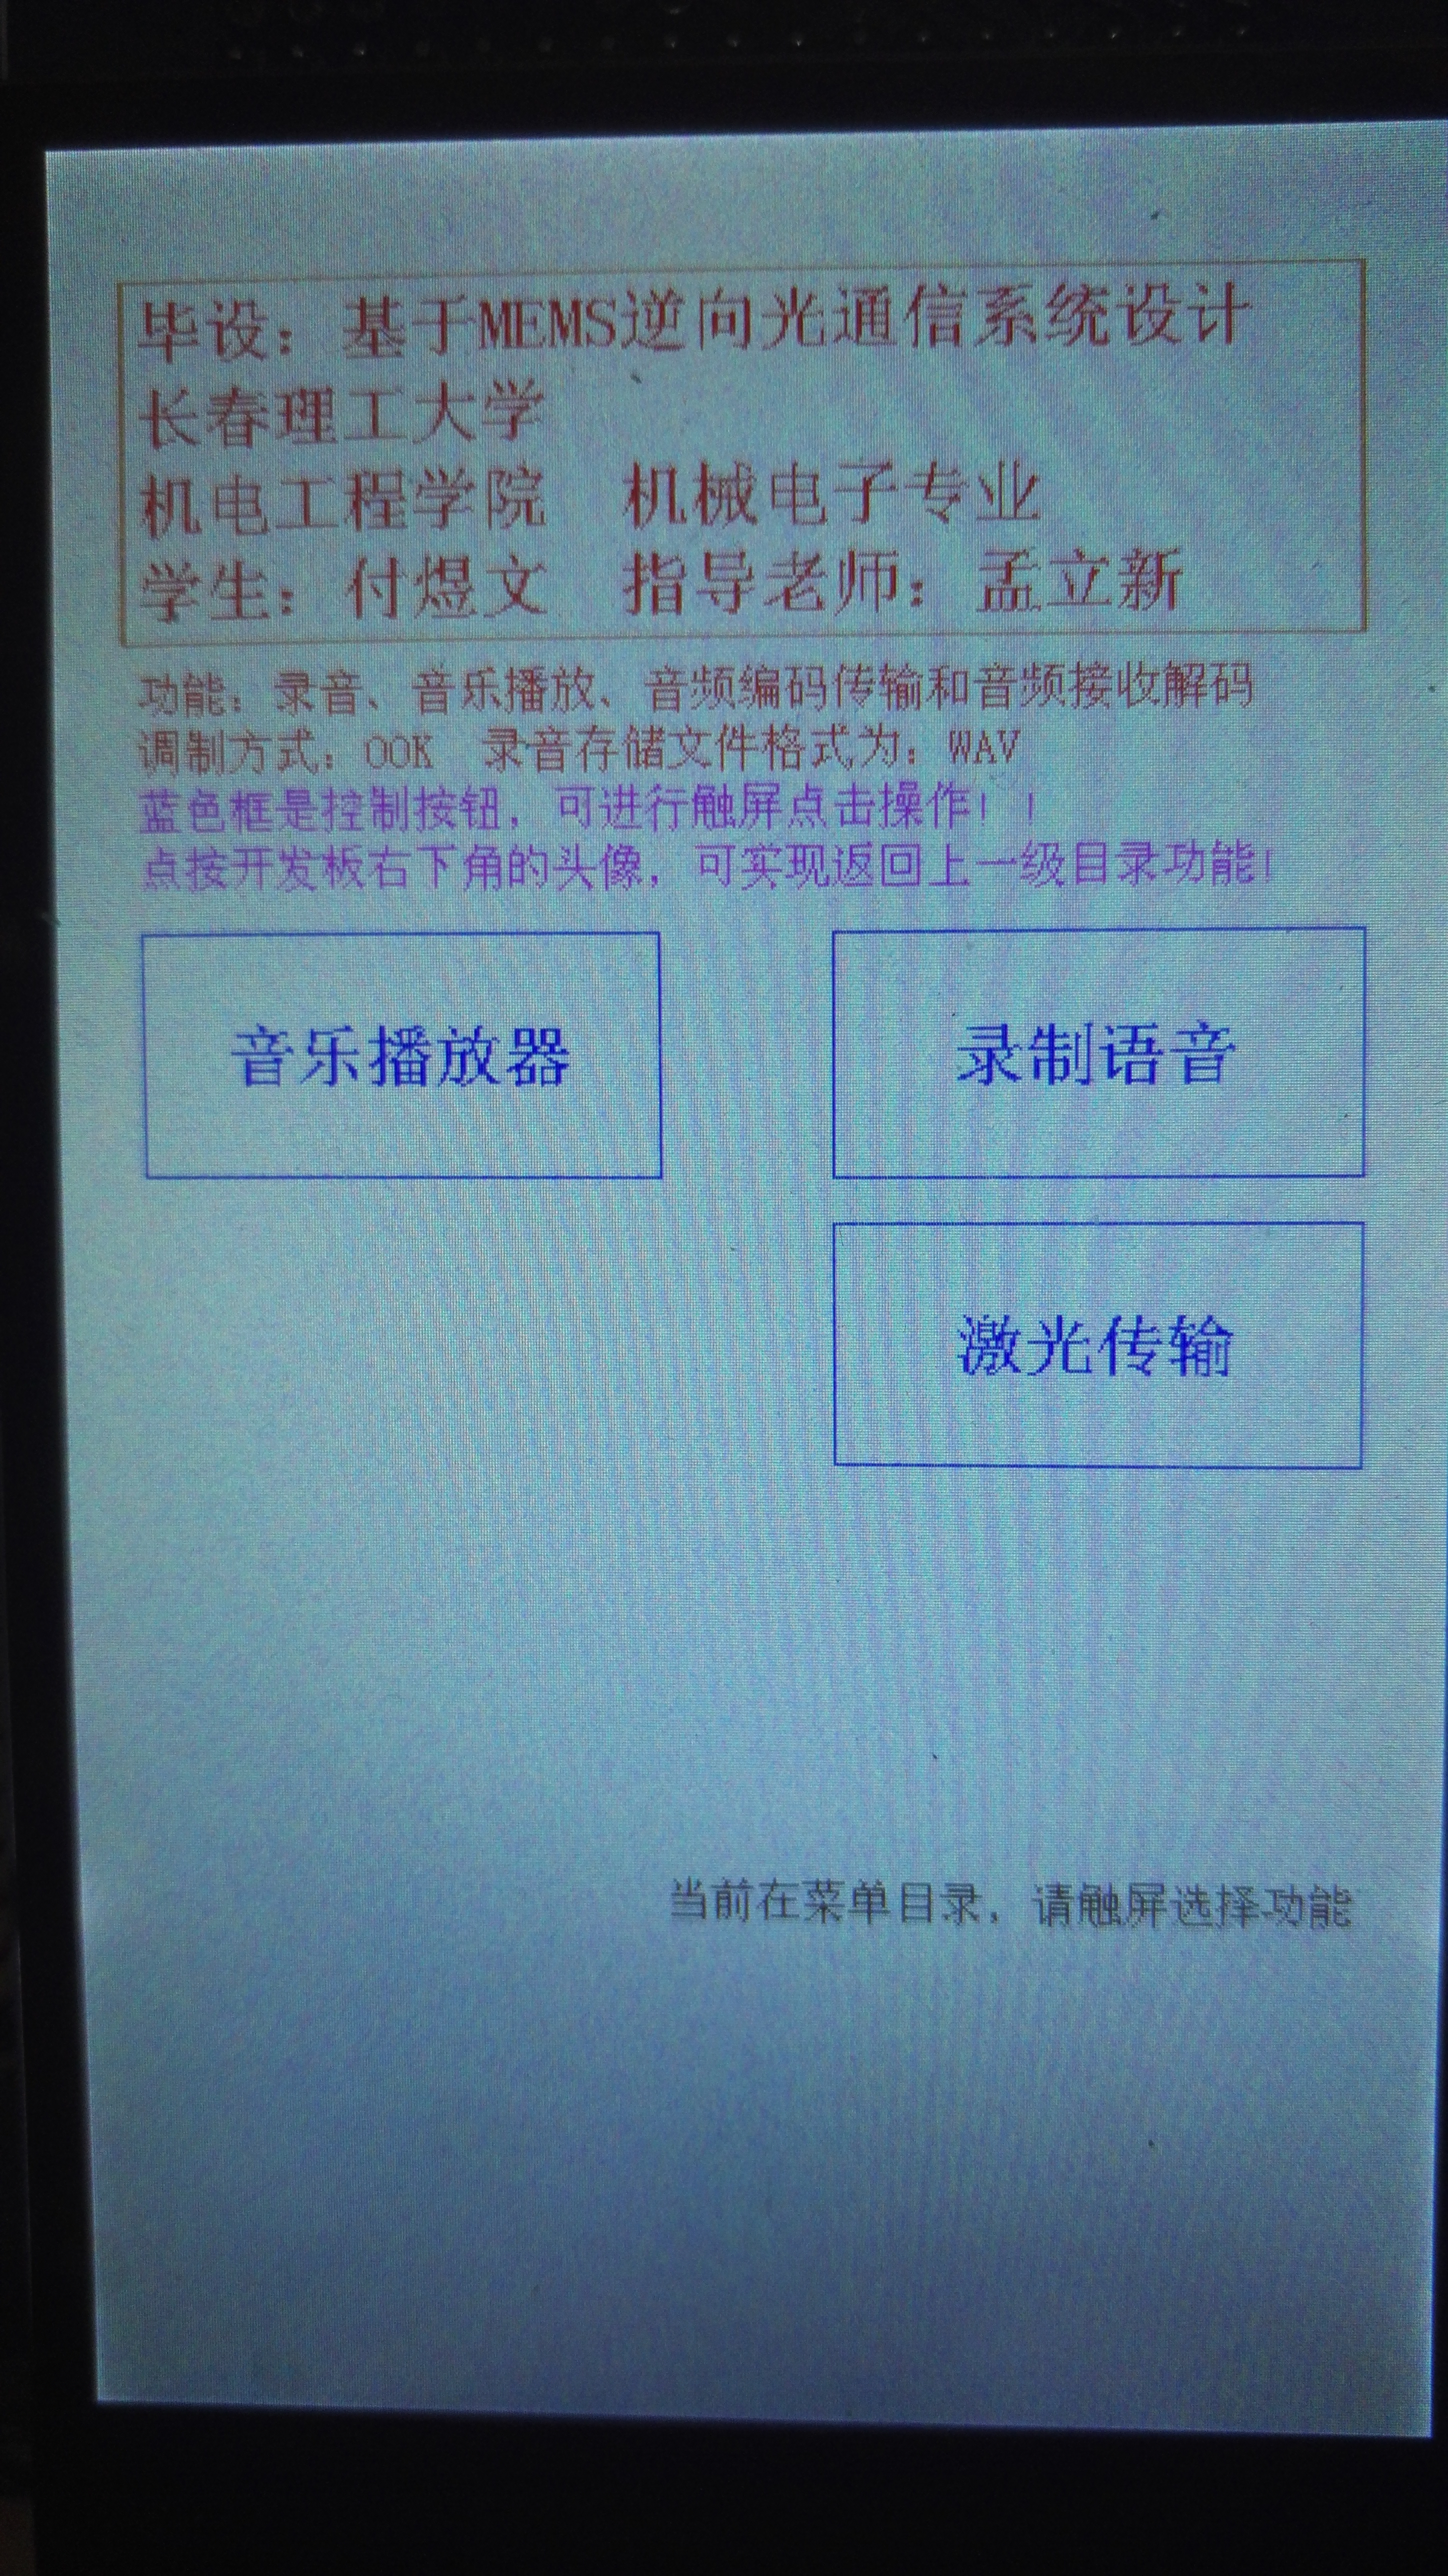
\includegraphics[width=\textwidth]{./Img/GUI-1-.jpg}
		\caption{GUI界面的一级菜单}
		\label{GUI-1-.jpg}
	\end{subfigure}%
	~
	\begin{subfigure}[c]{0.4\textwidth}
		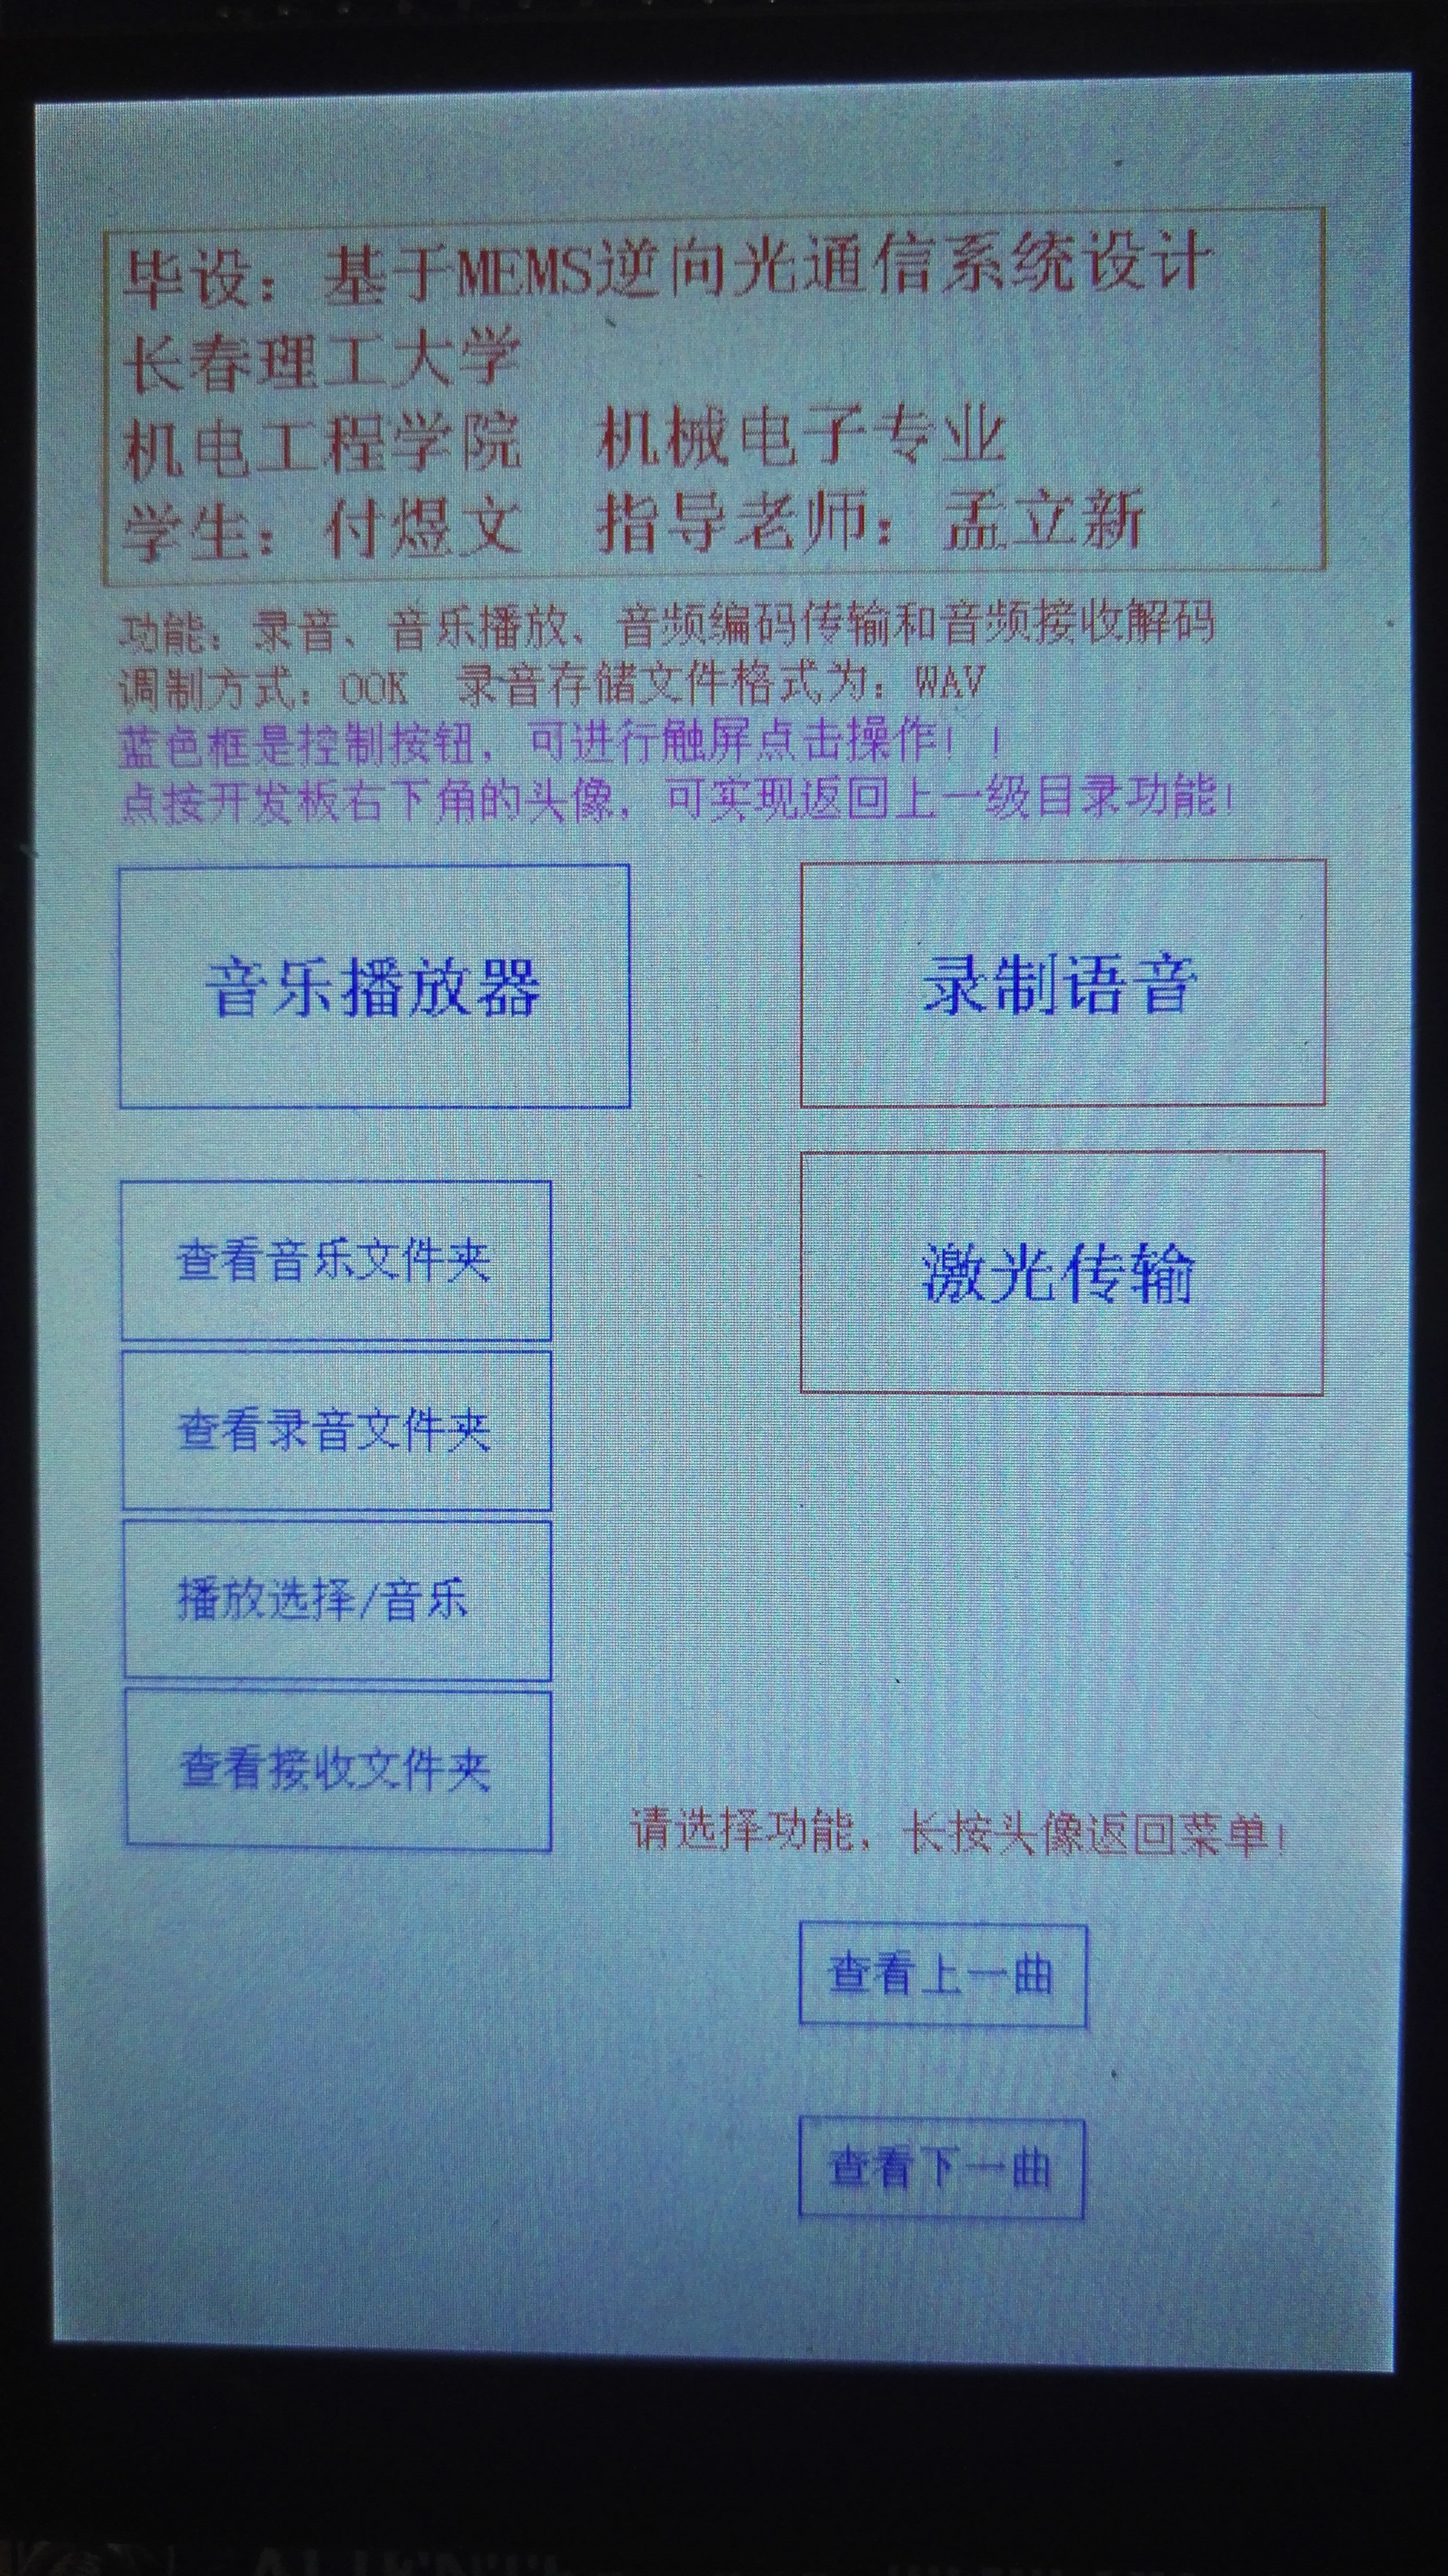
\includegraphics[width=\textwidth]{./Img/GUI-2-MSC.jpg}
		\caption{GUI界面的二级菜单:音乐播放}
		\label{GUI-2-MSC.jpg}
	\end{subfigure}%

	%add desired spacing
	\begin{subfigure}[c]{0.4\textwidth}
		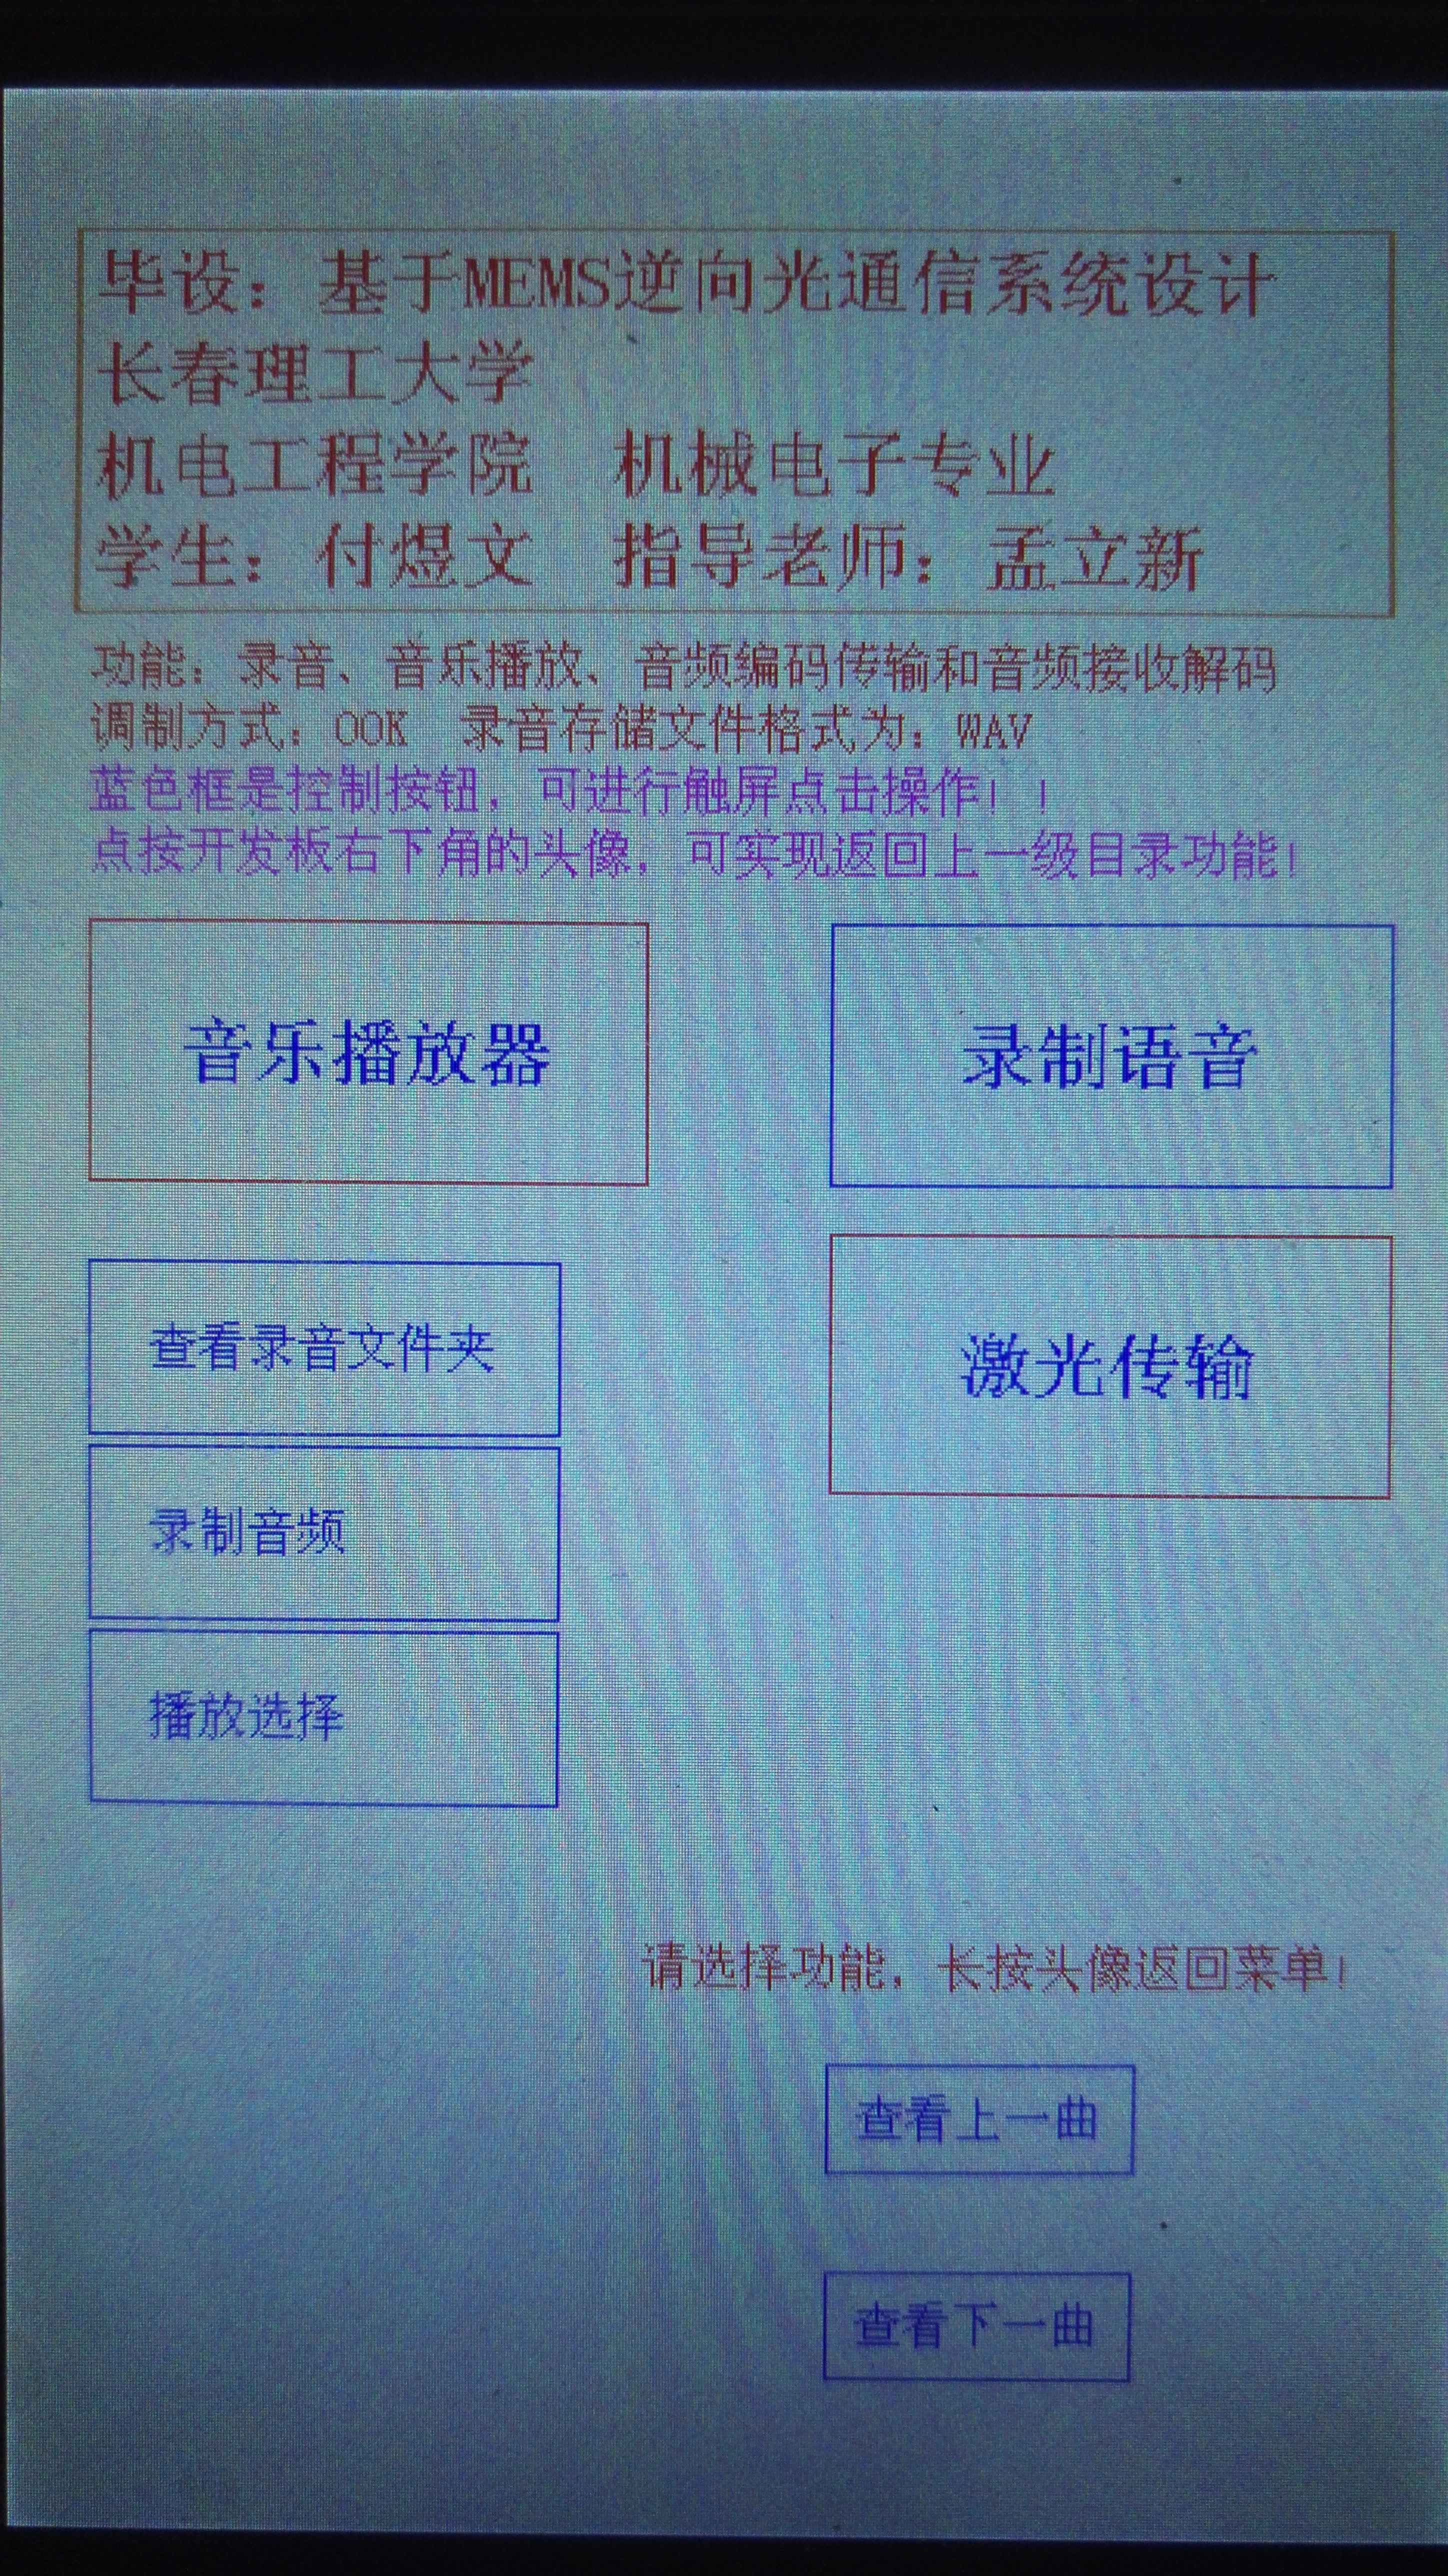
\includegraphics[width=\textwidth]{./Img/GUI-2-REC.jpg}
		\caption{二级菜单:录制音频}
		\label{GUI-2-REC.jpg}
	\end{subfigure}
	~
	\begin{subfigure}[c]{0.4\textwidth}
	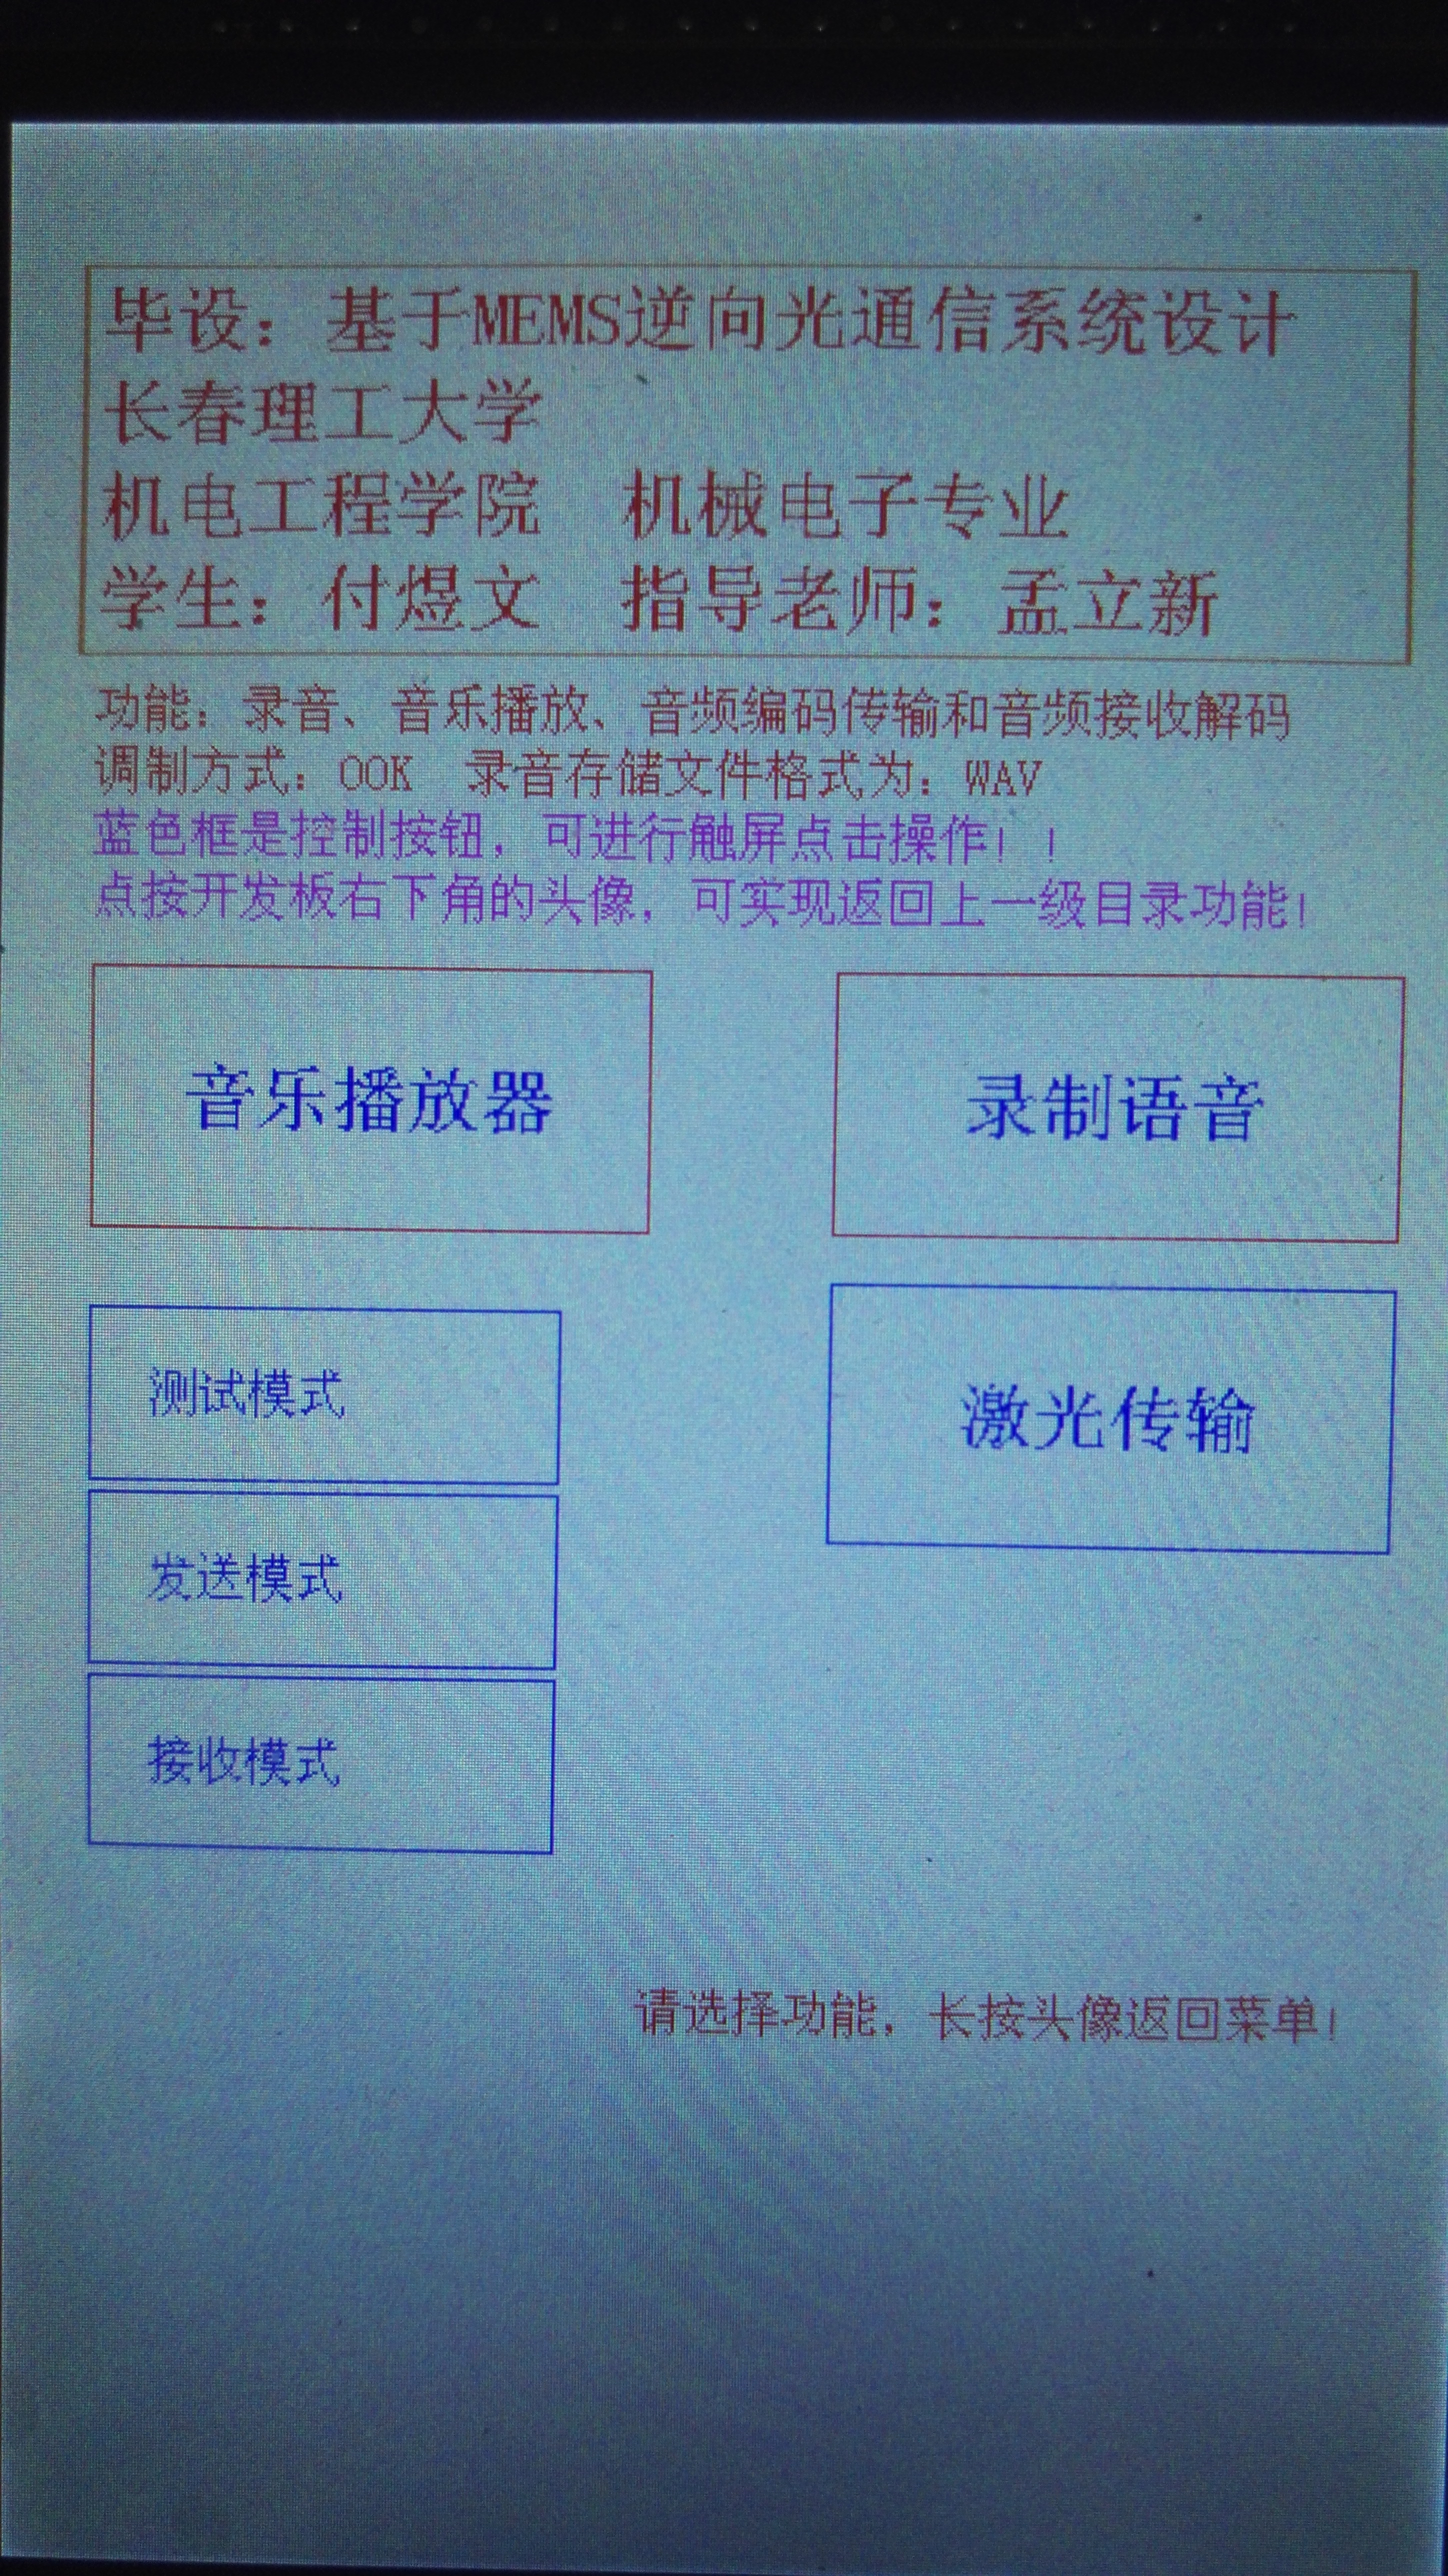
\includegraphics[width=\textwidth]{./Img/GUI-2-TRANS.jpg}
	\caption{GUI界面的二级菜单:激光传输}
	\label{GUI-2-TRANS.jpg}
	\end{subfigure}
	\caption{STM32单片机GUI界面设计}
	%\bicaption{STM32单片机GUI界面设计\ (a) GUI界面的一级菜单,(b)GUI界面的二级菜单:音乐播放 ,(c)二级菜单:录制音频,(d)GUI界面的二级菜单:激光传输。}{GUI DESIGN.(a)GUI MAIN ,(b) GUI SECOND MUSIC, (c)GUI SECOND RECORDING ,(d)GUI SECOND LASER.}
\end{figure}


图~\ref{GUI-2-MSC-1.jpg}中展示的是GUI界面的二级菜单:音乐播放——查看音乐文件夹。


图~\ref{GUI-2-MSC-2.jpg}中展示的是GUI界面的二级菜单:音乐播放——查看录音文件夹。


图~\ref{GUI-2-MSC-3.jpg}中展示的是GUI界面的二级菜单:音乐播放——播放当前选择。

图~\ref{GUI-2-MSC-5.jpg}中展示的是GUI界面的二级菜单:音乐播放——查看接收文件夹。

\begin{figure}[!htbp]
	\centering
	\begin{subfigure}[c]{0.4\textwidth}
		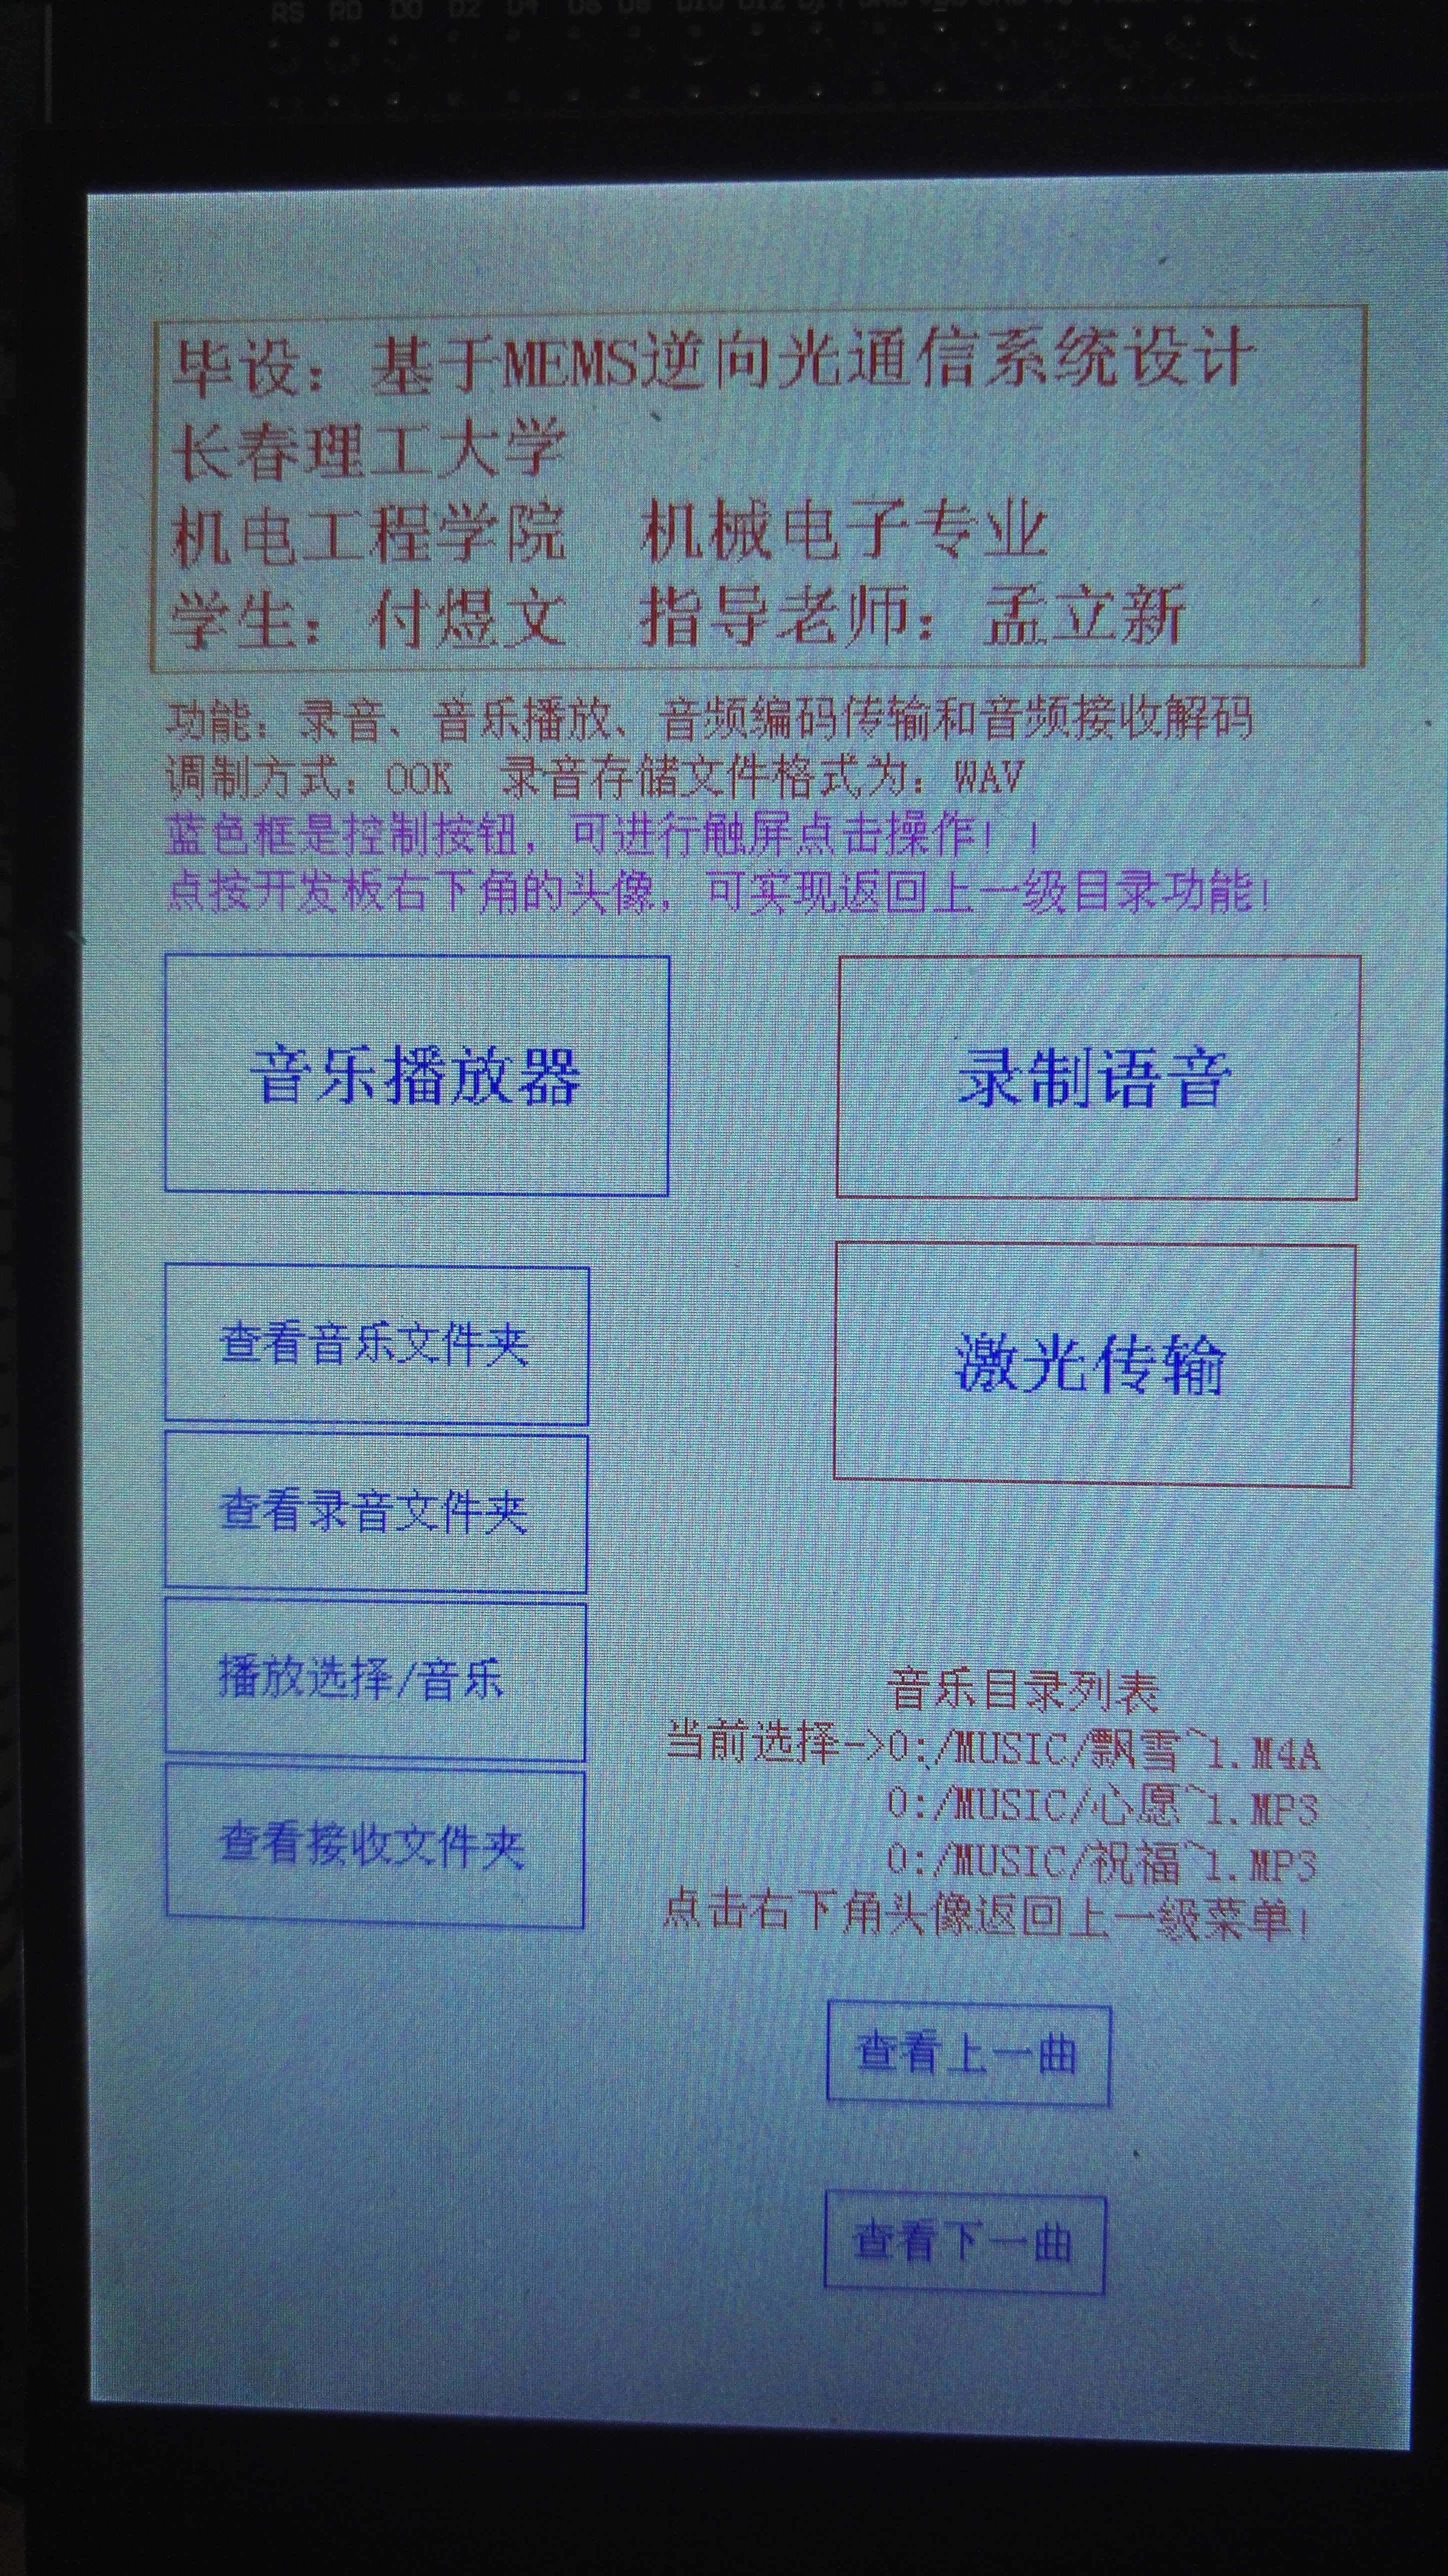
\includegraphics[width=\textwidth]{./Img/GUI-2-MSC-1.jpg}
		\caption{查看音乐文件夹}
		\label{GUI-2-MSC-1.jpg}
	\end{subfigure}%
	~
	\begin{subfigure}[c]{0.4\textwidth}
		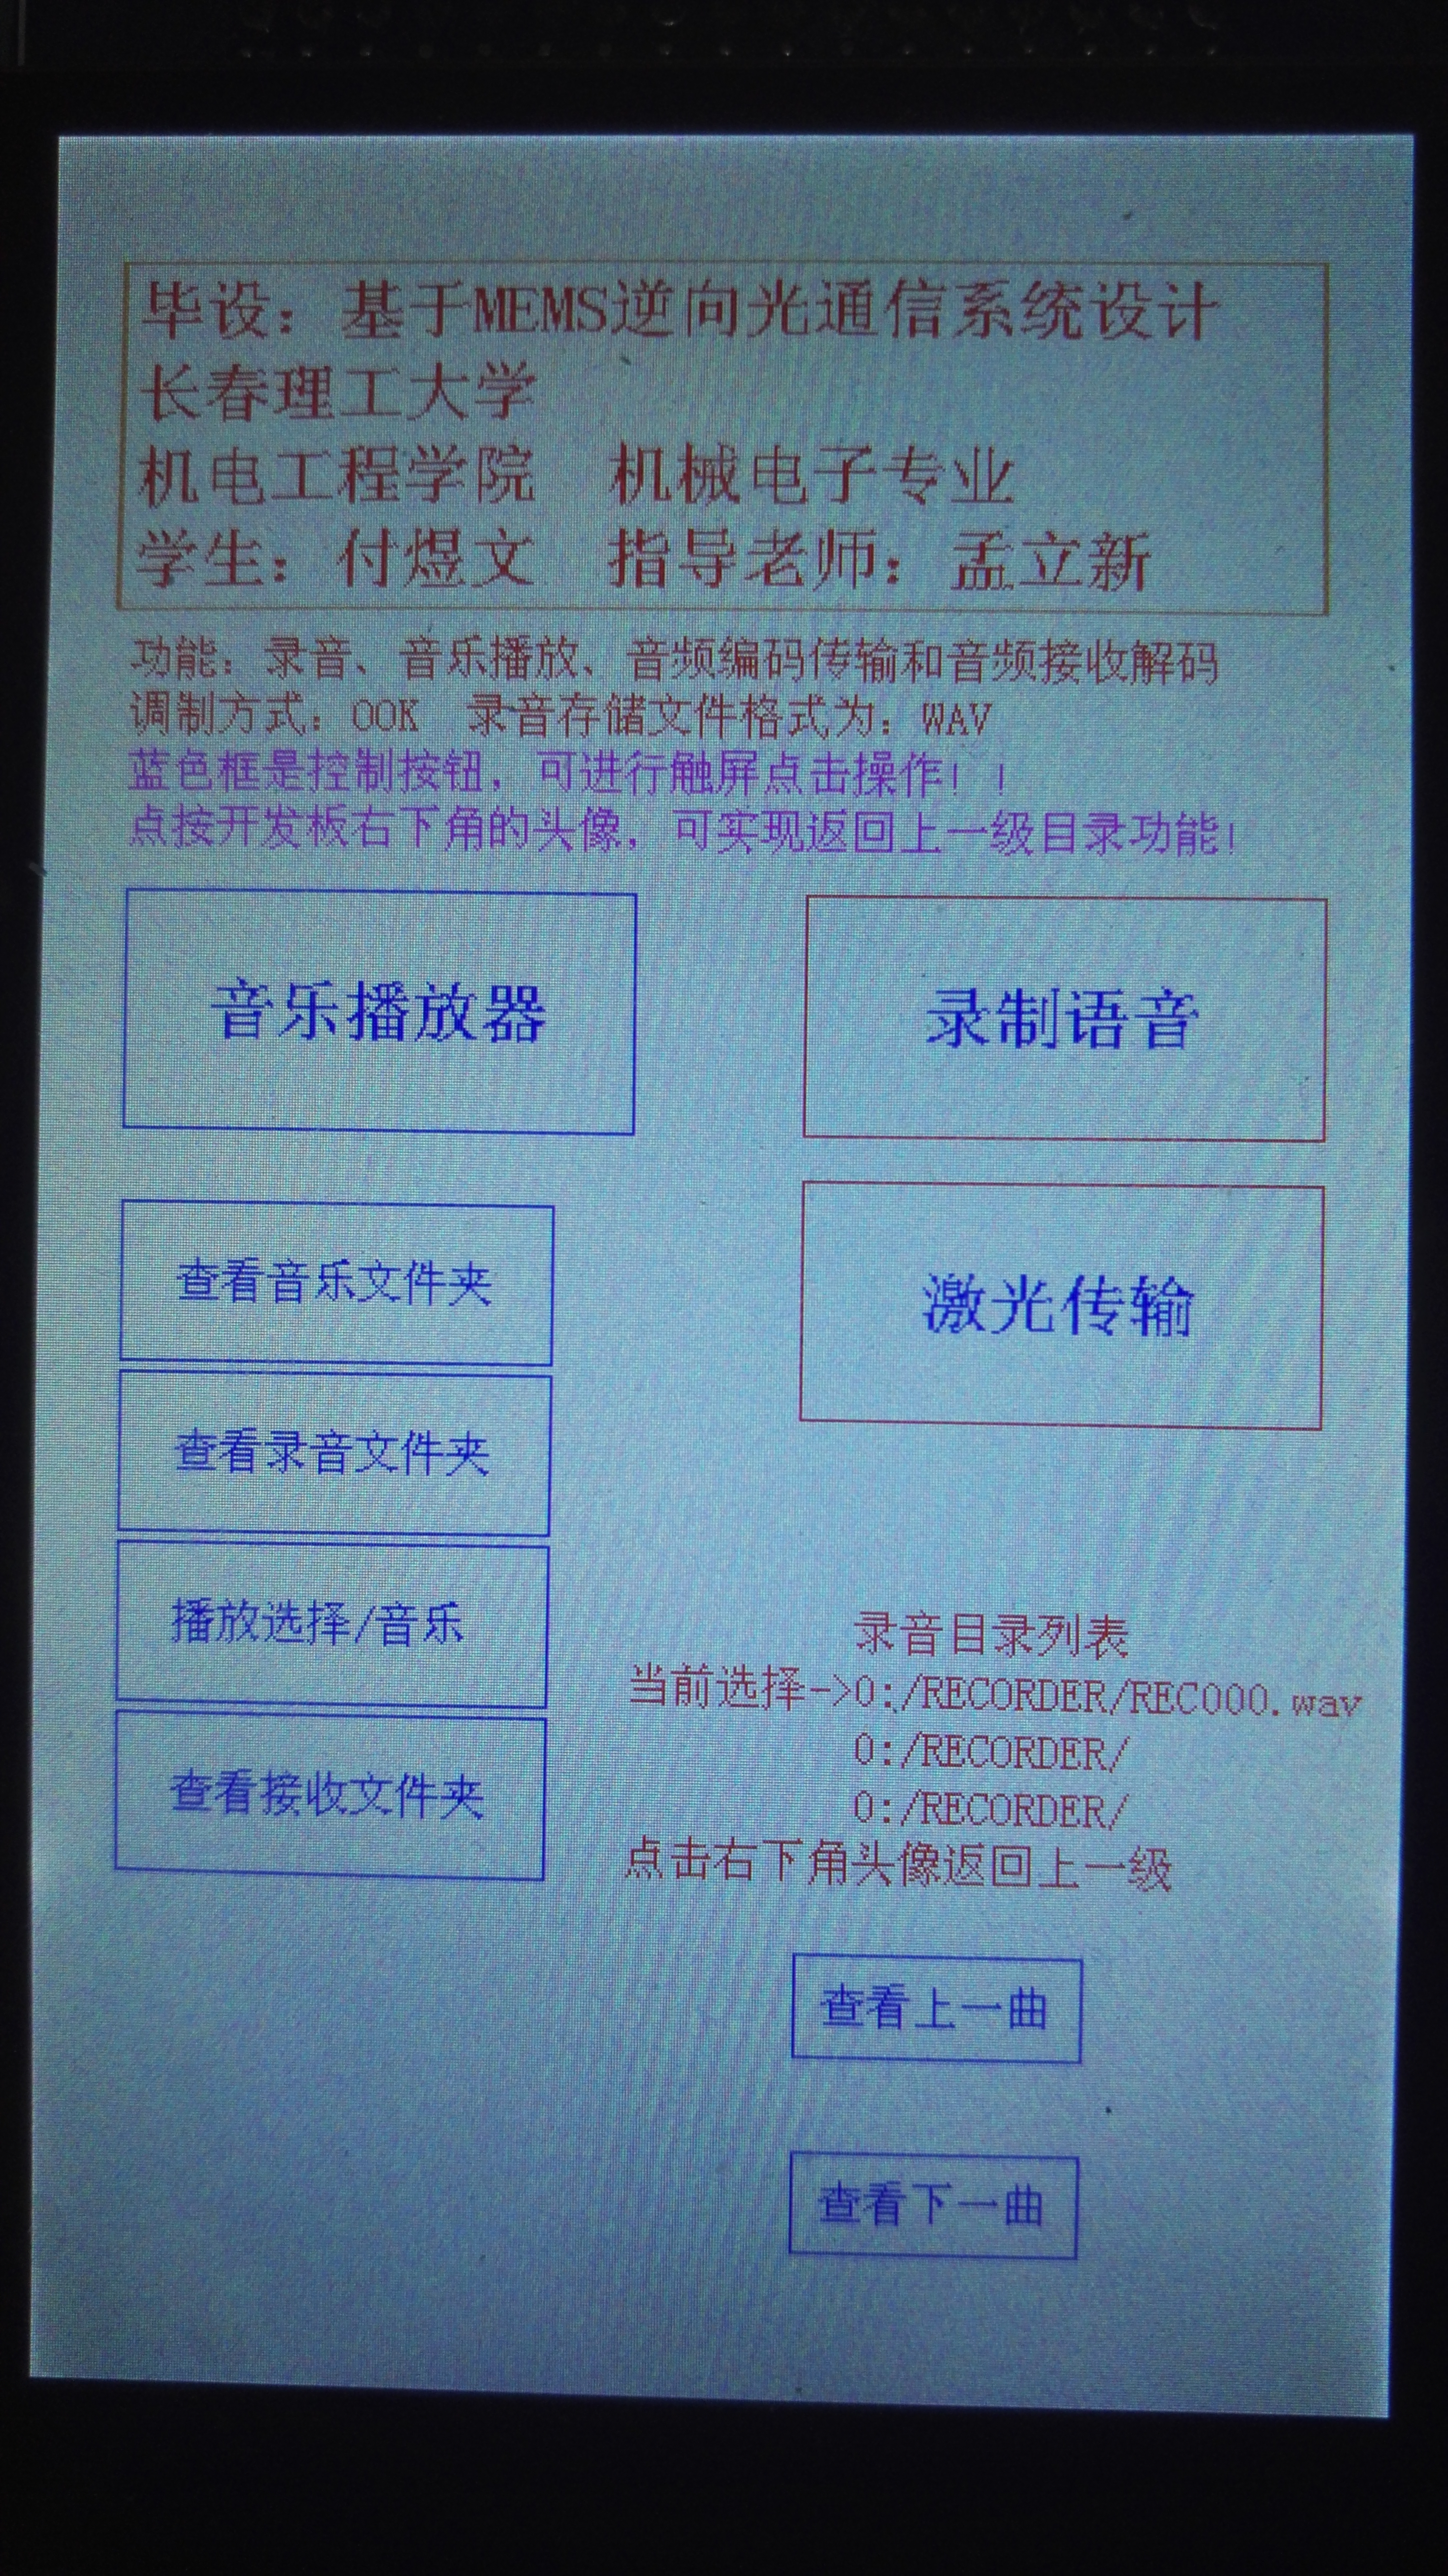
\includegraphics[width=\textwidth]{./Img/GUI-2-MSC-2.jpg}
		\caption{查看录音文件夹}
		\label{GUI-2-MSC-2.jpg}
	\end{subfigure}%
	
	%add desired spacing
	\begin{subfigure}[c]{0.4\textwidth}
		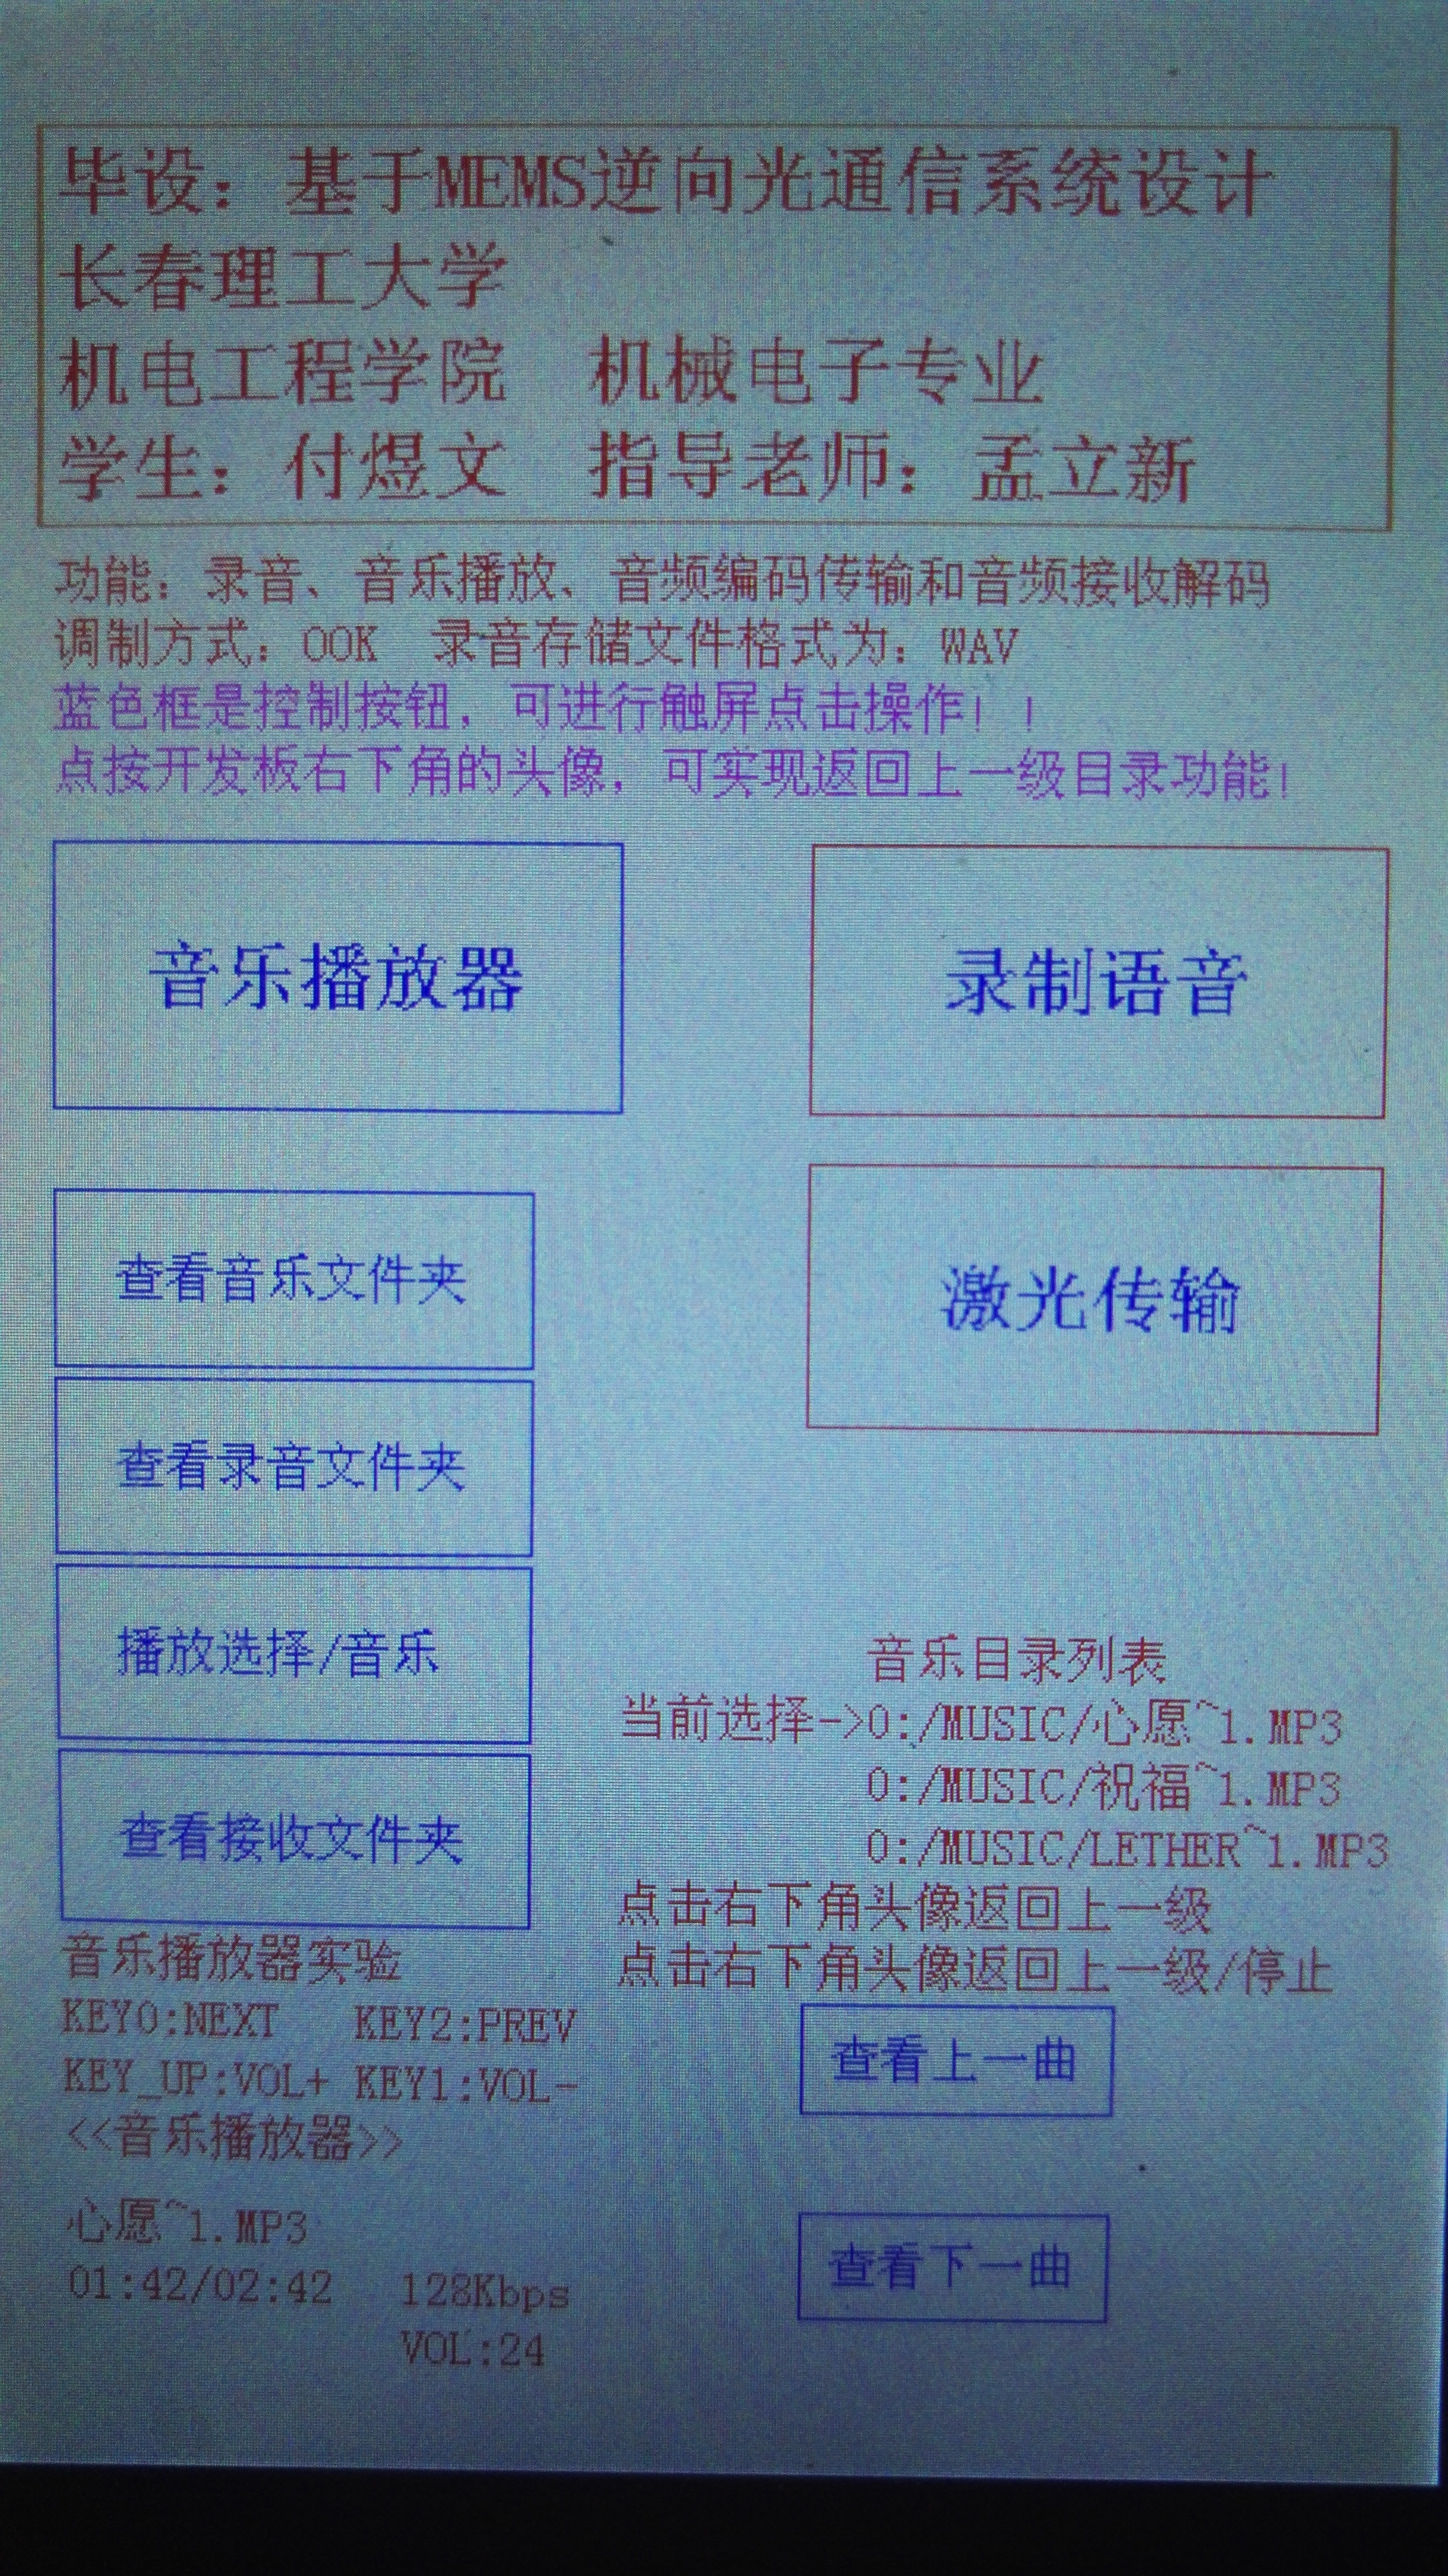
\includegraphics[width=\textwidth]{./Img/GUI-2-MSC-3.jpg}
		\caption{播放当前选择}
		\label{GUI-2-MSC-3.jpg}
	\end{subfigure}
	~
	\begin{subfigure}[c]{0.4\textwidth}
		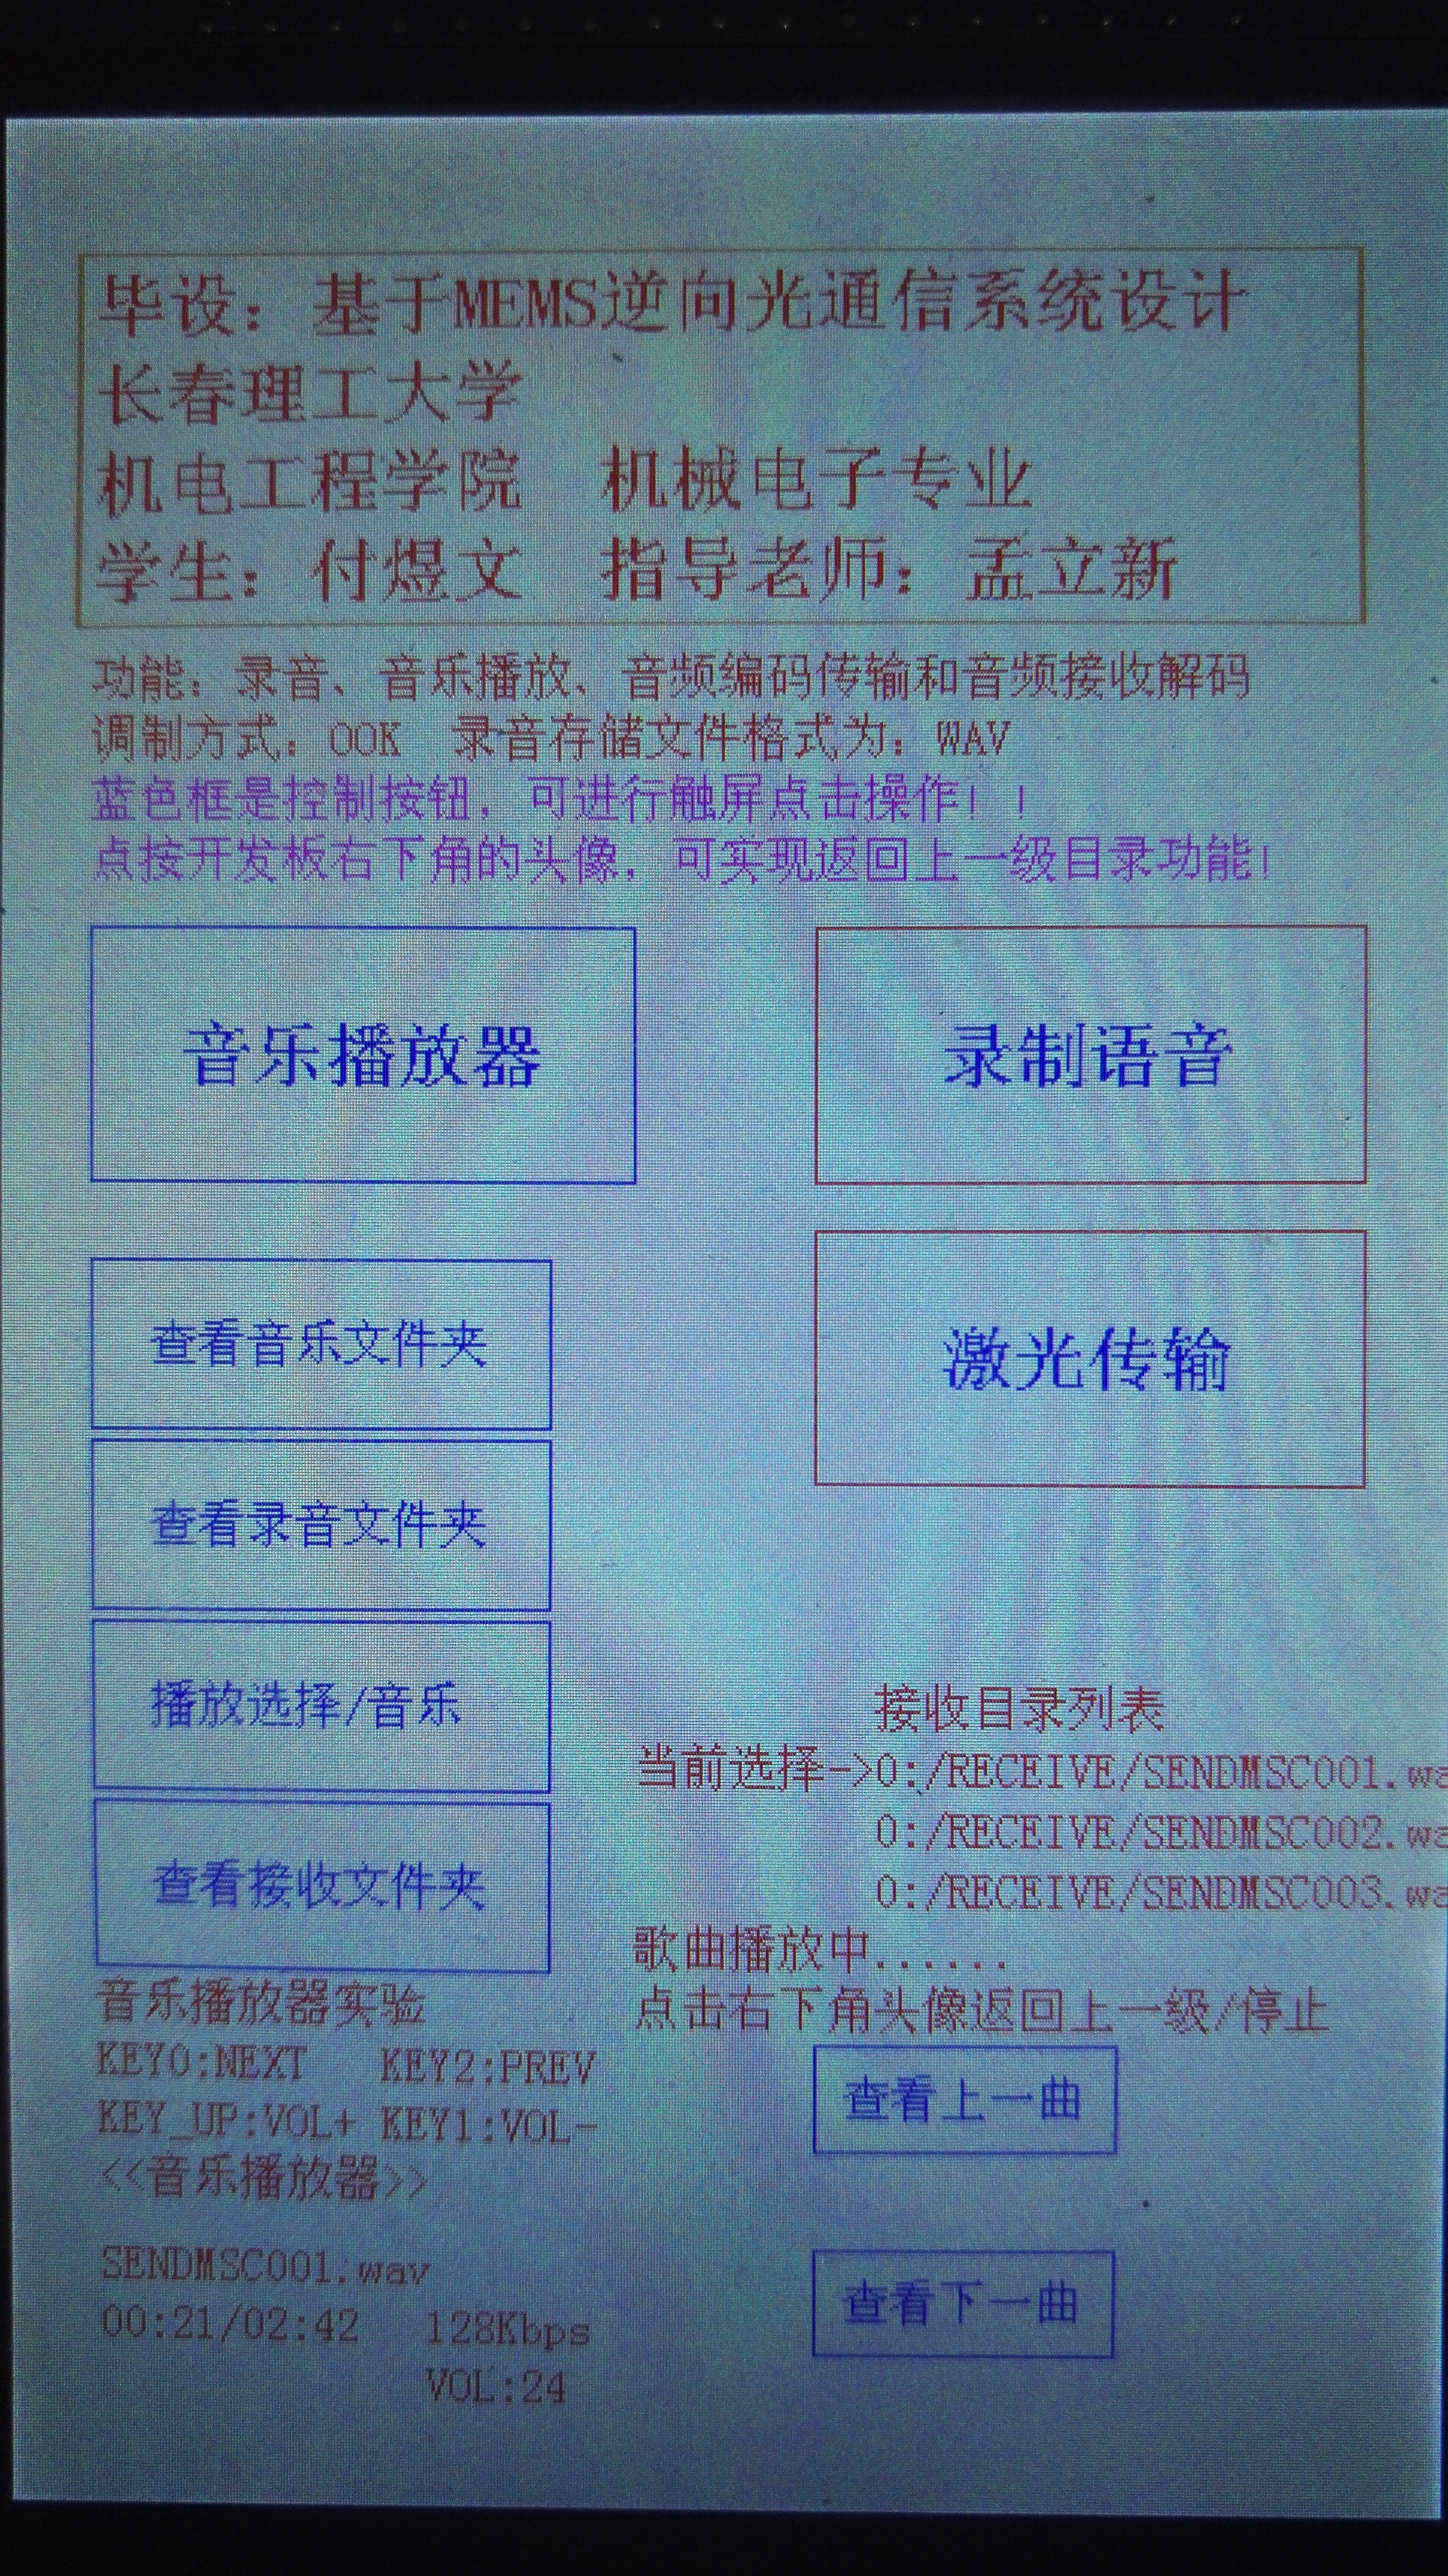
\includegraphics[width=\textwidth]{./Img/GUI-2-MSC-5.jpg}
		\caption{查看接收文件夹}
		\label{GUI-2-MSC-5.jpg}
	\end{subfigure}
	\caption{GUI界面的二级菜单:音乐播放}
	%\bicaption{GUI界面的二级菜单:音乐播放。(a)查看音乐文件夹,(b)查看录音文件夹 ,(c)播放当前选择,(d)查看接收文件夹。}{GUI DESIGN.}
\end{figure}

图~\ref{GUI-2-REC-1.jpg}中展示的是GUI界面的二级菜单:录制语音——查看录音文件夹。


图~\ref{GUI-2-REC-2.jpg}中展示的是GUI界面的二级菜单:录制语音——录制音频。


图~\ref{GUI-2-REC-3.jpg}中展示的是GUI界面的二级菜单:录制语音——播放选择。

\begin{figure}[!htbp]
	\centering
	\begin{subfigure}[c]{0.4\textwidth}
		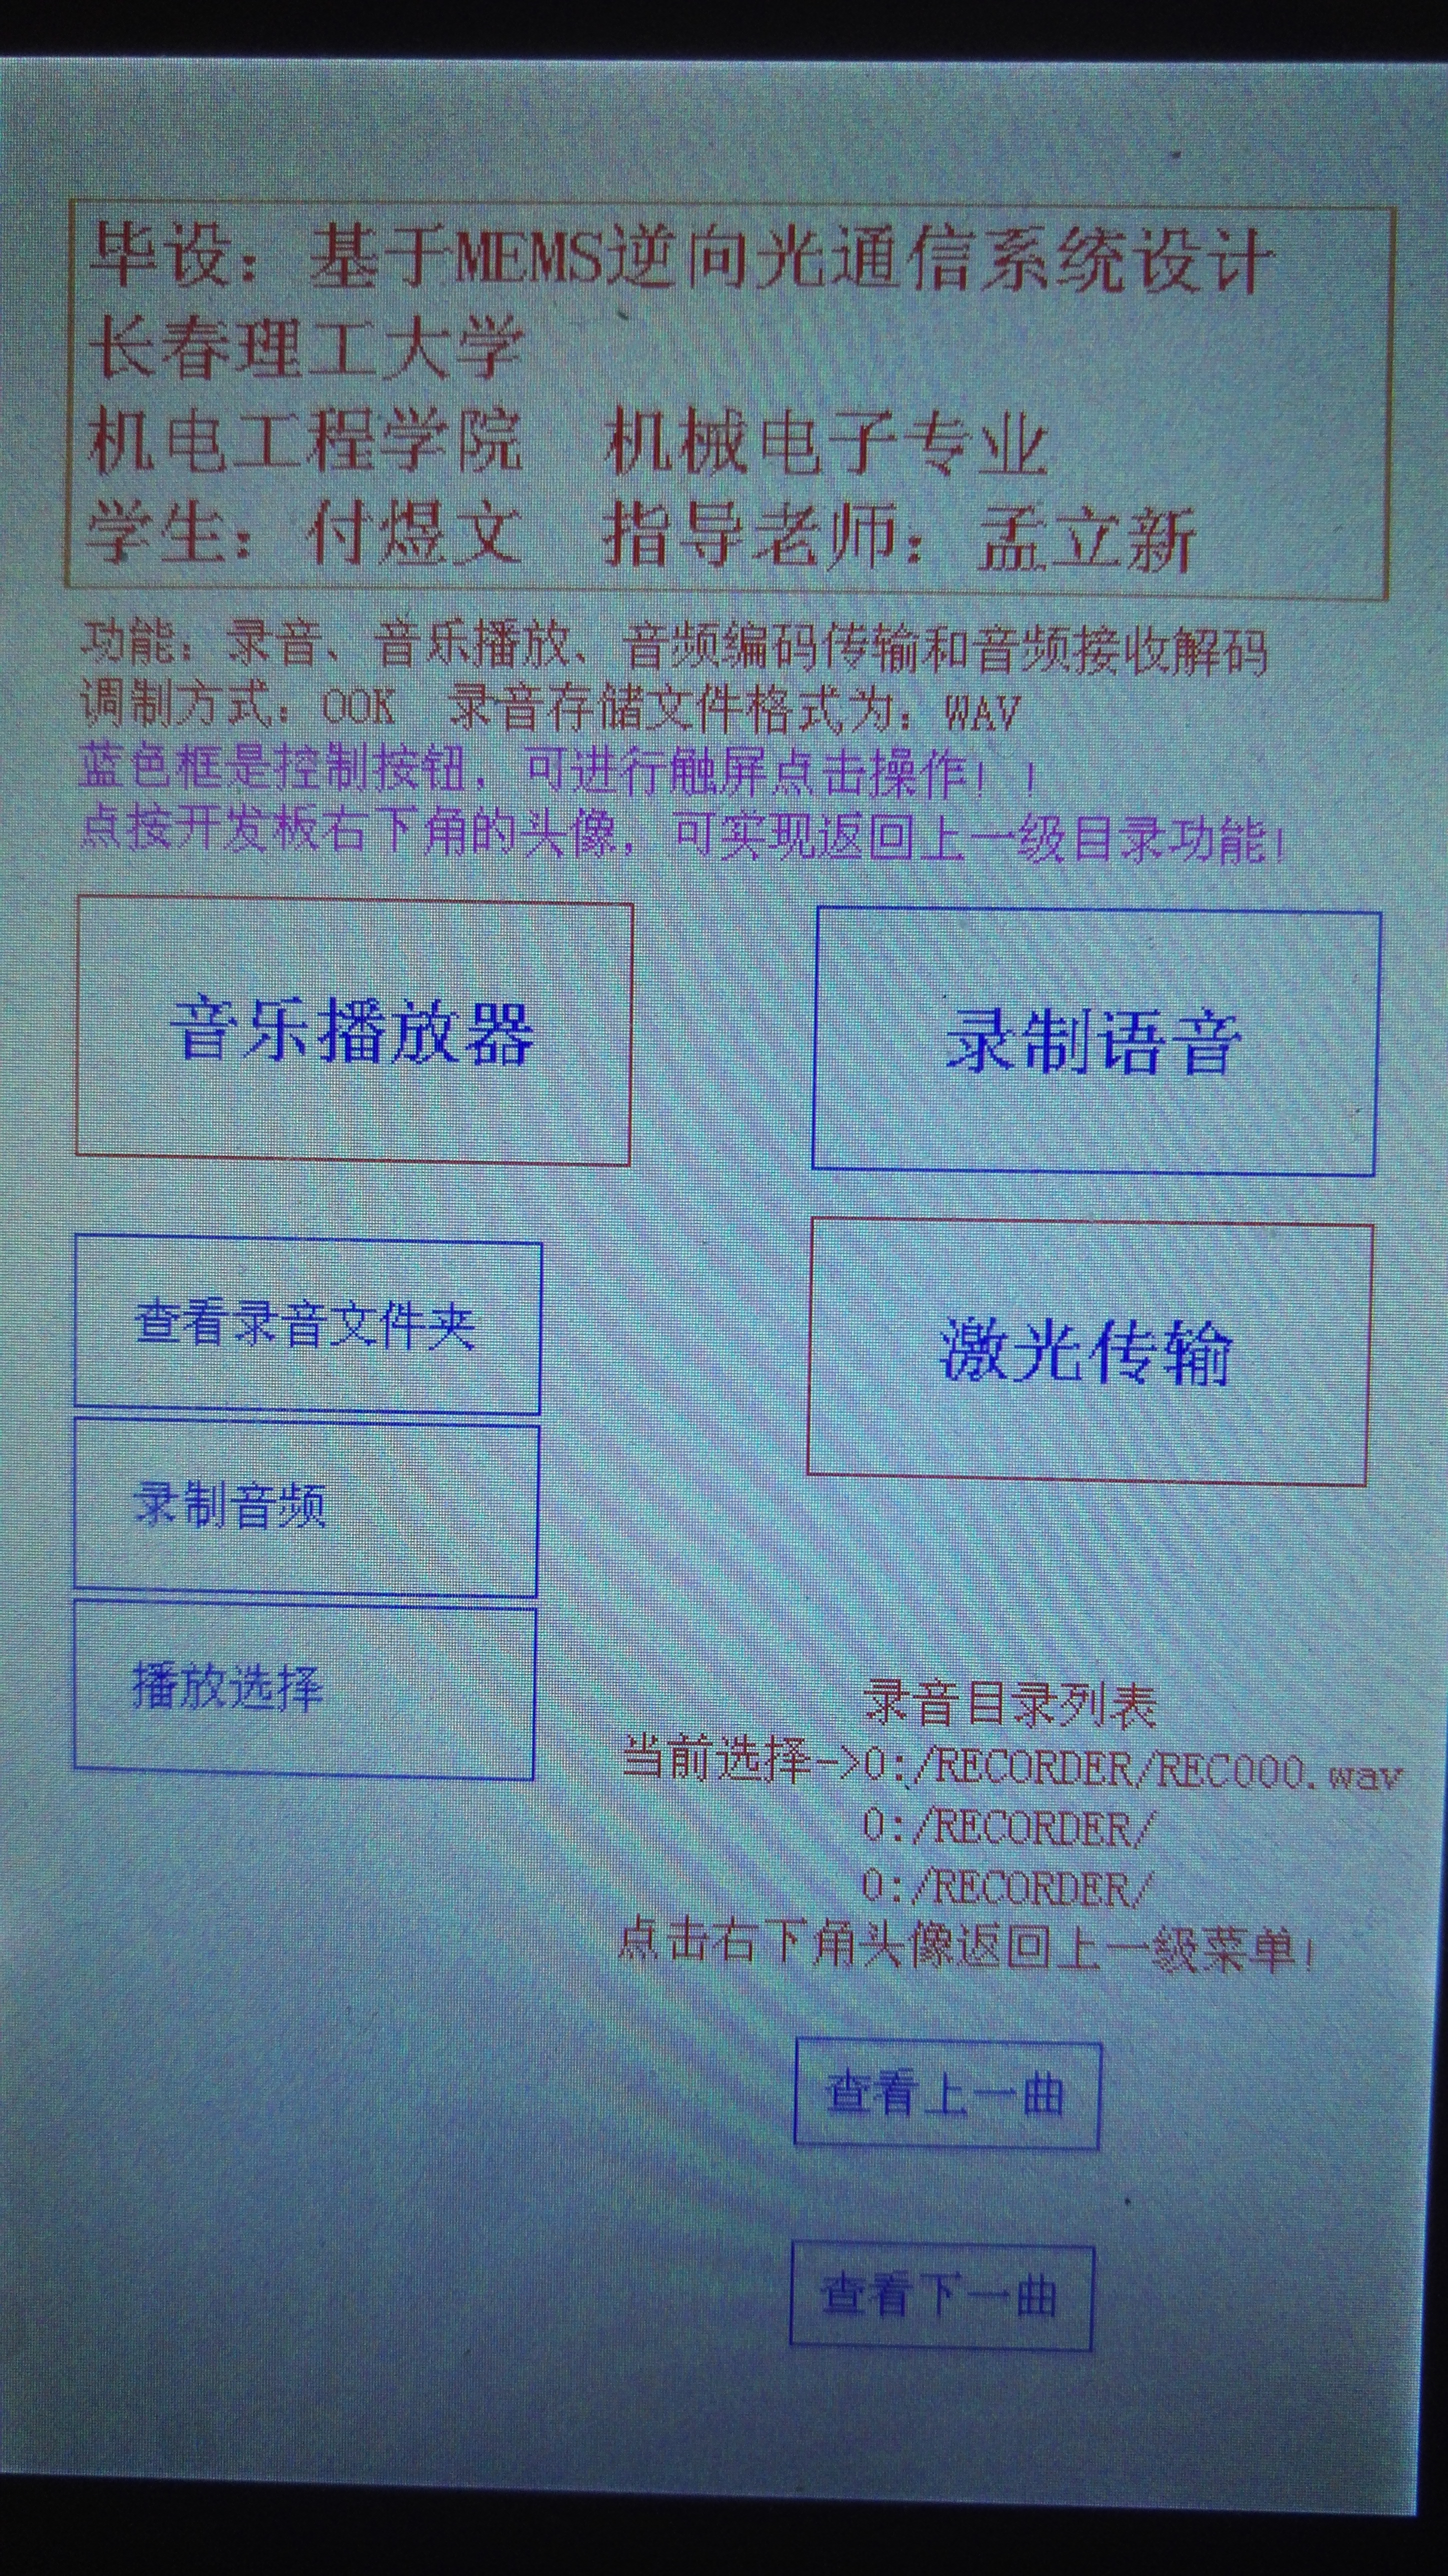
\includegraphics[width=\textwidth]{./Img/GUI-2-REC-1.jpg}
		\caption{查看录音文件夹}
		\label{GUI-2-REC-1.jpg}
	\end{subfigure}%
	~
	\begin{subfigure}[c]{0.4\textwidth}
		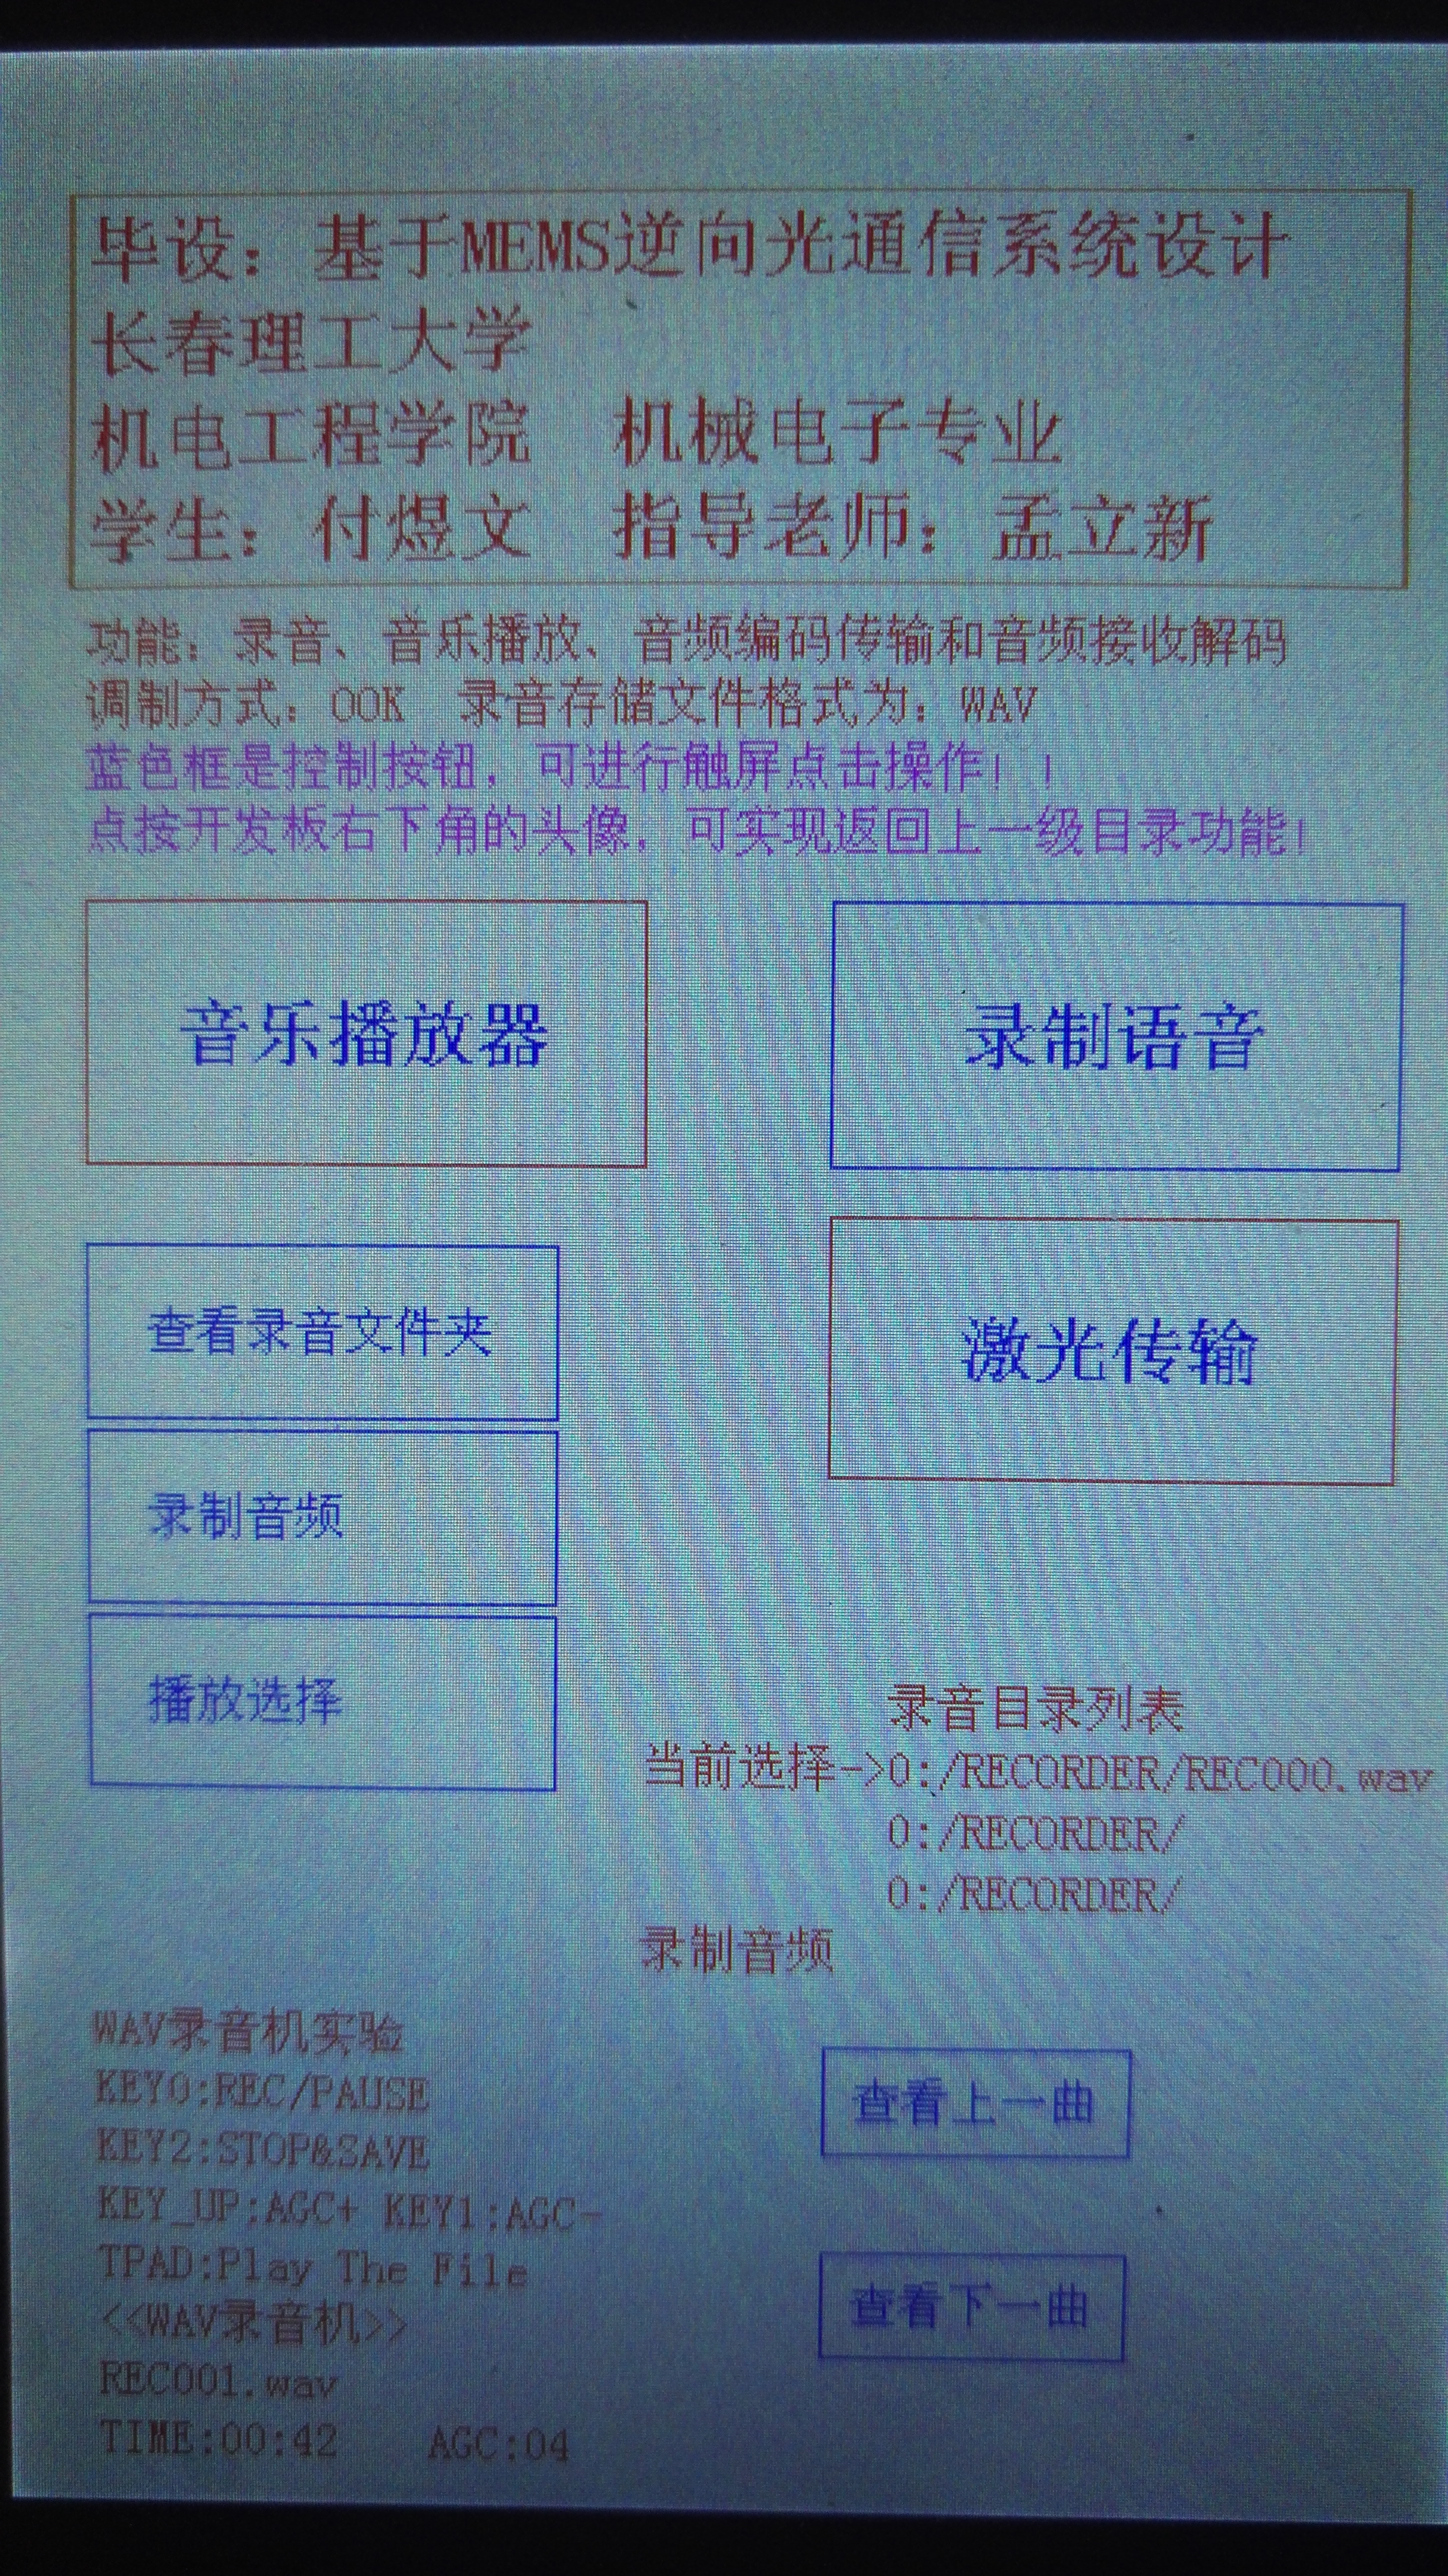
\includegraphics[width=\textwidth]{./Img/GUI-2-REC-2.jpg}
		\caption{录制音频}
		\label{GUI-2-REC-2.jpg}
	\end{subfigure}%

	%add desired spacing
	\begin{subfigure}[c]{0.4\textwidth}
		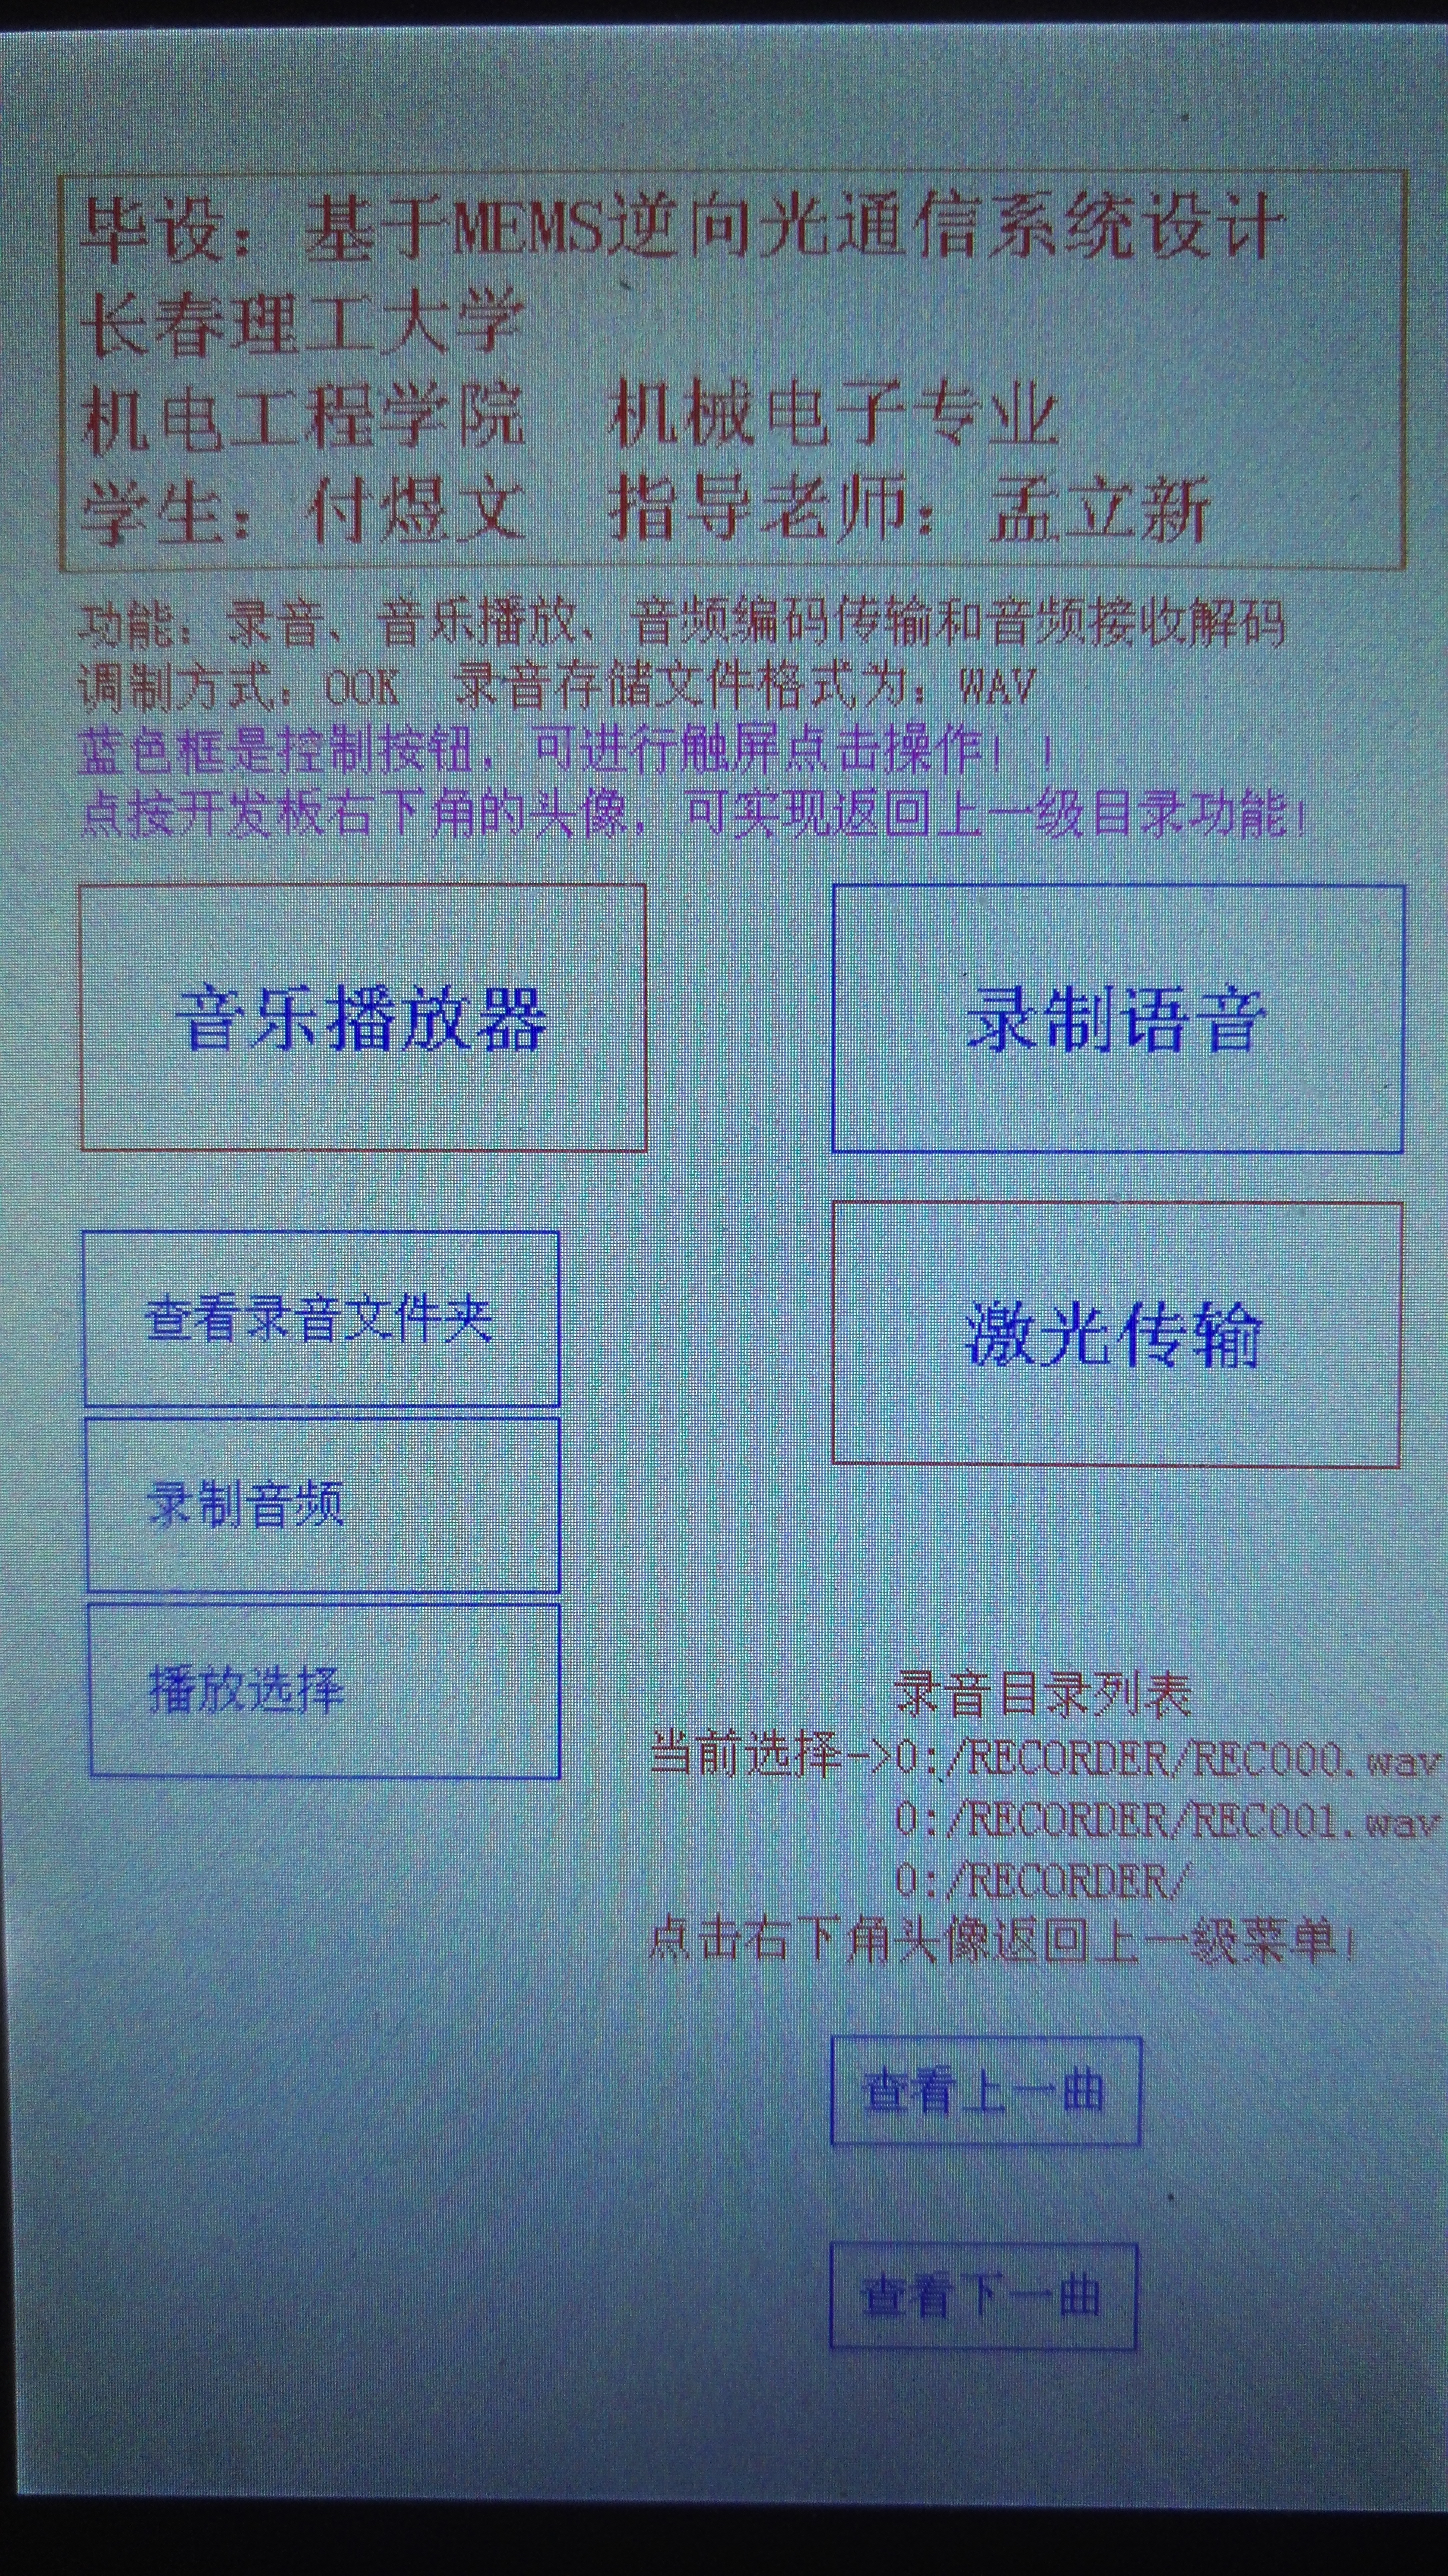
\includegraphics[width=\textwidth]{./Img/GUI-2-REC-3.jpg}
		\caption{播放当前选择}
		\label{GUI-2-REC-3.jpg}
	\end{subfigure}
	\caption{GUI界面的二级菜单:录制音频}
	%\bicaption{GUI界面的二级菜单:录制音频。(a)查看录音文件夹,(b)录制音频 ,(c)播放当前选择。}{GUI SECOND RECORDING.}
\end{figure}

\begin{figure}[!htbp]
	\centering
	\begin{subfigure}[c]{0.4\textwidth}
		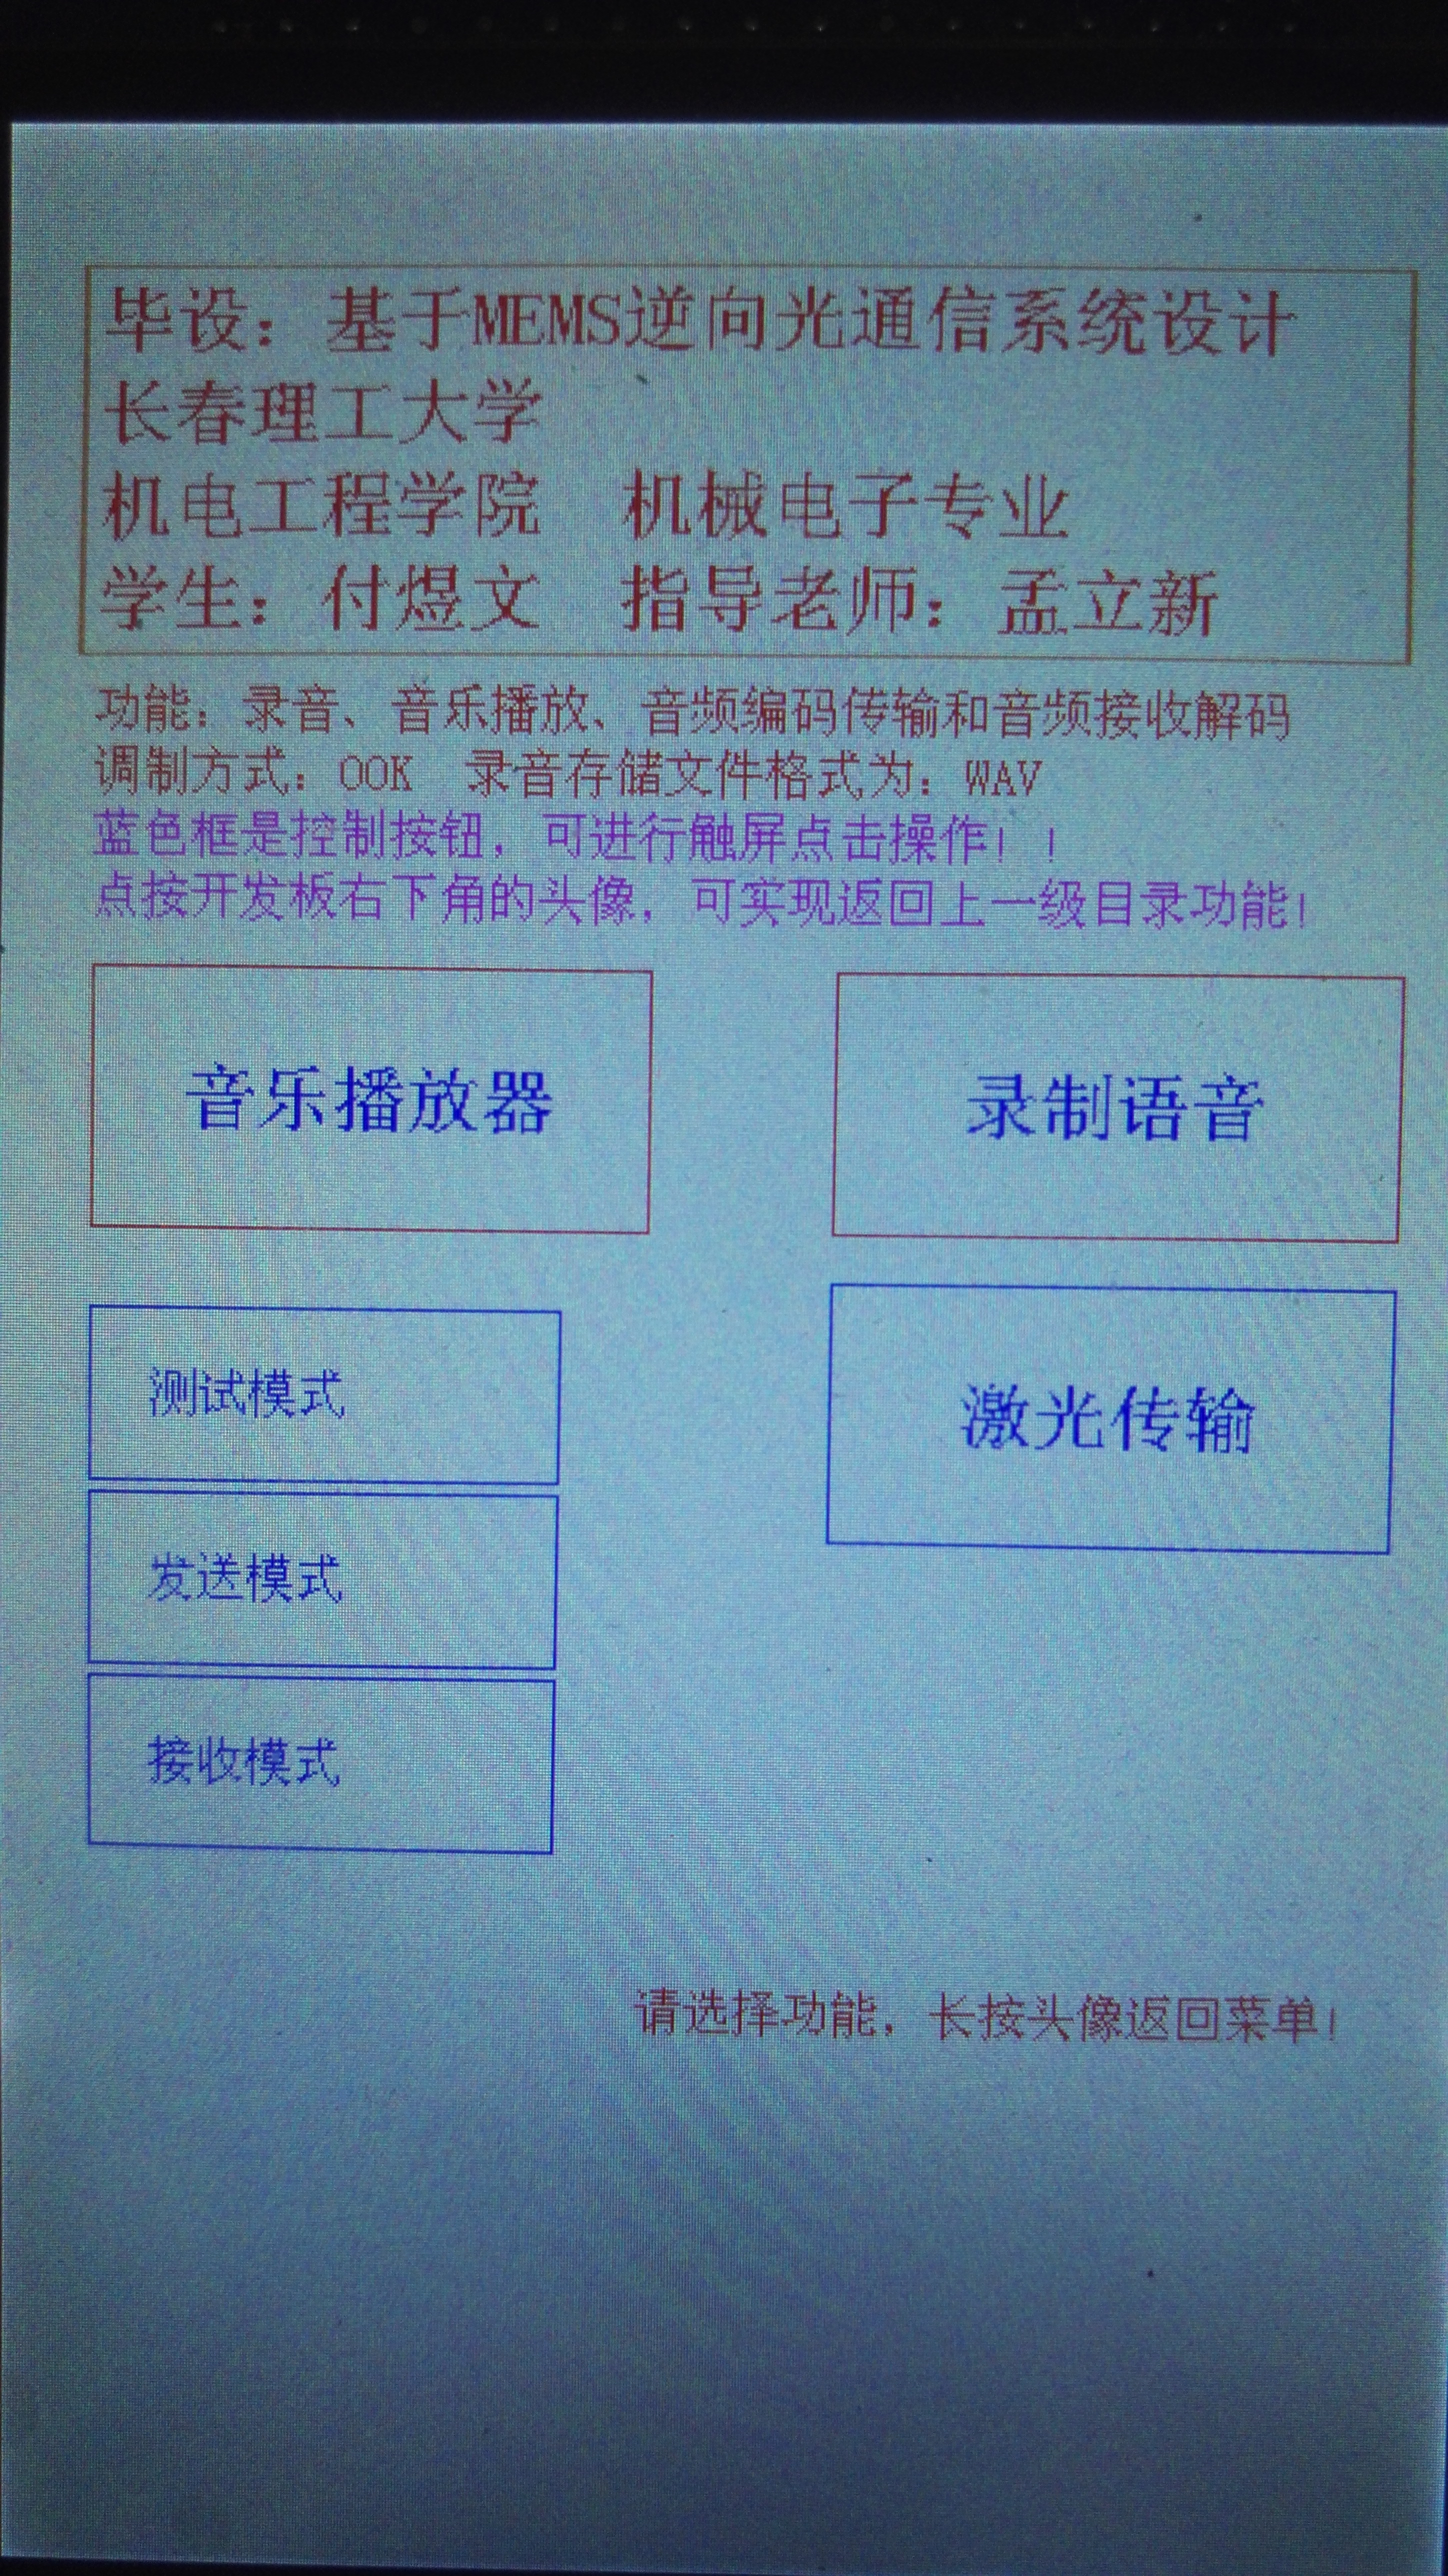
\includegraphics[width=\textwidth]{./Img/GUI-2-TRANS.jpg}
		\caption{激光传输主菜单}
		\label{GUI-2-TRANS1.jpg}
	\end{subfigure}
~	
	\begin{subfigure}[c]{0.4\textwidth}
		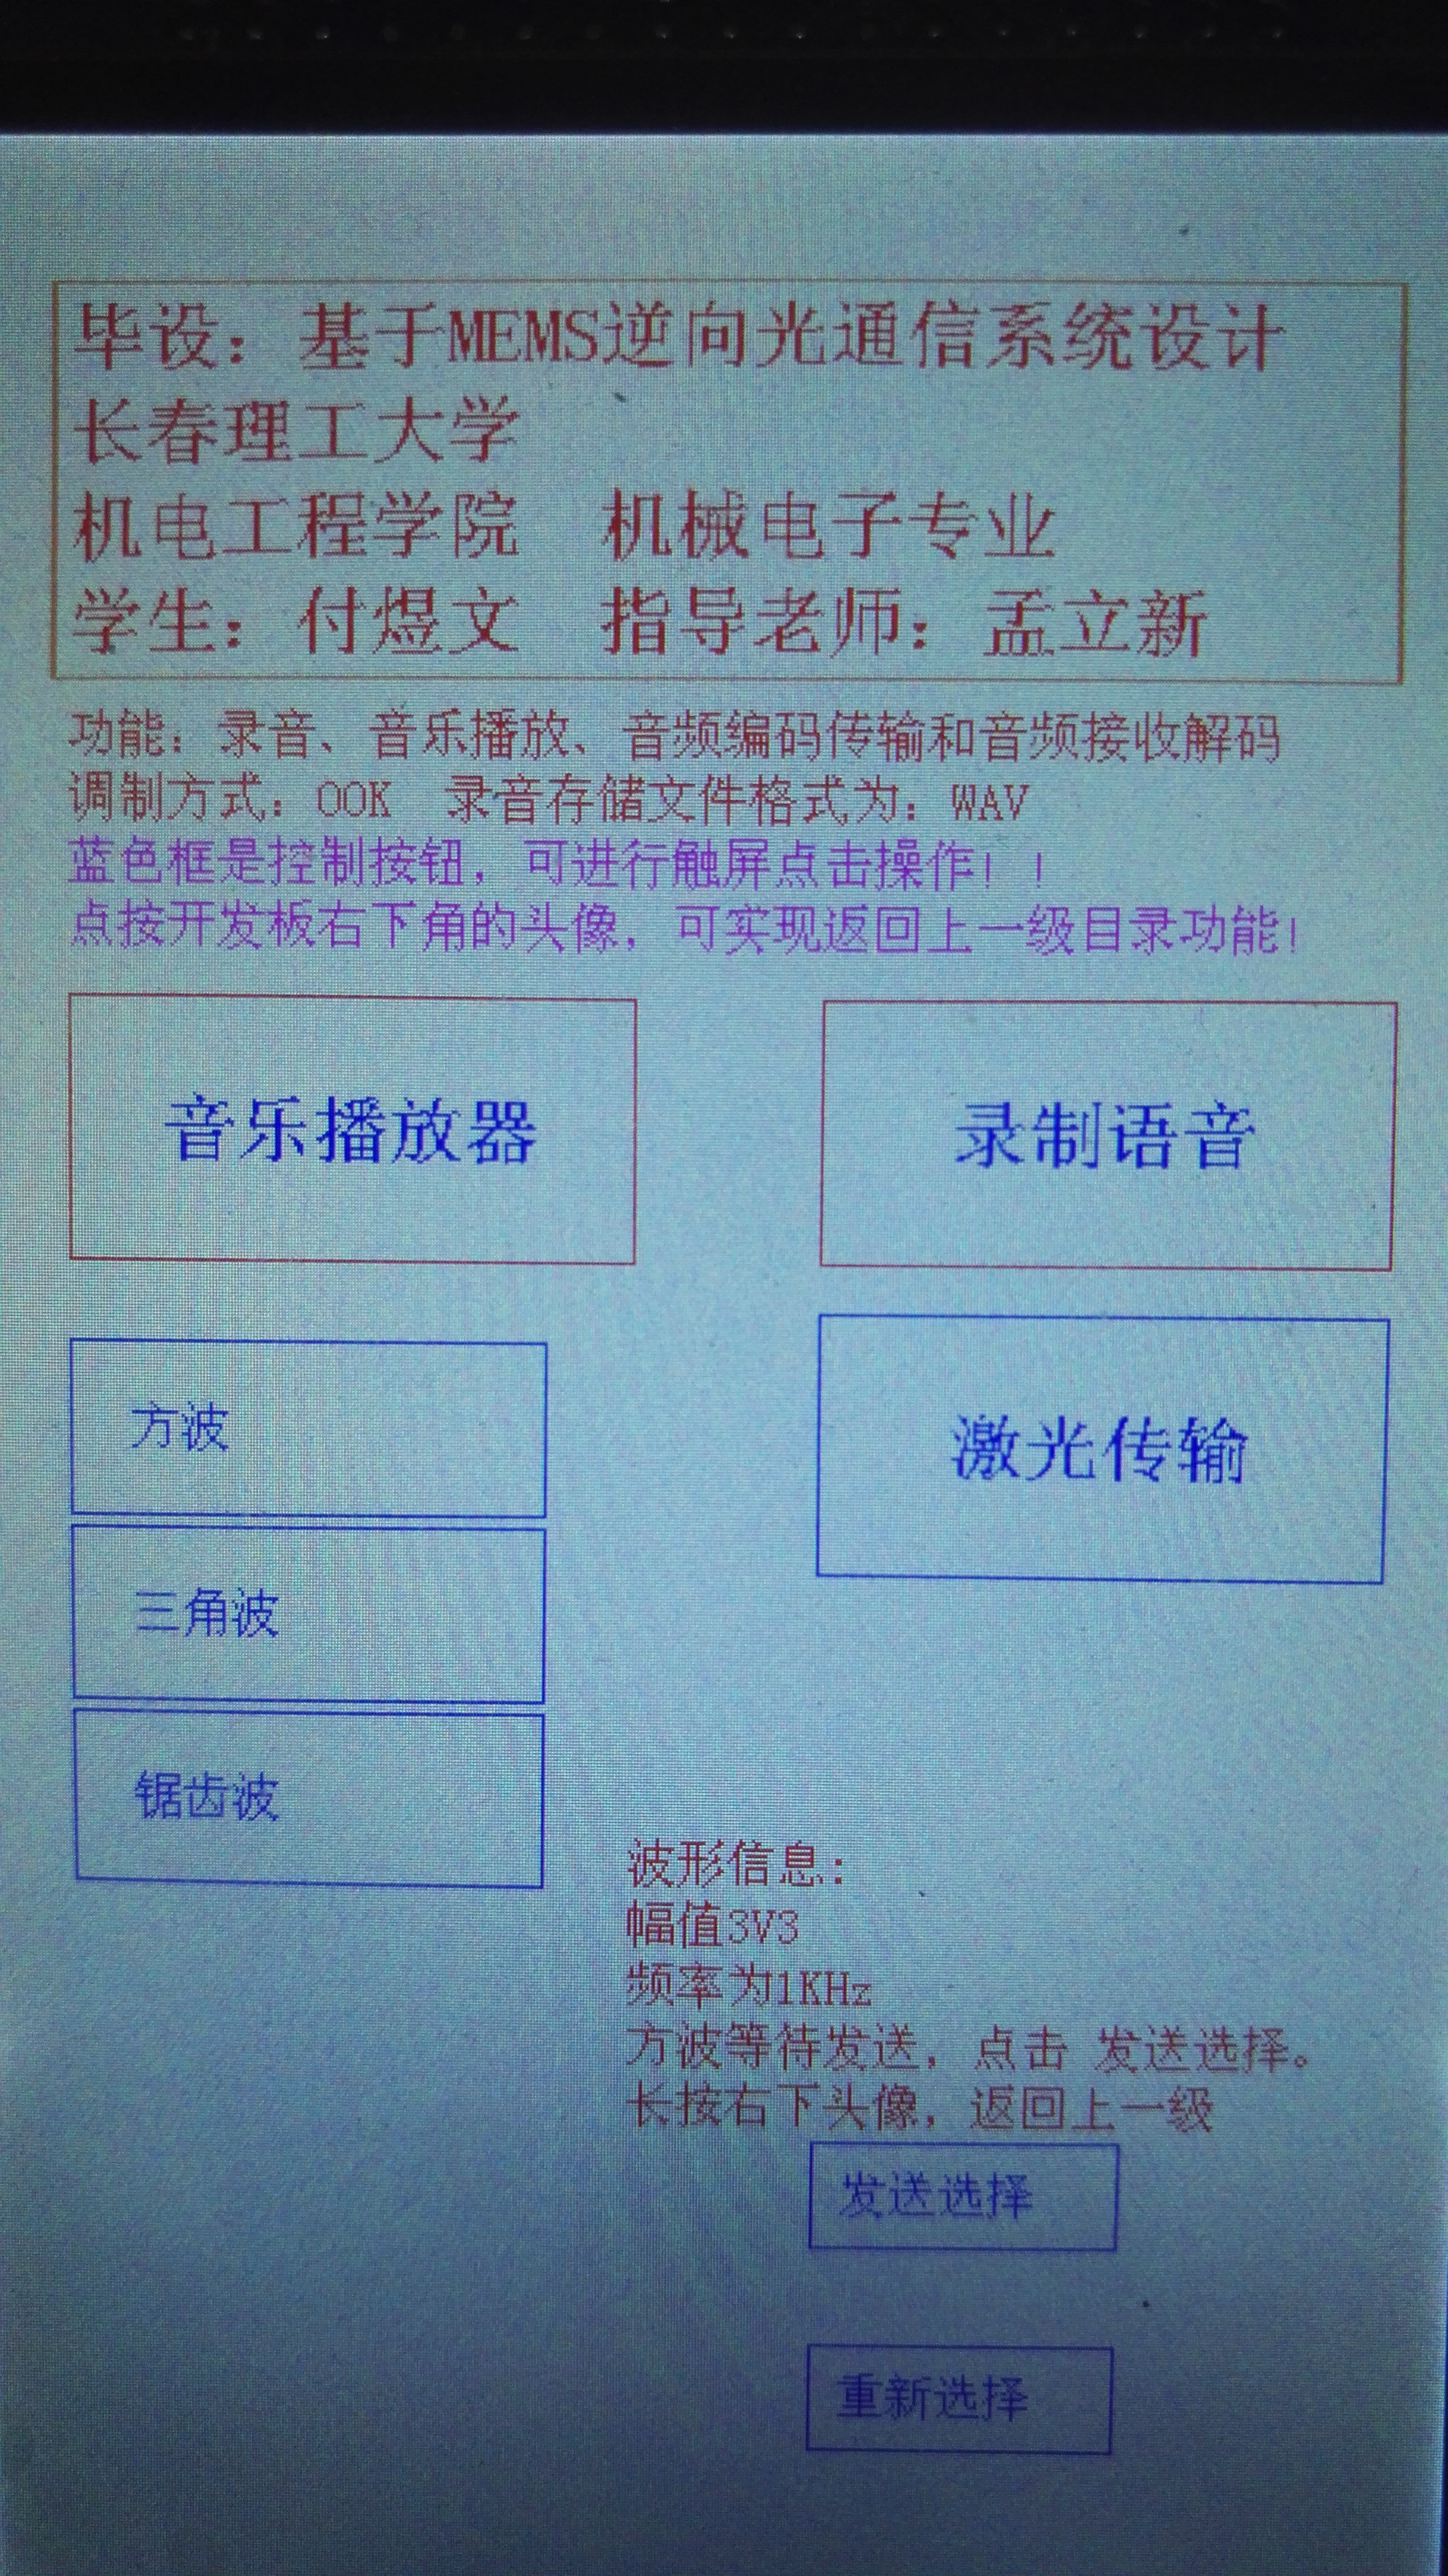
\includegraphics[width=\textwidth]{./Img/GUI-2-TRANS-1.jpg}
		\caption{激光传输的二级菜单:测试模式}
		\label{GUI-2-TRANS-1.jpg}
	\end{subfigure}%
	\caption{GUI界面的二级菜单:激光传输}
	%\bicaption{GUI界面的二级菜单:激光传输。(a) 激光传输主菜单,(b)激光传输的二级菜单:测试模式。}{}
\end{figure}

图~\ref{GUI-2-TRANS1.jpg}中展示的是GUI界面的二级菜单:激光传输——测试模式;GUI界面的二级菜单:激光传输——发送模式;GUI界面的二级菜单:激光传输——接收模式。


图~\ref{GUI-2-TRANS-1.jpg}中展示的是GUI界面的三级菜单:激光传输——测试模式——发送波形选择。



\begin{figure}[!htbp]
	\centering
	\begin{subfigure}[c]{0.4\textwidth}
	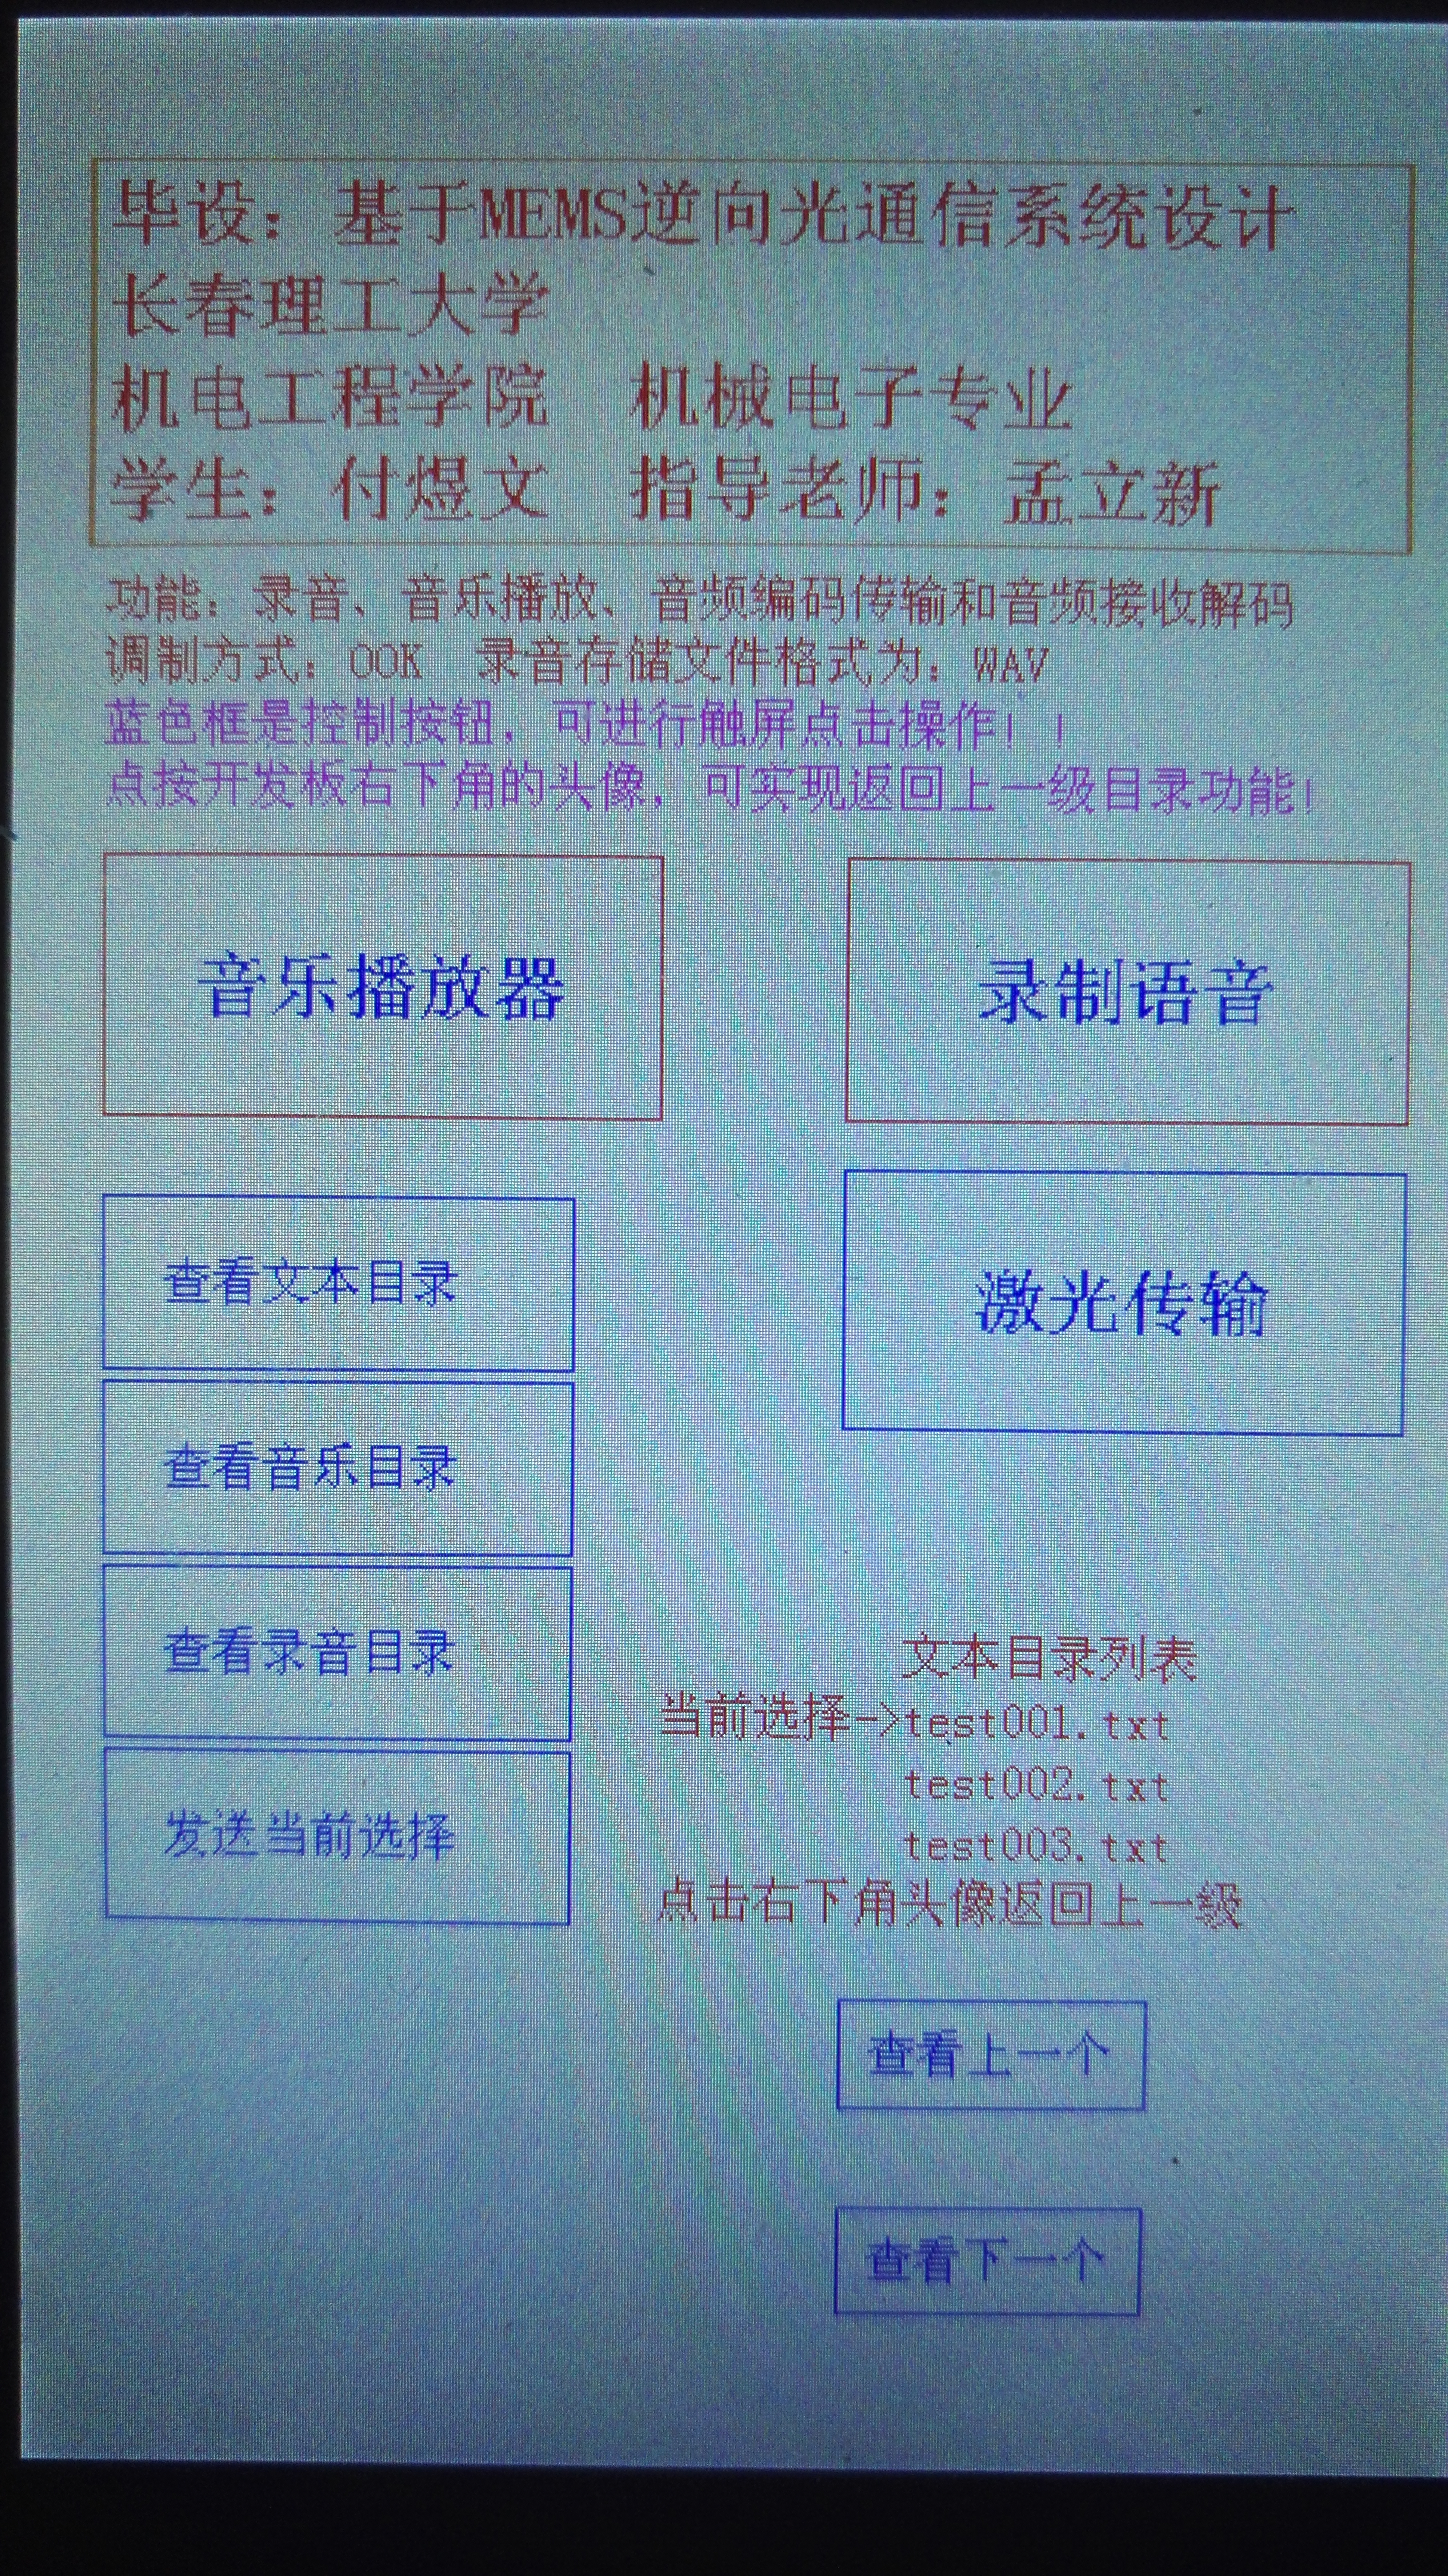
\includegraphics[width=\textwidth]{./Img/GUI-2-TRANS-2.jpg}
	\caption{目录查看}
	\label{GUI-2-TRANS-2.jpg}
	\end{subfigure}%
	~
	\begin{subfigure}[c]{0.4\textwidth}
		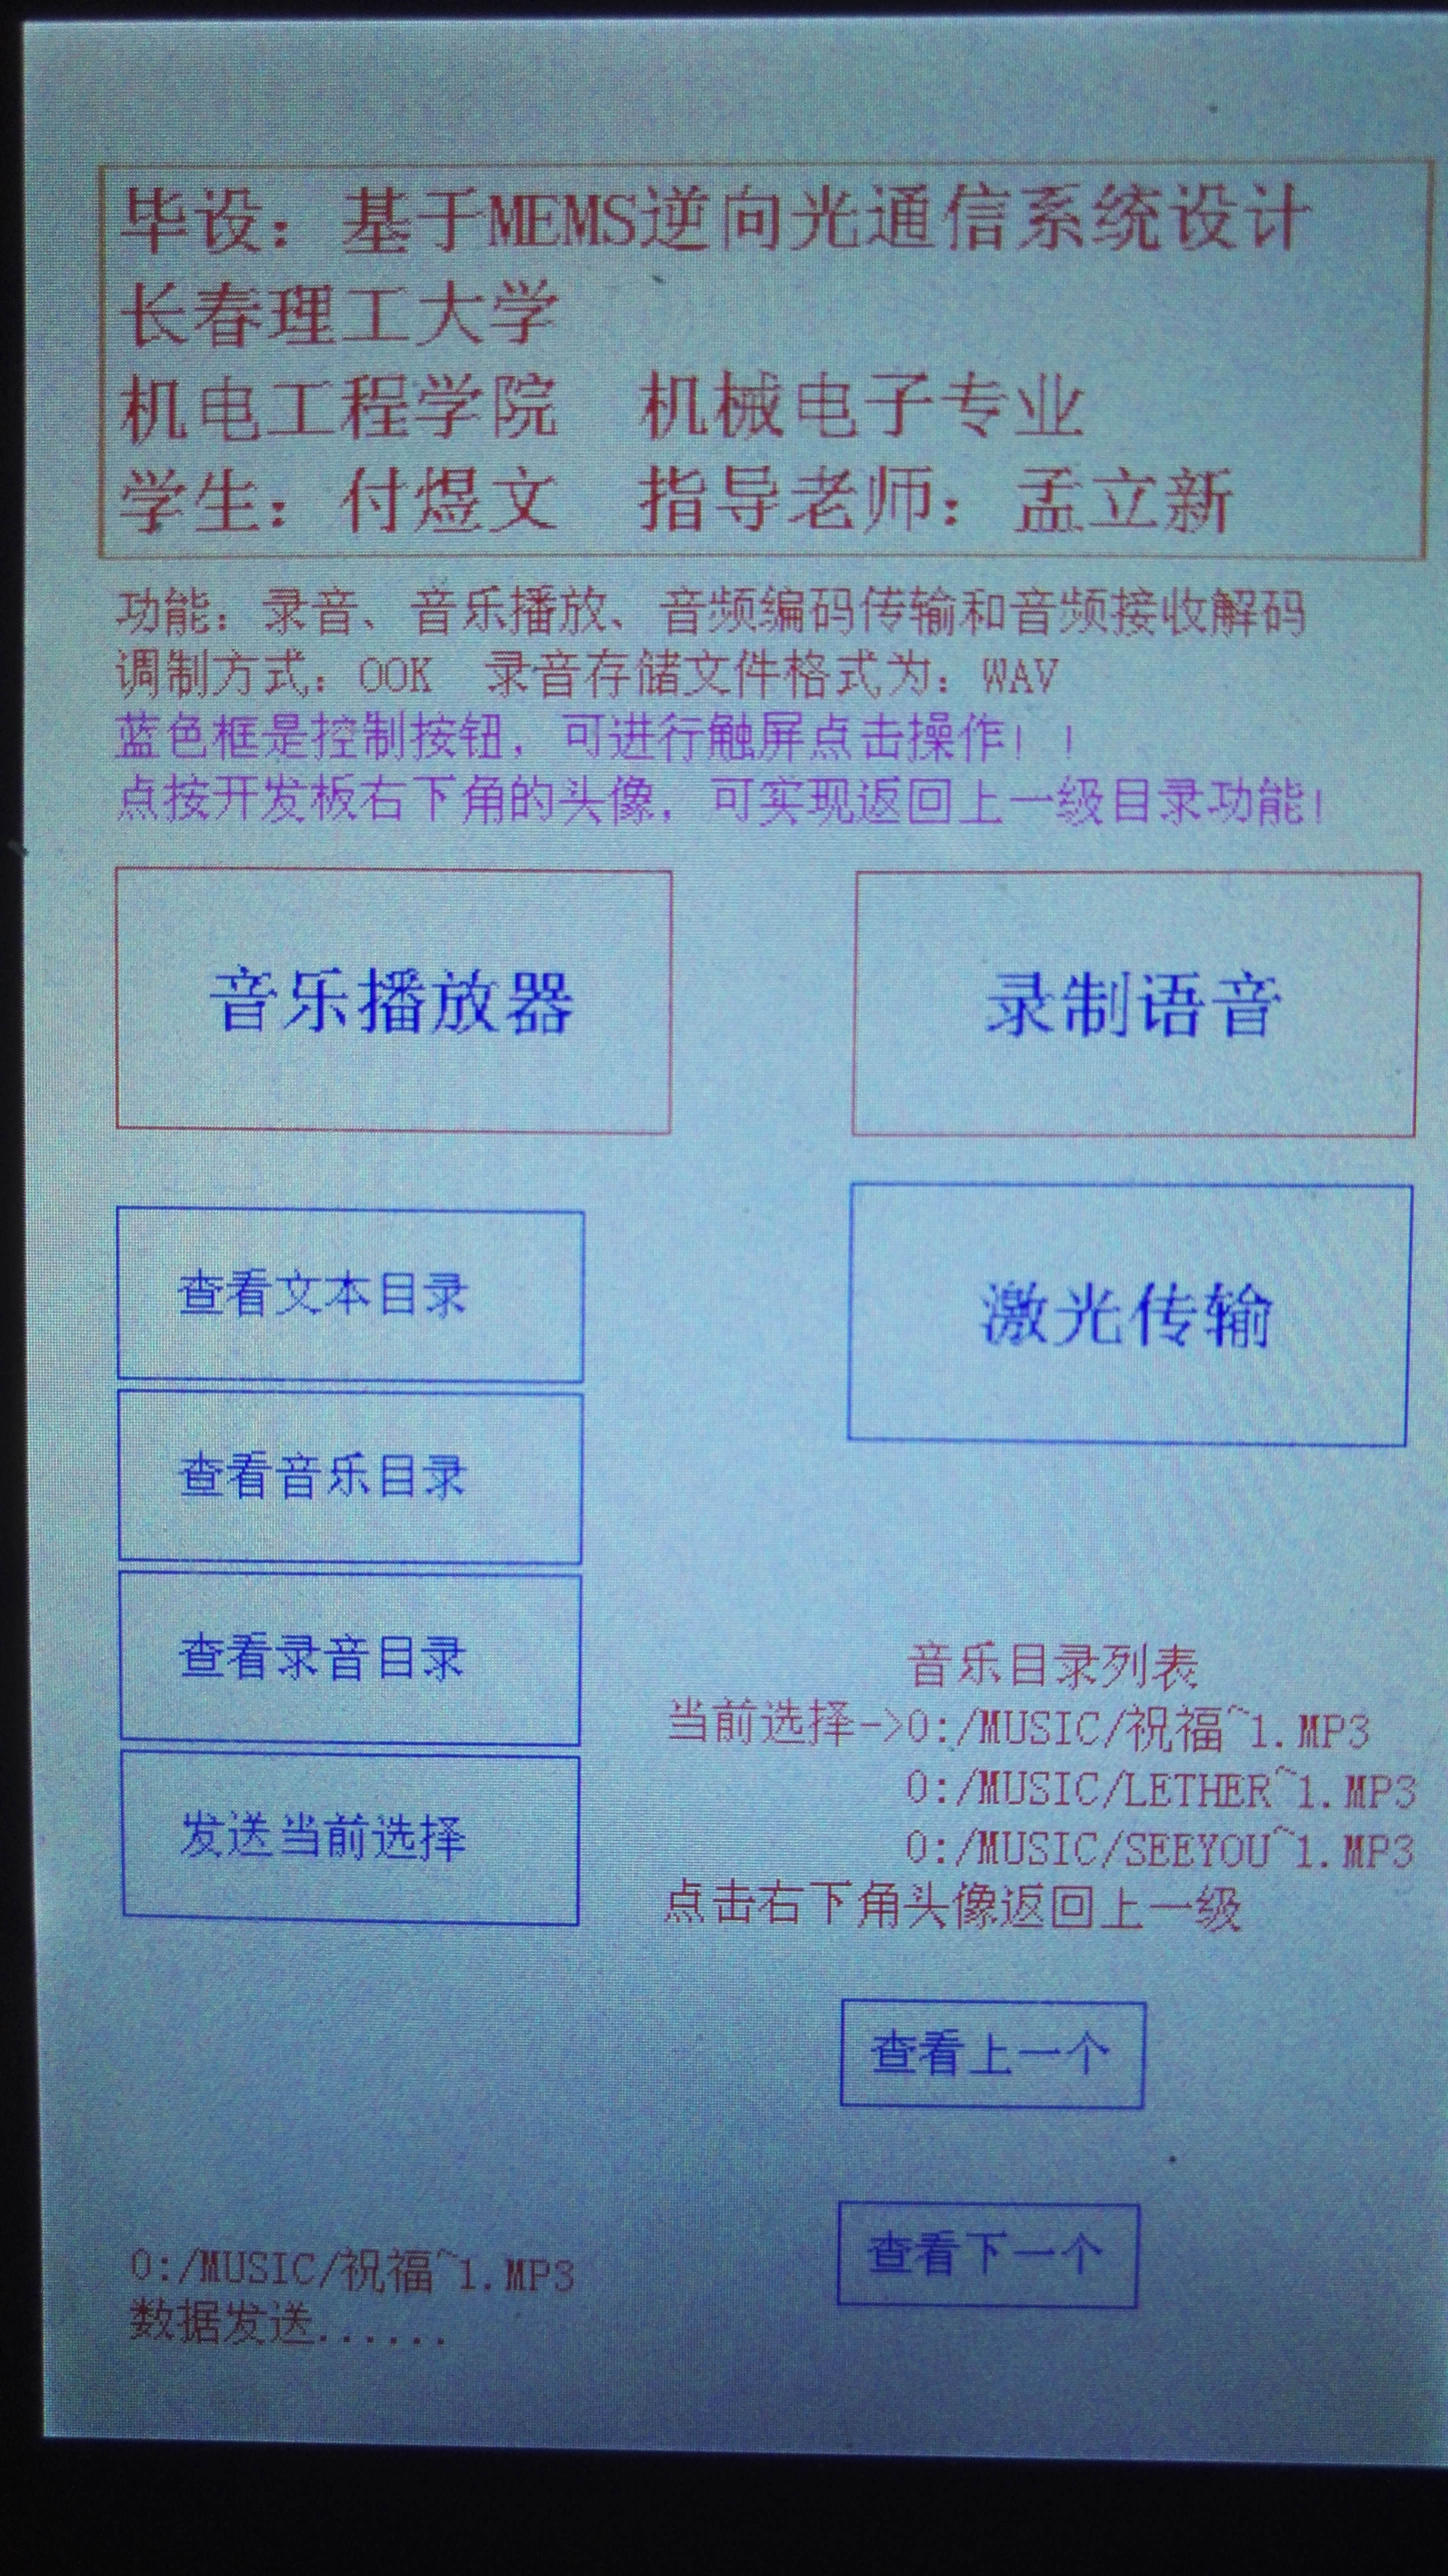
\includegraphics[width=\textwidth]{./Img/GUI-2-TRANS-2-1.jpg}
		\caption{数据正在发送}
		\label{GUI-2-TRANS-2-1.jpg}
	\end{subfigure}%
	
	%add desired spacing
	\begin{subfigure}[c]{0.4\textwidth}
		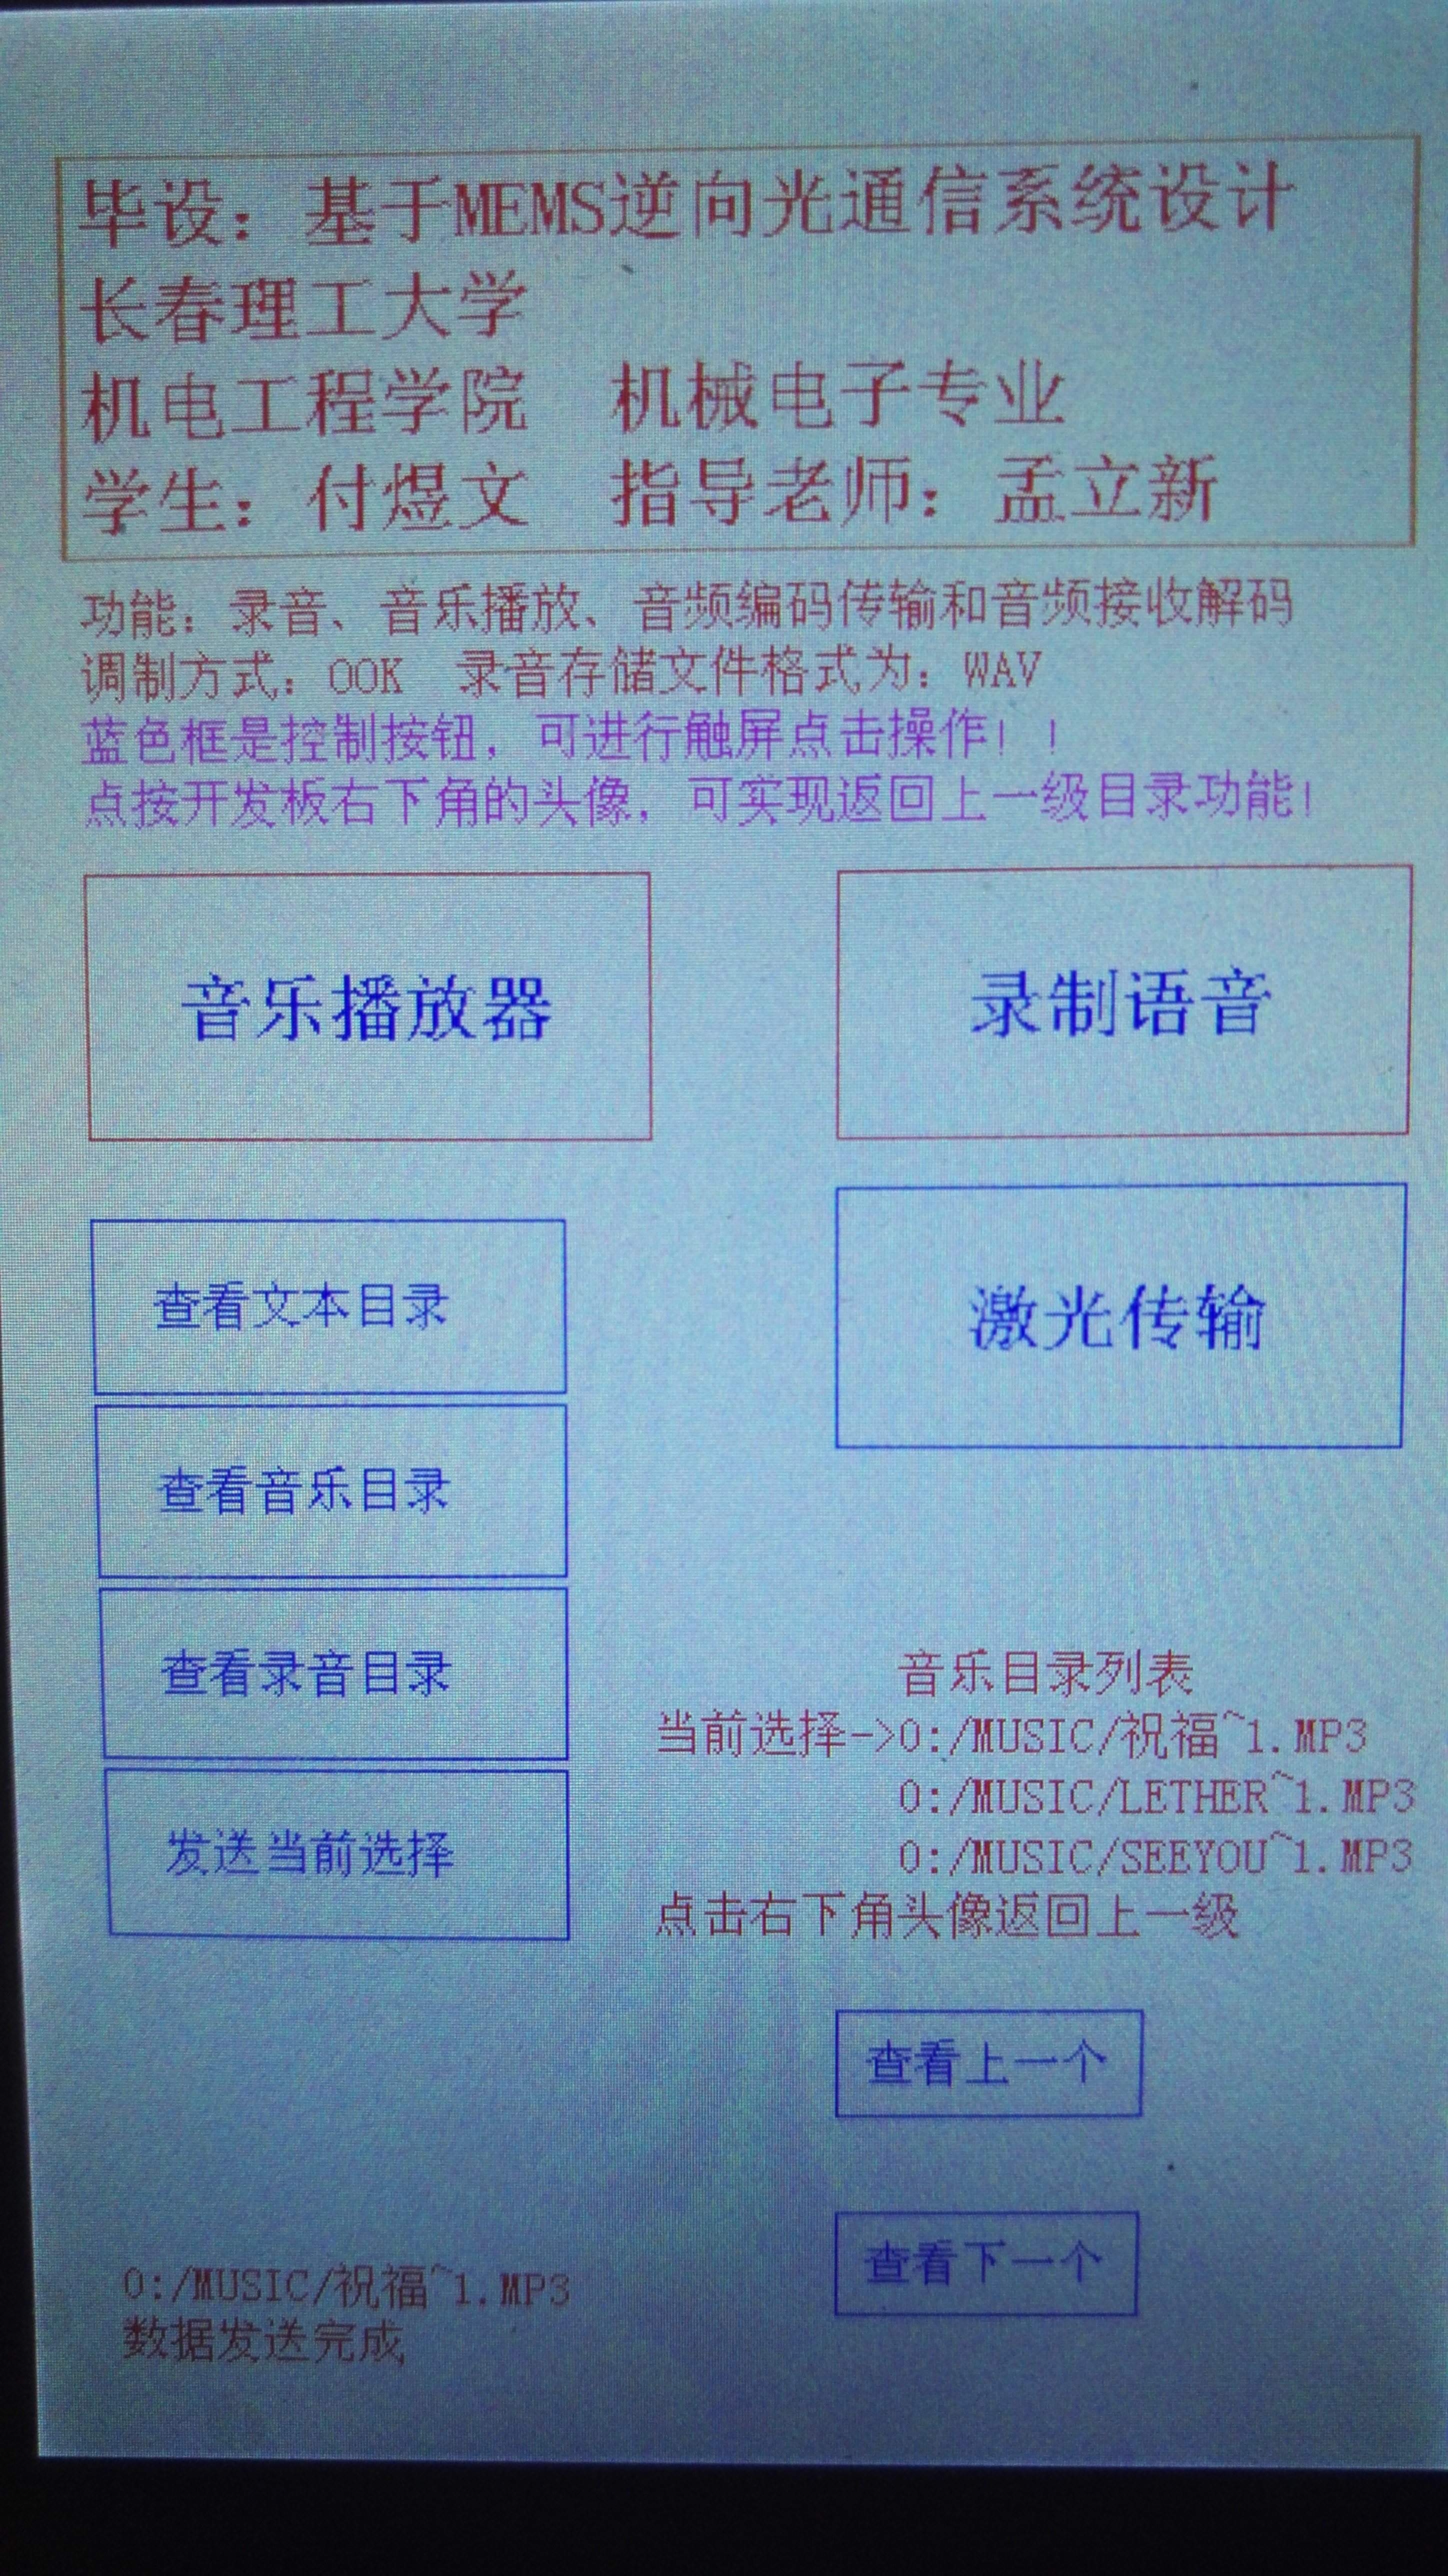
\includegraphics[width=\textwidth]{./Img/GUI-2-TRANS-2-2.jpg}
		\caption{数据发送完成}
		\label{GUI-2-TRANS-2-2.jpg}
	\end{subfigure}
	\caption{GUI界面的三级菜单:激光传输——发送模式}
	%\bicaption{GUI界面的三级菜单:激光传输——发送模式。(a)目录查看,(b)数据正在发送 ,(c)数据发送完成。}{}
\end{figure}

图~\ref{GUI-2-TRANS-2.jpg}中展示的是GUI界面的三级菜单:激光传输——发送模式,图~\ref{GUI-2-TRANS-2-1.jpg}和图~\ref{GUI-2-TRANS-2-2.jpg}中展示选择目录文件进行发送的过程。


\begin{figure}[!htbp]
	\centering
	\begin{subfigure}[c]{0.4\textwidth}
		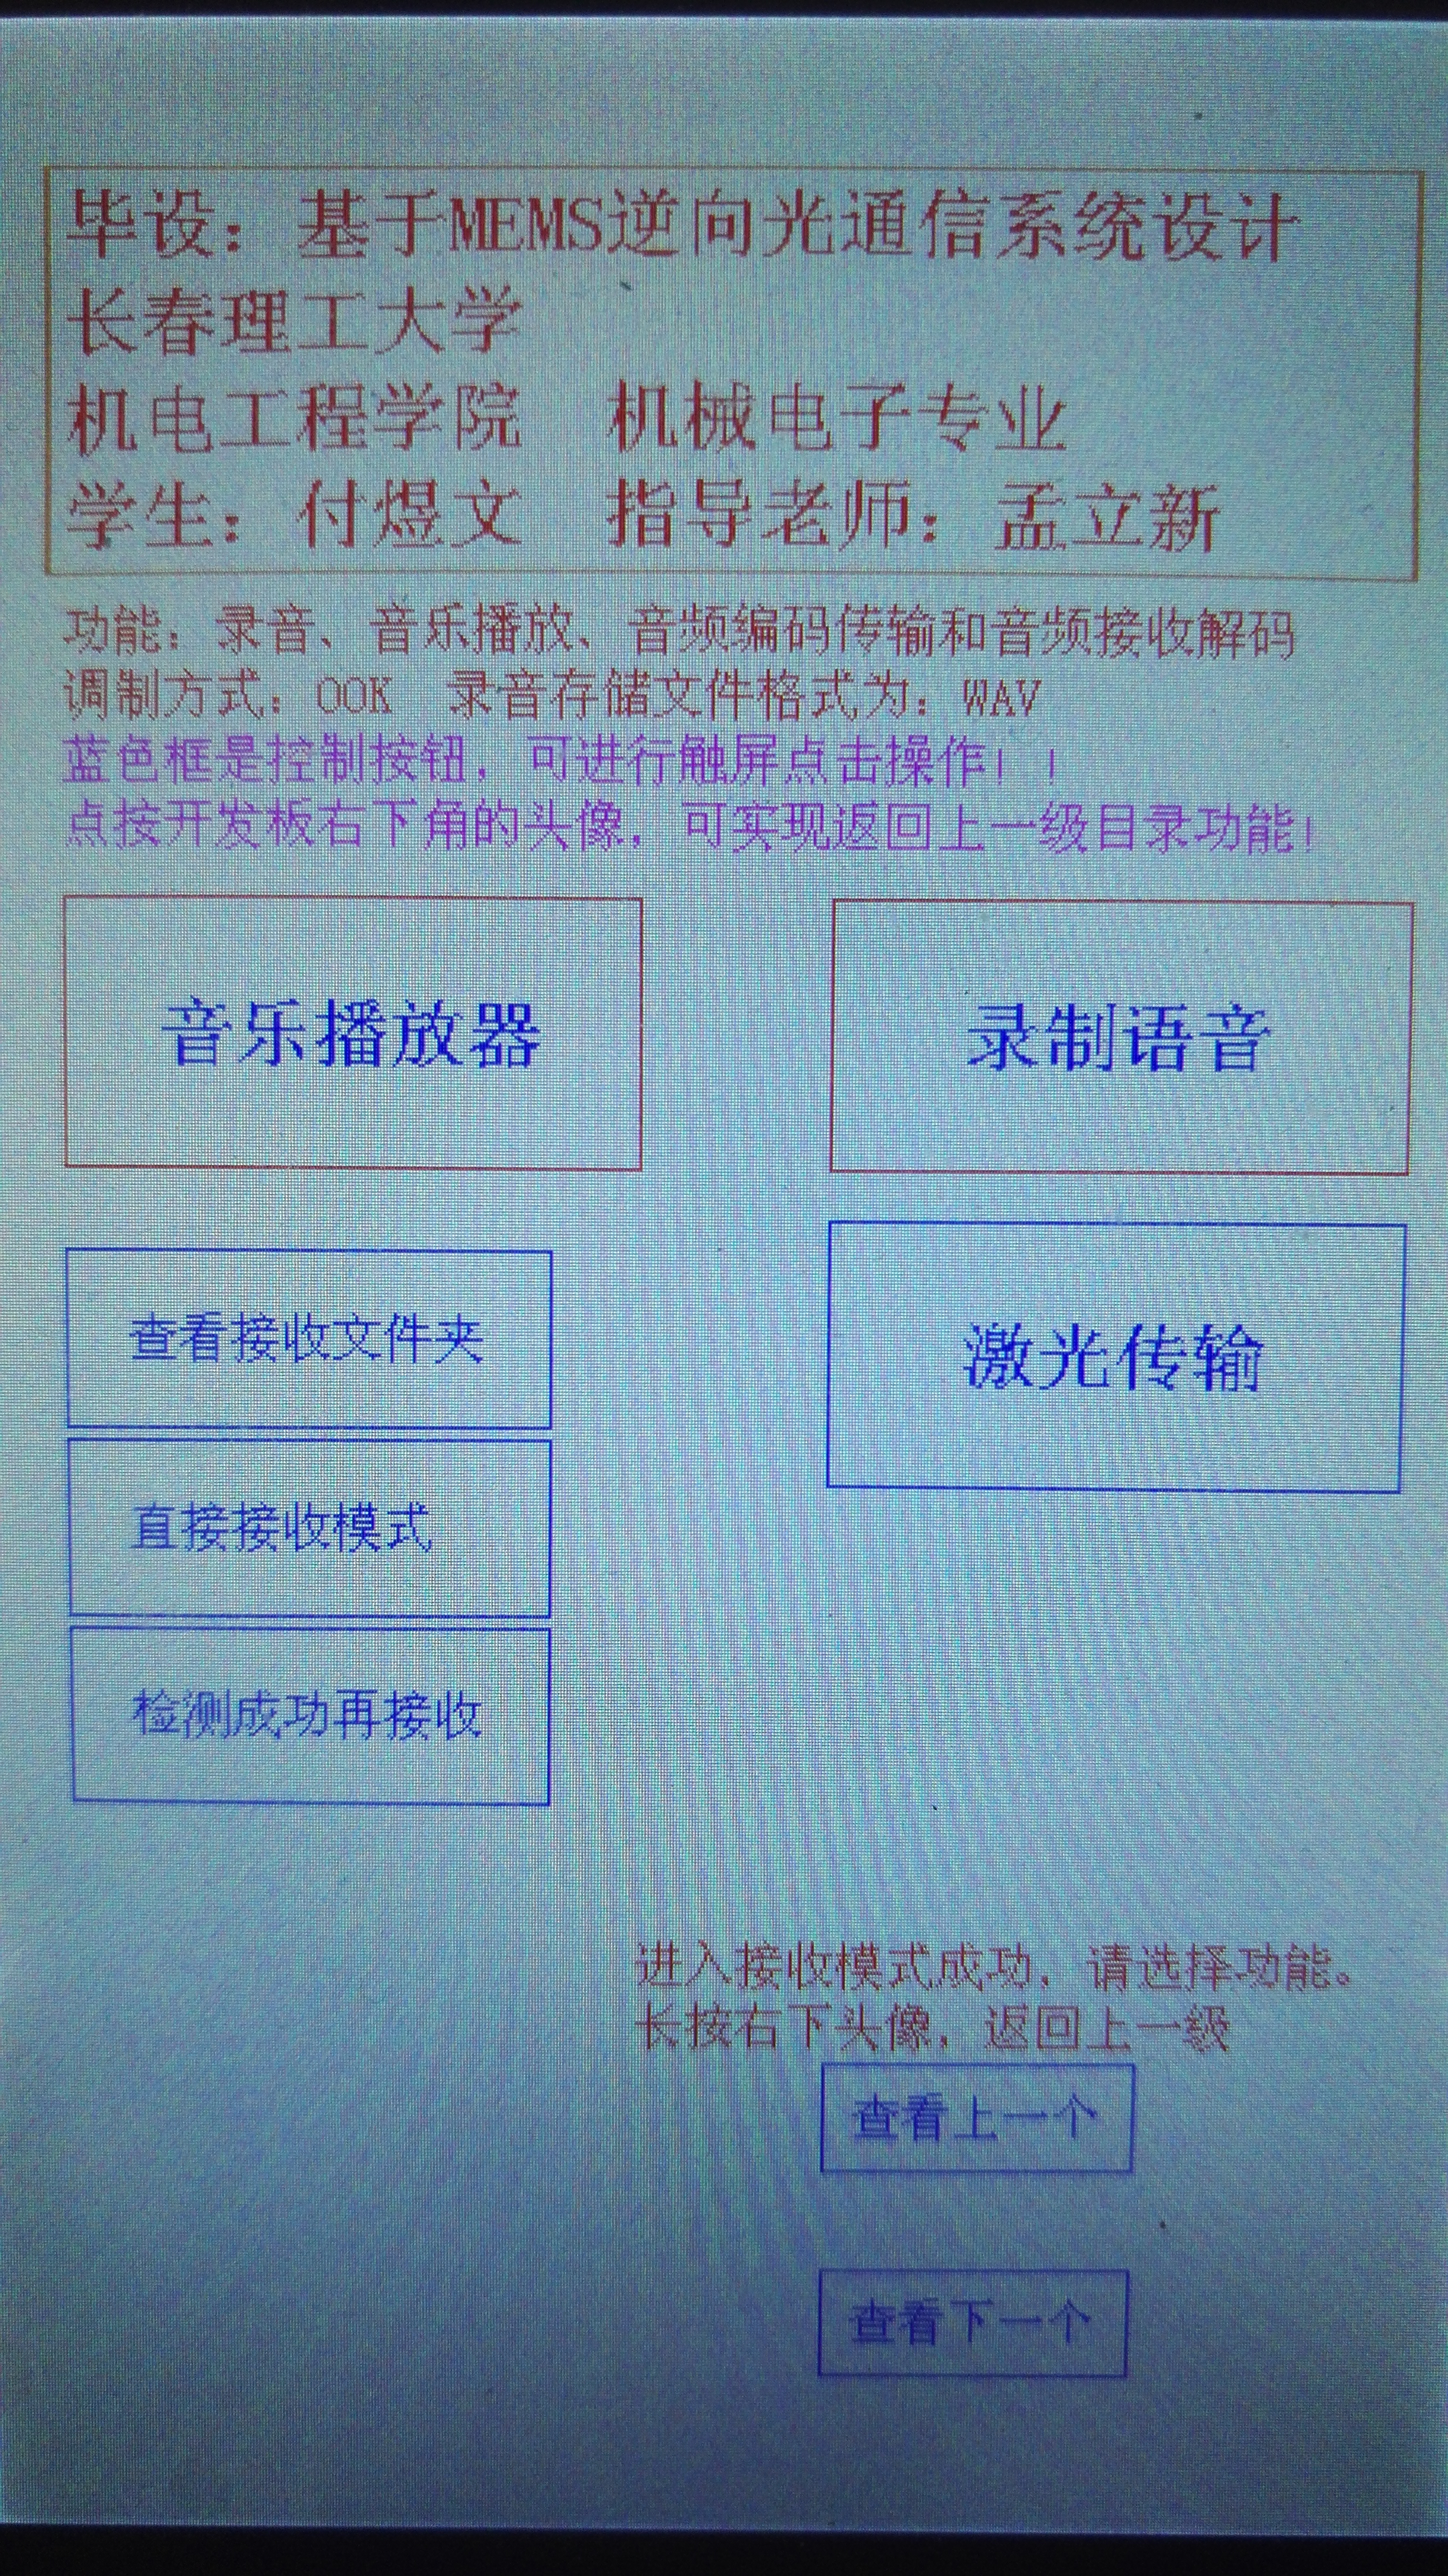
\includegraphics[width=\textwidth]{./Img/GUI-3-TRANS-3.jpg}
		\caption{接收模式的主菜单}
		\label{GUI-3-TRANS-3.jpg}
	\end{subfigure}
	~	
	\begin{subfigure}[c]{0.4\textwidth}
		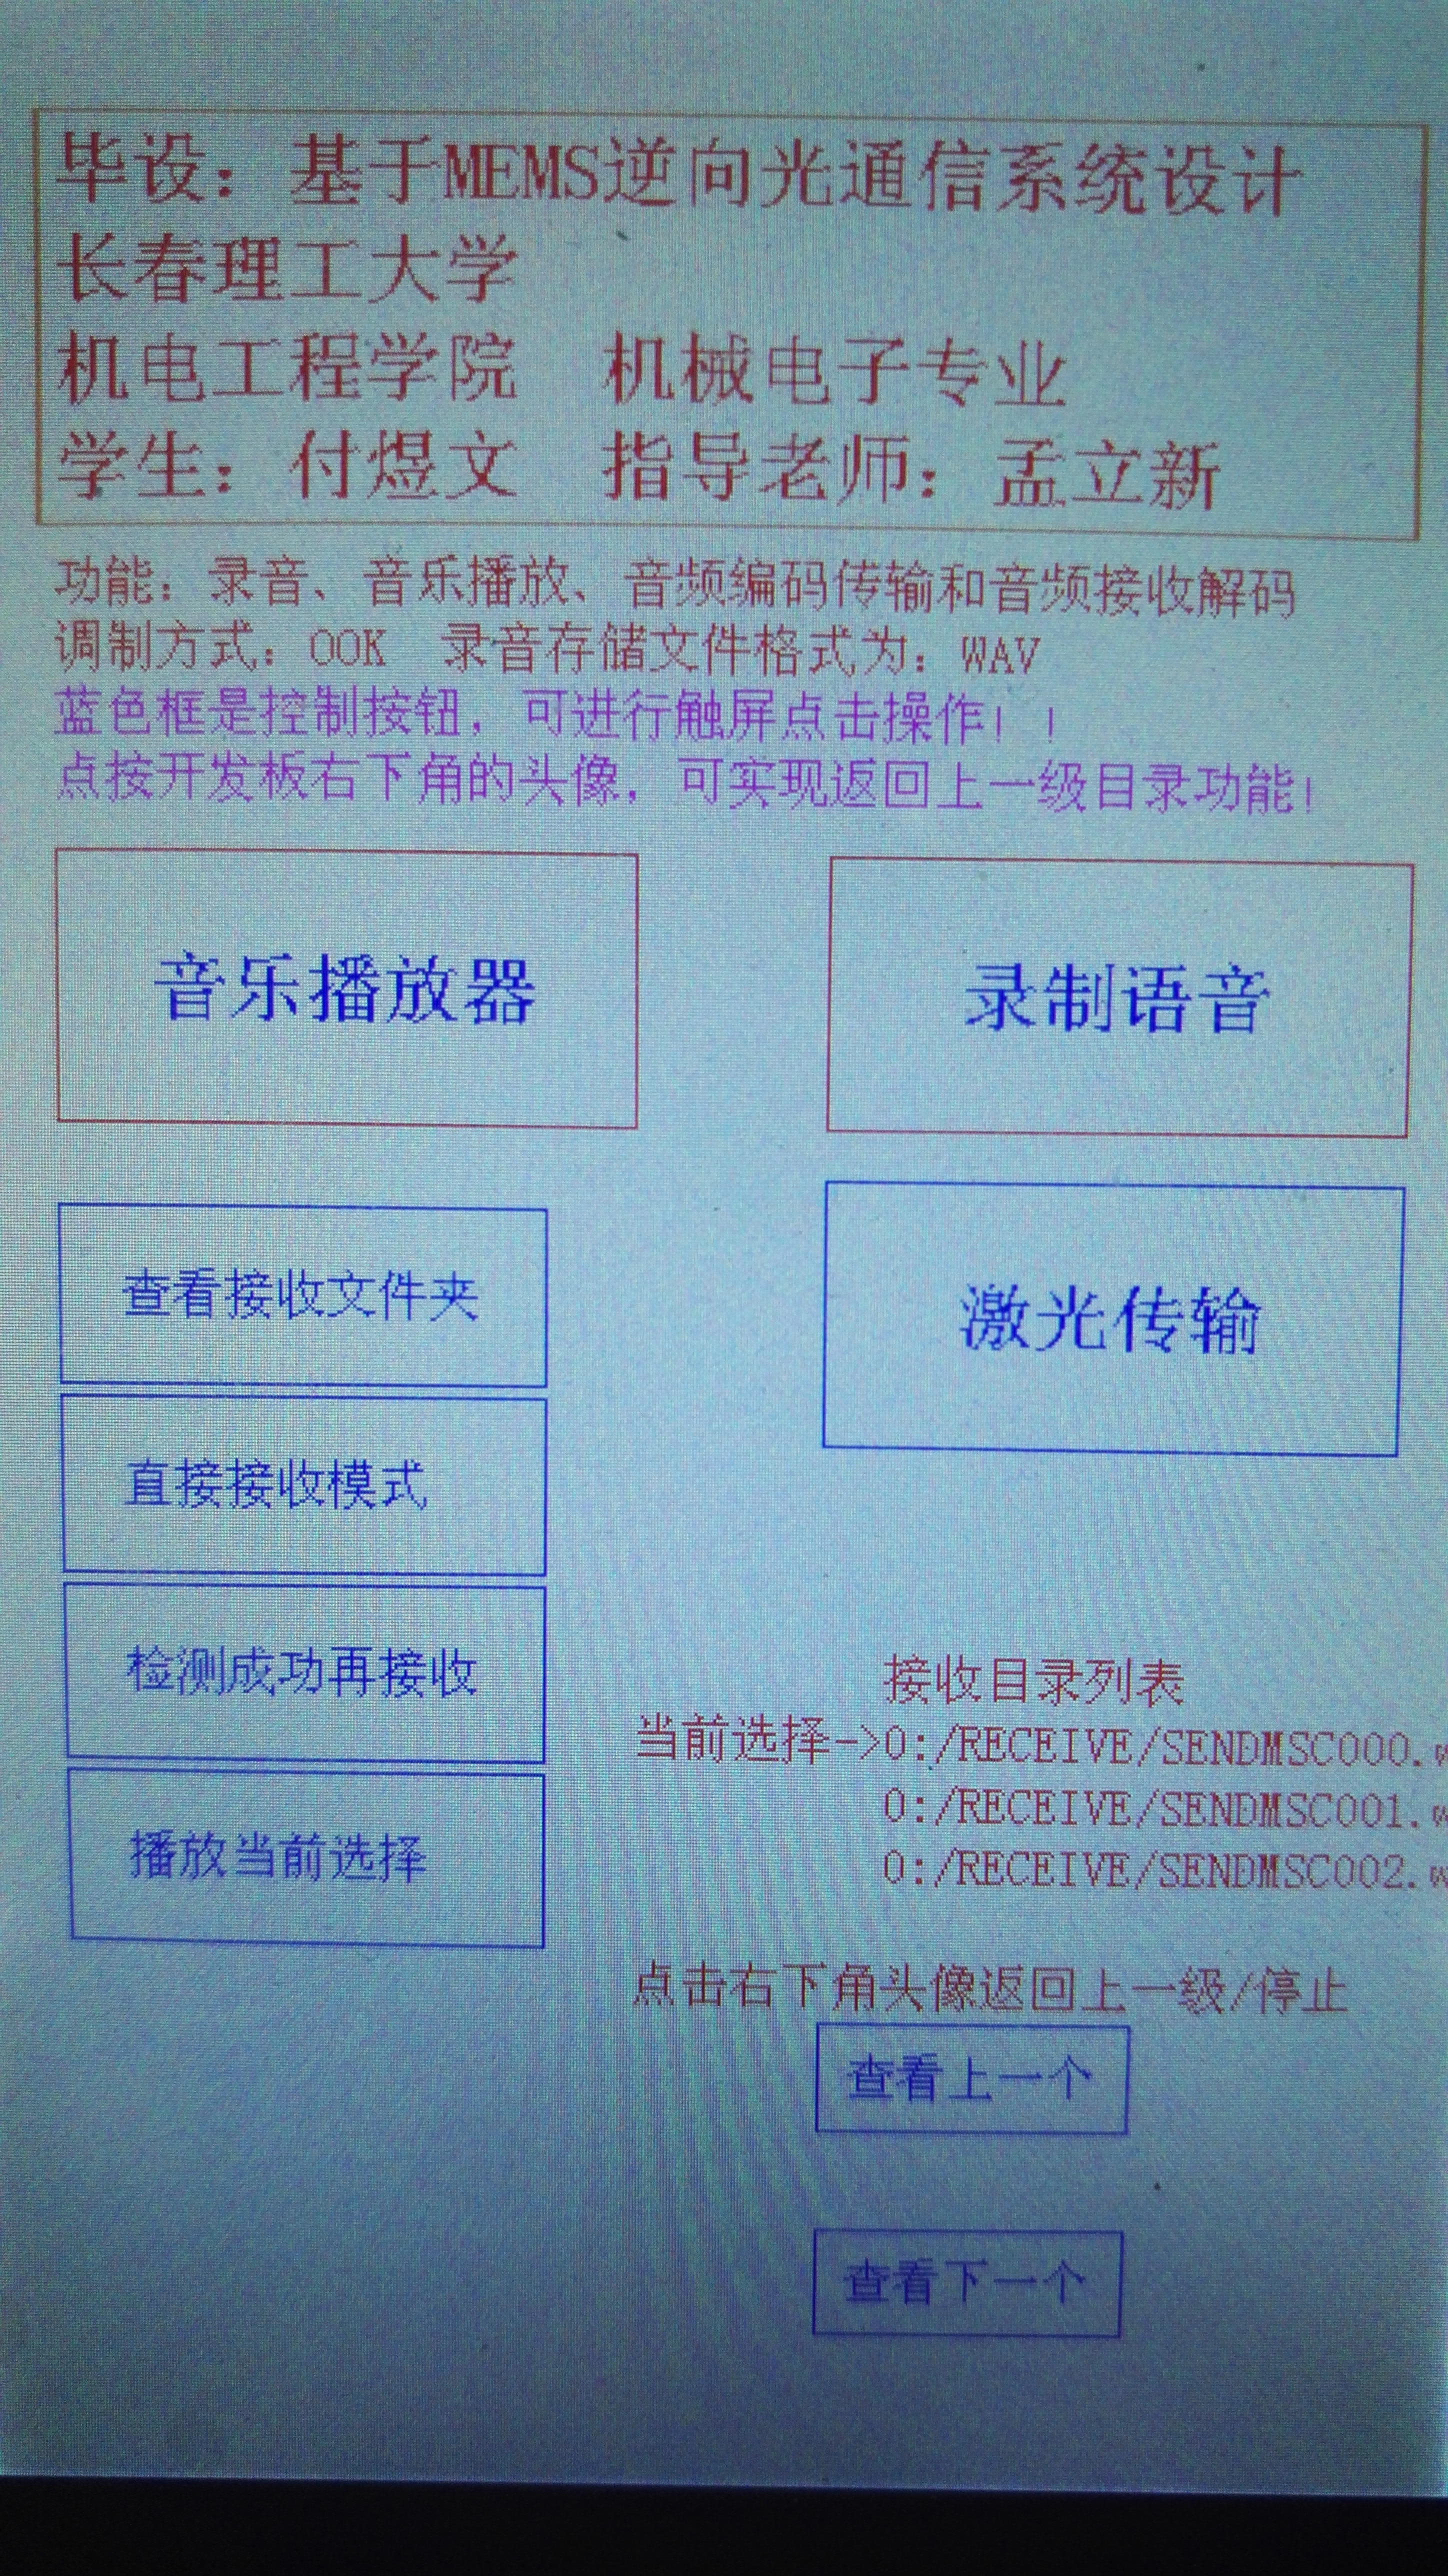
\includegraphics[width=\textwidth]{./Img/GUI-3-TRANS-3-1.jpg}
		\caption{查看接收文件的目录}
		\label{GUI-3-TRANS-3-1.jpg}
	\end{subfigure}%
	\caption{GUI界面的三级菜单:激光传输——接收模式}
%	\bicaption{GUI界面的三级菜单:激光传输——接收模式。(a) 接收模式的主菜单,(b)查看接收文件的目录}{}
\end{figure}

图~\ref{GUI-3-TRANS-3.jpg}和~\ref{GUI-3-TRANS-3-1.jpg}中展示的是GUI界面的三级菜单:激光传输——接收模式界面。
